\documentclass[output=paper,modfonts]{langscibook} 
\ChapterDOI{10.5281/zenodo.1469555}
\title{PARSEME multilingual corpus of verbal multiword expressions} 
\author{
Agata Savary$^1$,
Marie Candito$^2$,
Verginica Barbu Mititelu$^3$,
Eduard Bejček$^4$,
Fabienne Cap$^5$,
Sla\-vo\-mír Čéplö$^6$,
Silvio Ricardo Cordeiro$^7$,
Gülşen Eryiğit$^8$,
Voula Giouli$^9$,
Maarten van Gom\-pel$^{10}$,
Yaakov HaCohen-Kerner$^{11}$,
Jolanta Kovalevskaitė$^{12}$,
Simon Krek$^{13}$,
Chaya Lie\-bes\-kind$^{11}$,
Johanna Monti$^{14}$,
Carla Parra Escartín$^{15}$,
Lonneke van der Plas$^6$, 
Behrang QasemiZadeh$^{16}$,
Carlos Ramisch$^7$,
Fe\-de\-ri\-co Sangati$^{17}$,
Ivelina Stoyanova$^{18}$ \&
Veronika Vincze$^{19}$
\affiliation{%
$^1$Université de Tours (France), 
$^2$Université Paris Diderot (France), 
$^3$Romanian Acad\-e\-my Research Institute for Artificial Intelligence (Romania), 
$^4$Charles University (Czech Republic), 
$^5$Uppsala University (Sweden), 
$^6$University of Malta (Malta), 
$^7$Aix Marseille University (France), 
$^8$Istanbul Technical Uni\-ver\-si\-ty (Tur\-key), 
$^9$Ath\-ena Research Center in Athens (Greece), 
$^{10}$Radboud University in Nijmegen (Netherlands),
$^{11}$Je\-ru\-sa\-lem College of Technology (Israel),
$^{12}$Vy\-tau\-tas Ma\-gnus Uni\-ver\-si\-ty in Kau\-nas (Lithuania), 
$^{13}$Jožef Stefan Institute in Ljubljana (Slovenia), 
$^{14}$``L'Orientale'' University of Naples (Italy), 
$^{15}$ADAPT Centre, Dublin City University (Ireland), 
$^{16}$University of Düsseldorf (Germany), 
$^{17}$independent re\-sear\-cher (Italy), 
$^{18}$Bulgarian Academy of Sciences in Sofia (Bulgaria), 
$^{19}$Univer\-sity of Szeged (Hungary)
}
}


%Agata Savary, Kübra Adali, Eduard Bejček, Marie Candito, Fabienne Cap, Silvio Ricardo Cordeiro, Gülşen Eryiğit, Luke Galea, Voula Giouli, Maarten van Gompel, Yaakov HaCohen-Kerner, Jolanta Kovalevskaite, Simon Krek, Chaya Liebeskind, Verginica Mititelu, Johanna Monti, Carla Parra, Lonneke van der Plas, Behrang QuasemiZadeh, Carlos Ramisch, Federico Sangati, Ivelina Stoyanova and Veronika Vincze
 
\abstract{
Multiword expressions (MWEs) 
%\fc{changed this from multiword to  multiword as it appeared to me that the latter one is used more frequently throughout the text.} \capa{We should probably agree on a spelling and be consistent with it throughout the whole chapter.} 
are known as a ``pain in the neck'' due to their idiosyncratic behaviour. While some categories of MWEs have been largely studied, 
%a large number of CR
%many studies, 
verbal MWEs (VMWEs) such as \ile{to take a walk},  \ile{to break one's heart} or \ile{to turn off} have been relatively rarely modelled. 
 %This is notably due to their syntactic variability, which hinders treating them as ``words with spaces''. 
 We describe an initiative meant to bring about substantial progress in understanding, modelling and 
% automatically CR
processing VMWEs. In this joint effort carried out within a European research network we elaborated a universal terminology and annotation methodology for VMWEs. 
Its main outcomes, available under open licenses, are %universal
unified annotation guidelines, and a corpus\is{PARSEME!corpus}\is{multiword expression!annotated corpus} of over 5.4 million words and 62 thousand annotated VMWEs in 18 languages.
%which underlies a shared task on automatic identification of VMWEs. 
}


\renewcommand{\lsCollectionPaperCitationText}{Agata Savary et al. 2018. PARSEME multilingual corpus of verbal multiword expressions. 
In Stella Markantonatou, Carlos Ramisch, Agata Savary \& Veronika Vincze (eds.), 
Multiword expressions at length and in depth: Extended papers from the MWE 2017 workshop, 1–23. 
Berlin: Language Science Press. {\color{lsDOIGray} DOI: \href{http://dx.doi.org/zenodo.1469555}{10.5281/zenodo.1469555}}
}
\begin{document}
\maketitle
\label{SAVARY-CHAPTER}
\lehead{Savary et al.}%Needed to make the authors' headline shorter. Always place just after \begin{document}


%\lehead{Savary et al.}



%"H

%%%%%%%%%%%%%%%%%%%%%%%%%%%%%%%%%%%%%%%%%%%%%%%%%%%%%%%%%%%%%%%%%%%%%%%%%%%%%%%%%%%%%%%%%%%%%%%%%%%%%%%%%%%%%%%%%%%%%%%%%%%%%%%%%%%%%%%%%%%%%%%%%%%%%%%%%%%%%%%%%%%%%%%%%%%%%%%%%%%%%%%%%%%%%%%%%%%%%%%%%%%%
%%%%%%%%%%%%%%%%%%%%%%%%%%%%%%%%%%%%%%%%%%%%%%%%%%%%%%%%%%%%%%%%%%%%%%%%%%%%%%%%%%%%%%%%%%%%%%%%%%%%%%%%%%%%%%%%%%%%%%%%%%%%%%%%%%%%%%%%%%%%%%%%%%%%%%%%%%%%%%%%%%%%%%%%%%%%%%%%%%%%%%%%%%%%%%%%%%%%%%%%%%%%
\section{Introduction}
\label{sec:sav:intro}
%\input{chapters/15.intro}
%\as{Formatting guidelines:
%there should
%not be any vertical lines in tables, and as few horizontal lines as
%possible. Grouping can better be achieved with white space, e.g.
%%\begin{verbatim}
%\begin{tabular}{lll @{\qquad} lll @{\qquad} lll}
%a & a & a  &  b & b & b  &  c & c & c\\
%\end{tabular}
%This gives you three groups of three columns each.
%a a a     b b b     c c c
%%\end{verbatim}
%}
%\eb{fixed in all tables}

%\as{Avoid overlapping with the introduction to the ST organization paper. }
One of the basic ideas underlying linguistic modelling is compositionality\is{compositionality} \citep{Baggioetal12}, seen as a property of language items \citep{Janssen01,Parteeetal90} or of linguistic analyses \citep{Kracht07}. 
Counterexamples which challenge the compositionality principles \citep{PaginWesterstahl10b} include multiword expressions (MWEs) \citep{Sag2002a,Kim:2008}%,calzolari-et-al:2002}
, and notably 
%. It emerged as early as with Frege \citep{Janssen01} and has been a central topic of debate since then. Some authors \citep{Parteeetal90} assume that a compound expression is compositional if its meaning is a function of the meanings of its parts and of the syntactic rule by which they are combined. Others \citep{Kracht07} state that compositionality is a property of linguistic analyses rather than of the language itself. While there are many reasons for promoting compositionality in linguistic analyses \citep{Baggioetal12}, certain constructions are counterexamples which challenge the compositionality principles \citep{PaginWesterstahl10b}. These include multiword expressions (MWEs), which display lexical, syntactic, semantic, pragmatic and/or statistical idiosyncrasy \citep{Sag01multiwordexpressions,Kim:2008,calzolari-et-al:2002}.
verbal MWEs (VMWEs)\is{verbal multiword expression}, such as (\ref{sl:skrivati-glavo-v-pesek}--\ref{ro:se-face}).\footnote{See the preface for the description of the conventions used to present multilingual examples.}
%\footnote{The index of abbreviations in p.~\pageref{sec:abbreviations} gives the meaning of all language codes and of the grammatical codes used in glosses. Henceforth, multilingual itemized VMWE examples will contain: (i) a sample use of the VMWE, followed by the language code; (ii) a transcription, if the language is written with a non-Latin alphabet; (iii) a gloss, (iv) a literal translation, followed by an idiomatic translation in single quotes. For right-to-left languages (Farsi and Hebrew), item (i) will be spelled right-to-left, item (iv) left-to-right and items (ii--iii) left-to-right within components, and right-to-left from one component to another. 
%Lexicalized components of the VMWE, i.e. those which are always realized by the same lexeme (Sec.~\ref{sec:def-scope}) will be highlighted in bold face. In-line examples, used for brevity, will be preceded by the language code and will contain items (i) and (iv) only, and the idiomatic translation (if any) will be introduced by a double arrow `$\Rightarrow$'. In each usage example the head verb will be either in a finite form or in the infinitive (only when the subject is not lexicalized). We put forward these conventions as a future notation standard for multilingual examples of MWEs.}
%\eb{In the footnote, I would say "abbreviations on p.~\pageref{sec:abbreviations}" (i.e. preposition and only one 'p' since it's on one page).}  
%\as{Please, provide a transcription for Greek and a finite verb example for Romanian.}
%(SL) \exlitidio{\lex{skrivati glavo v pesek}}{to hide  one's head in the sand}{to pretend not to see a problem}, (DE) \exlitidio{er \lex{legt} die Prüfung \lex{ab}}{he lays the exam off}{he takes the exam}, (EL) \exidio{\lex{παίρνω} μία \lex{απόφαση}}{to make a decision}, or (RO) \exlitidio{a \lex{se face}}{to self make}{to become}. 

%\begin{exe}
%\ex \label{sl:skrivati-glavo-v-pesek}
%\gll Ida \lex{skriva} \lex{glavo} \lex{v} \lex{pesek} (SL)\\
%Ida hide.\textsc{3.sg} head in sand \\
%\trans Ida hides her head in the sand `Ida pretends not to see a problem’

\ea \label{sl:skrivati-glavo-v-pesek}
\settowidth \jamwidth{(SL)} 
\gll Ida \lex{skriva} \lex{glavo} \lex{v} \lex{pesek}. \\
Ida hide.\textsc{3.sg} head in sand \\ \jambox{(SL)}
% Eva thrusts head in sand \\
\glt Ida hides her head in the sand. \idio{Ida pretends not to see a problem.}
\z

\ea \label{de:pruefung-ablegen}
\settowidth \jamwidth{(DE)} 
\gll Er \lex{legt} die Prüfung \lex{ab}. \\
he lay.\textsc{3.sg} the exam \textsc{part} \\ \jambox{(DE)}
% Eva thrusts head in sand \\
\glt He lays the exam \textsc{part}. \idio{He takes the exam.}
\z

\ea \label{el:take-decision}
\settowidth \jamwidth{(EL)} 
\glll Η Ζωή \lex{παίρνει} μία \lex{απόφαση}.\\
i zoi perni mia apofasi \\
the Zoe take.\textsc{3.sg} a decision \\ \jambox{(EL)}
\glt Zoe takes a decision. \idio{Zoe makes a decision.}
\z

\ea \label{ro:se-face}
\settowidth \jamwidth{(RO)} 
\gll Alina \lex{se} \lex{face} doctor.\\
Alina \textsc{refl.3.sg} make.\textsc{3.sg} doctor \\ \jambox{(RO)}
\glt Alina \textsc{refl} makes doctor. \idio{Alina becomes a doctor.}
\z

%\begin{minipage}{\linewidth}
%\ea\label{fr:porterculotte} 
%\langinfo{French}{Indo-European}{personal knowledge}\\
%porter la culotte `\textbf{wear the pants}'\\
%\gll Mme et M. Armand y r\'egnent paternellement, {bien que} \textbf{la culotte} y soit \textbf{port\'ee} par
%madame \ldots\\
%Mrs and Mr Armand there rule paternally {though} the pants there is worn by madam\\
%\glt 
%Mrs and Mr Armand there rule paternally although the pants are %worn by madam.\\
%`\ldots though she is dominant'\label{fr-culotte}
%\z
%\end{minipage}

VMWEs pose special challenges in natural language processing (NLP): 
\begin{enumerate}
\item\label{prop:noncomp} \termdef{Semantic non-compositionality}\is{non-compositionality!semantic}: 
The meaning of many VMWEs cannot be deduced in a way deemed grammatically regular on the basis of their syntactic structure and of the meanings of their components. For instance, the meaning of sentence (\ref{sl:skrivati-glavo-v-pesek}) cannot be retrieved from the meanings of its component words (SL) \exlit{glava}{head} and \exlit{pesek}{sand}, except when very specific interpretations of these words and of their combination are admitted.
%\capa{If we want to follow Reviewer 1's advise, add at the beginning in small caps 'semantic non-compositionality.'}
%\item\label{prop:noncomp} Their meaning is often metaphorical
\item\label{prop:constraints} \termdef{Lexical and grammatical inflexibility}\is{inflexibility!lexical}\is{inflexibility!syntactic}: VMWEs are frequently subject to unpredictable lexical or syntactic constraints. For instance, when the individual lexemes in (EN) \ile{to \lex{throw} somebody \lex{to the lions}} are replaced by their synonyms or the noun is modified by an adjective, the expression loses its idiomatic meaning:\footnote{Henceforth, an asterisk ($\ast$) preceding a sentence will mean that the sentence is ungrammatical, while a dash (\#) will signal a substantial change in meaning with respect to the original expression.}  (EN) \ile{\#to fling sb to the lions}, \ile{\#to throw sb to the hungry lions}. Similarly, the predicative noun in the light-verb construction (EN) \ile{she \lex{took} a \lex{glance} at the headline} cannot take a modifier denoting an agent, especially if different from the verb's subject (\ile{*she \lex{took} Paul's \lex{glance} at the headline}).

%(EN) \ile{he \lex{took} \lex{the} \lex{cake}} cannot take a modifier %denoting the agent which would be different from the verb's subject 
%(\ile{\#he took the vanilla cake}), while no such constraints exist in compositional combinations like (EN) \ile{he took the vanilla cookies}. 
%\cara{I found the example with \ile{take a decision} tricky. I can say \ile{he took the committee's decision seriously}. LVCs are completely flexible wrt noun modification, so perhaps an ID would be better here. I replaced the example with \ile{take the cake} OK?}\as{'Make a cake' does not really fix the issue because it is not an LVC. I changed to "take a glance". Is it better?}\cara{Yes much better}

%(vs. \ile{to \lex{throw} somebody \lex{to the lions}}), and 

%\ile{*he took the committee's decision} (vs. \ile{he \lex{took} a \lex{decision}}).%\capa{'Lexical and grammatical fixedness'?}
\item\label{prop:variability} \termdef{Regular variability}\is{idiomatic variation}:  Despite this inflexibility the VMWEs can still exhibit some regular variability, e.g.: (i) inflection or passivisation, as in (EN) \ile{he was \lex{thrown to the lions}}, (ii) a restricted lexical replacement and an  adjectival modification of the predicative noun, as in (EN) \ile{he \lex{took}/\lex{had} a quick \lex{glance} at the headline}, (iii) omission of components without change in meaning, as in (EL) %\nlexlitidio{\lex{μένω} με τη \lex{γλύκα} (\lex{στο στόμα})}
\exlitidio{\lex{meno me ti glika} (\lex{sto stoma})}{I stayed with the sweetness (in.the mouth)}{I was very close to enjoy something desired but I failed to}.
%\ile{he \lex{took}/\lex{made} important \lex{decisions}}. 
%\capa{'Variability/Flexibility'?}
\item\label{prop:nonadj} \termdef{Discontinuity}\is{verbal multiword expression!discontinuity}: The components of a VMWE may not be adjacent, e.g. (EN) \ile{a \lex{mistake} was frequently \lex{made}}, \ile{never \lex{turn} it \lex{off}}. 
%\capa{'Non-contiguity/Non-adjacency'?}
\item\label{prop:categ} \termdef{Categorical ambiguity}\is{ambiguity!categorical}: VMWEs of different categories may share the same syntactic structure and lexical choices. For instance,  (EN) \ile{to \lex{make} a \lex{mistake}} and (EN) \exidio{to \lex{make a meal} of something}{to treat something as more serious than it really is} are combinations of the same verb with a direct object but the former is a light-verb construction (since the verb is semantically void and the noun keeps its original predicative meaning), while  the latter is an idiom (since the noun loses its original sense). 
%\capa{'Lexical and syntactic ambiguity'?}
%\capa{Maybe we can add here a footnote with the real meaning of the idiom to help readers who are not aware of it?}
\item\label{prop:synt-amb}\termdef{Syntactic ambiguity}\is{ambiguity!syntactic}:  Occurrences of VMWEs in text may be syntactically ambiguous, e.g. (EN) \ile{on} is a particle in \exidio{to \lex{take on} the task}{to agree to be in charge of the task}, while it is a preposition in (EN) \exidio{to \lex{sit on the fence}}{not to take sides in a dispute}. 
%\capa{'Surface forms ambiguity'?}
\item\label{prop:readings} \termdef{Literal-idiomatic ambiguity}\is{ambiguity!literal-idiomatic}: A VMWE may have both an idiomatic\is{idiomatic reading} and a literal reading\is{literal meaning}. For instance the VMWE (EN) \exidio{to \lex{take the cake}}{to be the most remarkable of its kind} is understood literally in (EN) \ile{to take the cake out of the fridge}. 
%\capa{'Figurative ambiguity'?}
%(\exlitidio{\lex{wyciągnąć nogi}}{to stretch out ne's legs}{to die}). 
\item\label{prop:trans}\termdef{Non-literal translatability}\is{non-literal translatability}:  Word-for-word translation of VMWEs is usually incorrect, e.g. (EN) \exidio{to \lex{take the cake}}{to be the most remarkable of its kind} does not translate to (FR) \exlit{prendre le gâteau}{to take the cake}. 
%\capa{'Lack of literal translations / Translatability issues'?}
\item\label{prop:multi}\termdef{Cross-language divergence}\is{cross-language divergence}: VMWEs behave differently in different languages and are modelled according to different linguistic traditions. For instance, functional tokens, such as (EN) \ile{off}, have a status of stand-alone words and can form verb-particle constructions in Germanic languages, e.g. (EN) \ile{to \lex{turn off}}. In Slavic languages, conversely, they function as prefixes, as in (PL) \exlitidio{\underline{wy}łączyć}{\textsc{part}.connect}{turn off}, and are seen as inherent parts of verbal lexemes. Therefore, they cannot trigger MWE-related considerations (cf. \sectref{sec:findings}). Also, the scope of light (or support) verb constructions may greatly vary from one linguistic tradition to another, e.g. depending on whether the copula \ile{to be} is considered a light verb or not (cf. \sectref{sec:related-typologies}).


%a quality of being a light verb (e.g. \ile{to take}) is considered a separate word sense for the verb, while in others light verbs can only be considered within light verb constructions, depending on their accompanying nominal object (e.g. \ile{to \lex{take} a \lex{look}}).

%\capa{'Cross-language differences/variation'?}
\item\label{prop:create} \termdef{Wordplay proneness}\is{wordplay proneness}: In particular contexts, VMWEs can be a subject of ad hoc creativity or a playful usage, as in (EN) \exidio{they want us to put the cat back inside the bag}{they want us to pretend that the revealed secret remains unrevealed}. %\capa{'Creativity issues'?}
%\eb{I miss this challenge but it might not fit now: VMWE can easily be a subject of ad hoc creativity or a playful usage. Although it seems impossible at first, some contexts enable it, like in (EN) \ile{the worst beans he has ever spilled as it was his wife's beans}, (EN) \ile{They want us to put the cat back inside the bag.}.}
\end{enumerate}

Due to these unpredictable properties, %VMWEs cross the traditional layers of language modeling and their 
the description, identification, analysis and translation of VMWEs require dedicated procedures. For example, due to \ref{prop:constraints} and \ref{prop:variability}, the description of VMWEs can be constrained neither to the level of the lexicon nor to the one of the syntax only.   
Challenge \ref{prop:nonadj} hinders VMWE identification with traditional sequence labelling approaches and calls for syntactic analysis. Challenges \ref{prop:categ}, \ref{prop:synt-amb} and \ref{prop:readings},  however, mean that their identification and categorisation cannot be based on solely syntactic patterns. Challenges \ref{prop:noncomp}, \ref{prop:constraints}, \ref{prop:readings} and \ref{prop:trans} constitute central issues in machine translation. %(even in phrase-based approaches). 
Challenge \ref{prop:multi} affects cross-lingual VMWE modelling. Finally, challenge \ref{prop:create} goes far beyond the state of the art in semantic modelling and processing of VMWEs.

% \jm{I would also add the discontinuity challenge to MT}.

A consistent linguistic and NLP terminology is required in order to better understand the nature of VMWEs, compare their properties across languages, hypothesise linguistic generalisations, model VMWEs according to common principles, develop cross-language VMWE identifiers and compare results obtained by different authors on different datasets. Such a consistency is, however, largely missing: different authors assign different names to the same phenomena or call different phenomena by the same name, be it from a linguistic or an NLP point of view. This situation is similar to other areas of linguistic modelling, where universalism-driven efforts have been undertaken -- such as the Universal Dependencies (UD) project dedicated to standardising morphological and syntactic annotations for dozens of languages \citep{univdep}, or the normalisation of uncertainty cue annotation across languages, genres and domains \citep{cl_uc}. 

% as there is a wide variety of terms used for similar phenomena and different authors use different interpretations for the given phenomena, 
 
%Multilingualism may also have a considerable influence on the understanding of terms as VMWEs may have different behavior from language to language. 

%The state of the art in modelling and processing of MWEs, especially verbal ones, shows great heterogeneity of terminologies, scopes and methodologies, as discussed in Sec.~\ref{sec:related-work} and in \citep{MWEWorkshop}. 
This chapter describes an initiative taken by the European PARSEME\is{PARSEME} net\-work,\footnote{{\scriptsize  \url{http://www.parseme.eu}}} towards bringing about substantial progress in modelling and processing MWEs. Its main outcomes include unified definitions and annotation guidelines\is{annotation!guidelines} for several types of VMWEs, as well as a large multilingual openly available VMWE-annotated corpus\is{PARSEME!corpus}\is{multiword expression!annotated corpus}. Eighteen languages are addressed (note that the last 4 are non-Indo-European): 
\begin{sitem}
\item\label{language-groups}
\textit{Balto-Slavic}: \ili{Bulgarian} (BG), \ili{Czech} (CS), \ili{Lithuanian} (LT), \ili{Polish} (PL) and \ili{Slovene} (SL);
\item
\textit{Germanic}: \ili{German} (DE) and \ili{Swedish} (SV); 
\item
\textit{Romance}: \ili{French} (FR), \ili{Italian} (IT), \ili{Romanian} (RO), \ili{Spanish} (ES) and Portuguese\il{Portuguese!Brazilian} (PT);\footnote{In this chapter we address the Brazilian dialect of Portuguese. All examples cited here are taken from this dialect.}
\item
\textit{Others}: \ili{Farsi} (FA), \ili{Greek} (EL), \ili{Hebrew} (HE), \ili{Hungarian} (HU), \ili{Maltese} (MT) and \ili{Turkish} (TR).
 \end{sitem}
The corpus gave rise to the PARSEME shared task on automatic identification of VMWEs, whose organisation and results are described by \citet{MWEWorkshop}. See also \citetv{Taslimipoortv} and \citetv{Maldonadotv} who address the use of the PARSEME corpus in VMWE identification and its evaluation, as well as \citetv{Moreautv}, \citetv{AlSaiedtv} and \citetv{Simkotv} who  describe 3 of the 7 systems participating in the shared task.
 
%Corpus release was achieved for 18 of these languages, that is, all except EN, HR and YI, for which no sufficiently available native annotators could be found. 

This chapter builds upon those sections of the PARSEME shared task description paper \citep{MWEWorkshop}, presented in the MWE 2017 workshop, which describe the corpus construction. 
Each of these sections has been substantially extended, except the descriptions of the corpus format and inter-annotator agreement, which required few additions and updates. Many new analyses and examples have been added, conclusions drawn from the PARSEME annotation campaign have been addressed and the state of the art has been thoroughly revised. As a result, the chapter is organised as follows. 
We give the definitions underlying the scope of our work (\sectref{sec:def-scope}), and the VMWE typology (\sectref{sec:typology}). 
We describe the annotation principles, including 
%\eb{Changed from Sec.~\ref{sec:annotation}, please, check.}
% which emerged from pilot annotations and cross-language discussions 
%(Sec.~\ref{sec:typology}), 
the VMWE identification and categorisation tests, %(Sec.~\ref{sec:identify}--\ref{sec:oth}), 
and the deviations from the unified guidelines applied in some languages (\sectref{sec:annotation}).
%\eb{quite short section referencing to SAVARY-ET-AL-ST...}. 
We discuss the annotation methodology and tools (\sectref{sec:methodology}). We present the resulting corpus and a cross-language quantitative analysis of some phenomena relevant to challenges \ref{prop:noncomp}--\ref{prop:create} (\sectref{sec:corpora}). 
We describe some language-specific studies based on the corpus (\sectref{sec:corpus-studies}) and discuss interesting problems which occurred during the project (\sectref{sec:findings}).
%and particularities for selected languages and language groups
%(Sec.~\ref{sec:findings} and \ref{sec:lang-spec}). 
We analyse the state of the art in MWE modelling and annotation, and compare it to our approach (\sectref{sec:related-work}). We finally conclude and discuss future work (\sectref{sec:conclusions}).   

%\capa{This part por some reason does not compile properly in Overleaf (e.g. if I delete this comment!). Also note that some references seem lost.}

%%%%%%%%%%%%%%%%%%%%%%%%%%%%%%%%%%%%%%%%%%%%%%%%%%%%%%%%%%%%%%%%%%%%%%%%%%%%%%%%%%%%%%%%%%%%%%%%%%%%%%%%%%%%%%%%%%%%%%%%%%%%%%%%%%%%%%%%%%%%%%%%%%%%%%%%%%%%%%%%%%%%%%%%%%%%%%%%%%%%%%%%%%%%%%%%%%%%%%%%%%%%
%%%%%%%%%%%%%%%%%%%%%%%%%%%%%%%%%%%%%%%%%%%%%%%%%%%%%%%%%%%%%%%%%%%%%%%%%%%%%%%%%%%%%%%%%%%%%%%%%%%%%%%%%%%%%%%%%%%%%%%%%%%%%%%%%%%%%%%%%%%%%%%%%%%%%%%%%%%%%%%%%%%%%%%%%%%%%%%%%%%%%%%%%%%%%%%%%%%%%%%%%%%%
\section{Definitions and scope}
\label{sec:def-scope}
%\input{chapters/15.def-scope}
While the definition of a MWE inherently relies on the notion of a \termdef{word}\is{word} (i.e. a linguistically motivated unit), identification of VMWEs is performed on pragmatically defined \termdef{tokens}\is{token}. The relation between tokens and words can be threefold:
\begin{tabularx}{\textwidth}{lX}
(1) &A token coincides with a word, e.g. (MT) \exlit{ferħ}{happiness}, (SV) \exlit{förvåning}{surprise}.\\
(2) &Several tokens build up one \termdef{multitoken word}\is{multitoken word} (MTW), if punctuation marks are considered token boundaries, as in (EN) \ile{Pandora's}, (PL) \textit{SMS-ować} `to write an SMS'. Note that the latter example is not a VMWE as it contains only one word.\\ 
(3) &One \termdef{multiword token}\is{multiword token} (MWT) contains several words, as in contractions, e.g. (IT) \exlit{della}{of.the}, or detachable pre-verbal particles, e.g. (DE) \exlitidio{\lex{aus}\lex{machen}}{\textsc{part}.make}{to turn off}. Note that the latter example is a (one-token) VMWE. A MWT is not always a simple concatenation of words, e.g. (IT) \ile{della} is a contraction of \exlit{di}{of} and \exlit{la}{the.\textsc{fem}}.
\\
%(FR) \textit{court-circuiter} 'to short circuit'. 
\end{tabularx}
%\capa{The way we present the translations here is not consistent. We should homogenise it (e.g. all with the arrow).}
%\cara{German speakers please verify: the translation for \ile{ausmachen} was \ile{to open} but I changed it to \ile{to put/turn off}.}

\noindent
In this work, \termdef{multiword expressions} (MWEs)\is{multiword expression} are understood as (continuous or discontinuous) sequences of words which: 
\begin{itemize}
\item contain at least two component words which are \textbf{lexicalised}\is{lexicalised component}, i.e.\ always realised by the same lexemes (see below for a more precise definition),
%\footnote{Throughout this chapter the lexicalised components of a VMWE will be highlighted in bold.} 
including a head word and at least one other syntactically related word, 
%\capa{We have to answer here to reviewer's one comment about what we mean by "lexicalisation". Maybe a footnote with the definition would do?}
\item display some degree of {lexical}, morphological, syntactic and/or semantic idiosyncrasy, formalised by the annotation procedures in \sectref{sec:identify}--\sectref{sec:decision-tree}.
%non-com-positionality\is{non-compositionality} (see below). 
%\fc{not sure but if we say morphologicAL don't we also have to say syntacticAL and semanticAL?}. 
%I think that "syntactical" and "semantical" are incorrect.
\end{itemize}
This definition relatively closely follows the one by \citet{baldwin2010multiword}. Two notable exceptions are that we impose syntactic constraints on the lexicalised components (one of them must be the head word), and that \citet{baldwin2010multiword} include {pragmatic and} statistical idiosyncrasy in the set of the MWE definition criteria. For us, conversely, \termdef{collocations}\is{collocation}, i.e.\ word co-occurrences whose idiosyncrasy is of {pragmatic or} statistical nature only (e.g.\ \ile{all aboard}, \ile{the graphic shows}, \ile{drastically drop}) are disregarded. %\cara{Why do we omit ``lexical'' in our definition? Also, another notable difference is that we exclude pragmatic idiosyncrasy - for the same reason as statistical, I guess?}\as{Good points. I added "lexical" to our definition and "pragmatic" to what we exclude. Note that this changes our definition of a collocation. But I think that pragmatic idiosyncrasy is very close to the statistical one. In both cases the meaning is compositional.}

Note that there is no agreement on the understanding of the border between the scopes of MWEs and collocations. For \citet{Sag2002a}, collocations are any statistically significant word co-occurrences, i.e. they include all forms of MWEs. For \citet{baldwin2010multiword}, collocations form a proper subset of MWEs. According to \citet{Melcuk10}, collocations are binary, semantically compositional combinations of words subject to lexical selection constraints, i.e. they intersect with what is here understood as MWEs. This chapter puts forward yet another point of view: MWEs and collocations are seen as disjoint sets of linguistic objects.

Our definition of a MWE is also relatively close to the notion of non-com\-po\-si\-tio\-nal semantic phrasemes in \citet{Melcuk10}, but we include light-verb constructions in our scope. It is compatible as well with the one by \citet{Sag2002a}, where a MWE is seen as an ``idiomatic interpretation that crosses word boundaries''. The major differences between our approach and these seminal works are its multilingual context and the fact that, within the restricted scope of verbal MWEs (see below), we delimit the MWE phenomenon by a relatively precise and complete MWE identification and categorisation procedure, given in the form of decision trees built upon linguistic tests (\sectref{sec:annotation}). Note that this approach does not focus on another salient property of MWEs which is their variable degree of idiosyncrasy \citep{GastonGross88}, that is, the fact that various MWEs exhibit more or less unexpected lexical, syntactic and semantic properties. A scale-wise modelling of MWEs is hard to implement in the task of MWE annotation, which is our major operational objective. Instead, we assume that decisions on MWE-hood are binary, and the decision trees are designed so as to make them reproducible. 

\termdef{Verbal MWEs}\is{verbal multiword expression} (VMWEs) are multiword expressions whose canonical form (see below) is such that: (i) its syntactic head is a verb $V$, (ii) its other lexicalised components form phrases directly dependent on $V$. Boundary cases for condition (i) include at least two types of VMWEs. Firstly, those with irregular syntactic structures may hinder the identification of the headword as in (EN) \ile{\lex{short-circuited}}, where the verb is atypically prefixed by an adjective. Secondly, for those with two coordinated lexicalised verbs there is no consensus as to which component \textendash~the conjunction or the first verb \textendash~should be considered the head, as in (\ref{de:leben-und-leben-lassen}).
%(DE) \exlitidio{man \lex{lebt und leben lässt}}{one lives and lets live}{one is tolerant}. 
Condition (ii) requires that the lexicalised components of a VMWE form a connected dependency graph. For instance, in (EN) \exidio{to \lex{take on} the task}{to agree to be in charge of the task} the particle \ile{on} directly depends on the verb, thus \ile{\lex{take on}} fulfils the syntactic requirements to be a VMWE. Conversely, if the lexicalist hypothesis in syntax is followed \citep{de2014universal},\footnote{The lexicalist hypothesis strongly inspired the PARSEME annotation guidelines, and is expected to be even more thoroughly followed in the future versions of the corpus.} the preposition \ile{on} in (EN) \ile{to rely on someone} does not directly depend on the verb, thus, \ile{rely on} cannot be considered a VMWE.

\ea \label{de:leben-und-leben-lassen}
\settowidth \jamwidth{(DE)} 
\gll wo man \lex{lebt} und \lex{leben} \lex{lässt}\\
where one lives and live lets \\ \jambox{(DE)}
\glt where one lives and lets live \idio{where one is tolerant}
\z

%\as{an example of a VMWE and of a construction which does not fulfill the connectivity criterion}

Just like a regular verb, the head verb of a VMWE may have a varying number of arguments. 
%, that is, arguments that must be present in each occurrence of this VMWE. 
%To Stella's editorial remark: by VMWE arguments I do not only mean the lexicalized ones, but also the compulsory altough non-lexicalized ones.
For instance, the direct object and the prepositional complement are compulsory in (EN) \ile{to \lex{take} someone \lex{by surprise}}. Some components of such compulsory arguments may be \termdef{lexicalised}\is{lexicalised component}, that is, always realized by the same lexemes. Here, \ile{by surprise} is lexicalised while \ile{someone} is not.
%The head verb of a VMWE is always considered lexicalised. When it can be replaced by another verb, like in (EN) \ile{to \lex{make}/\lex{take} a \lex{decision}}, we consider that these are two different VMWEs, although possibly synonymous. 
%Note that our notion of lexicalisation is non-standard, as it applies to component words rather than to the whole VMWE. This is in contrast to the traditional definition of lexicalisation as a diachronic process by which a word or a phrase acquires the status of an autonomous lexical unit, that is, ``a form which it could not have if it had arisen by the application of productive rules'', (\citealt{bauer1983english} apud \citealt{Lipka-et-al:2004}). Throughout this chapter, the lexicalised components of VMWEs are highlighted in bold.

Note that lexicalisation is traditionally defined as a diachronic process by which a word or a phrase acquires the status of an autonomous lexical unit, that is, ``a form which it could not have if it had arisen by the application of productive rules'' (\citealt{bauer1983english} apud \citealt{Lipka-et-al:2004}). In this sense all expressions considered VMWEs in this work are lexicalized. 
Our notion of lexicalisation extends this standard terminology, as it applies not only to VMWEs but to their components as well. The reason is that, in the context of the annotation task, we are in need of specifying the precise span of a VMWE, i.e. pointing at those words which are considered its inherent, lexically fixed components. Precisely these components are referred to as lexicalized within the given VMWE. Throughout this chapter, the lexicalised components of VMWEs are highlighted in bold.

%Conversely, a component of a compulsory argument which can be realized by a free lexeme or syntagm, taken from a relatively large semantic class, is called an \termdef{open slot}.

A prominent feature of VMWEs is their rich morpho-syntactic variability. For instance, the VMWE (EN) \ile{to \lex{take} someone \lex{by surprise}} can be inflected (\ile{they \lex{took} him \lex{by surprise}}), negated (\ile{they did not \lex{take} him \lex{by surprise}}), passivised (\ile{he will be \lex{taken by surprise}}), subject to extraction (\ile{the \lex{surprise} by which I was \lex{taken}}), etc. Neutralizing this variation is needed when applying the linguistic tests defined in the annotation guidelines (\sectref{sec:annotation}), which are driven by the syntactic structure of the VMWE candidates. 
%
We define a \termdef{prototypical verbal phrase}\is{prototypical verbal phrase} as a minimal sentence in which the head verb $V$ occurs in a finite non-negated form and all its arguments are in singular and realized with no extraction. For instance, (EN) \ile{Paul made/makes a pie} is a prototypical verbal phrase while \ile{Paul did not make a pie}, \ile{the pie which Paul made} and \ile{the pie was made by Paul} are not. If a VMWE can occur as a prototypical verbal phrase while keeping its idiomatic meaning, then such a phrase is its \termdef{canonical form}\is{verbal multiword expression!canonical form}. Otherwise, its least marked variation is considered canonical (a non-negated form is less marked than a negated one, active voice is less marked then passive, and a form with an extraction is more marked than one without it). For instance, a canonical form of (EN) \ile{a bunch of \lex{decisions} which were \lex{made} by him} is (EN) \ile{he \lex{made} a \lex{decision}}. But since (\ref{pl:kosci-zostaly-rzucone}) and (\ref{bg:not-want-hear})
%\as{please, check the translation and provide the transcription} IS: done
%(PL) \exlitidio{\lex{kości zostały rzucone}}{dies were cast}{the die is cast} 
lose their idiomatic readings in active voice -- (PL) \exidio{\#wszyscy rzucili kości}{everyone threw dies} -- and with no negation -- (BG) \exidio{\#tya \lex{iska} \lex{i da} \lex{chue}}{she wants to also hear} -- their canonical forms are passive and negated, respectively. 
Whenever a VMWE candidate is identified in a sentence, the linguistic tests are to be applied to one of its canonical forms (whether it is a prototypical verbal phrase or not).
%\cara{I modified to say ``one of its canonical forms'' since canonical forms are not unique}

\ea \label{pl:kosci-zostaly-rzucone}
\settowidth \jamwidth{(PL)} 
\gll \lex{Kości} \lex{zostały} \lex{rzucone}.\\
dies were cast \\ \jambox{(PL)}
\glt The dies were cast. \idio{The point of no-return has been passed.}
\z

\ea \label{bg:not-want-hear}
\settowidth \jamwidth{(BG)} 
\glll Тя \lex{не} \lex{иска} \lex{и} \lex{да} \lex{чуе}. \\
Тya \lex{ne} \lex{iska} \lex{i} \lex{da} \lex{chue} \\
she  not want and to hear \\ \jambox{(BG)}
\glt She does not even want to hear. \idio{She opposes strongly.}
\z

\ea \label{bg:bird-cannot-fly}
\settowidth \jamwidth{(BG)} 
\glll \lex{Пиле} \lex{не} \lex{може} \lex{да} \lex{прехвръкне}.\\
\lex{pile} \lex{ne} \lex{mozhe} \lex{da} \lex{prehvrakne} \\
{Bird} {not} {can} {to} {\textsc{PART}.fly} \\ \jambox{(BG)}
\glt A bird cannot fly across something. \idio{Something is very strictly guarded.}
\z

Throughout this chapter examples of VMWEs will always be given in their canonical forms, possibly accompanied by adjuncts, if the subject is lexicalised as in (\ref{bg:bird-cannot-fly}).
%\as{please, provide the transcription}. IS: done
%(BG) \exlitidio{\lex{пиле не може} \lex{да} \lex{прех-}\lex{връкне}}{a bird cannot fly over}{something is strictly guarded}.
Otherwise, their canonical forms may alternate -- for brevity -- with infinitive forms, or -- rarely -- with other variants when particular phenomena are to be illustrated.

%other lexicalised components $C_1, \ldots, C_n$ forming a phrase directly

%\item Single-headed prototypical VMWEs\mc{=> VMWEs, in canonical form (see below)}\is{prototypical VMWE}, which contain a lexicalised verb $V$ in a finite form and other lexicalised components $C_1, \ldots, C_n$ forming a phrase directly
%\eb{I wouldn't say it has to be \textbf{directly} dependent, e.g. prepositions or adjectives.}
%\as{true; I meant that the whole phrase that they form directly depends of the verb}
%dependent on $V$. 

%Canonical forms of VMWEs can be partly or fully saturated, e.g. 
%(BG) \exlitidio{\lex{пиля} нечии \lex{нерви}}{scrape someone's nerves}{to annoy someone}, (EN) \ile{\lex{fortune favours the bold}}.
%(EN) \ile{\lex{made} the final \lex{decision}}, (BG) \exlitidio{\lex{пиле не може да прехвръкне}}{a bird cannot fly over}{something is strictly guarded}; 
%\mc{Here I would use canonical instead of prototypical, and I would define what canonical form is: by canonical form we mean that the main verb is finite, without any extracted argument (e.g. no relativized argument such as in (EN) \ile{the \lex{decision}, which was \lex{made} in a hurry...}, without any shared components with some other VMWE or some compositional construction (as in (EN) \ile{\lex{make} and regret a \lex{decision}}) and in the less marked diathesis among the diathesis for which the idiomatic reading is possible. This is in general the active voice, with some rare exceptions, as in in (PL) \exlitidio{\lex{kości zostały rzucone}}{dies were cast}{the die is cast} vs. \exidio{\#rzucić kości}{to throw dies}.}
%\as{Good point about extraction and factorisation. But I don't like replacing "prototypical" by "canonical", because some VMWEs may not have a prototypical form and we still need to refer to their canonical form. For instance, I think that (FR) "qu'est-ce que c'est" cannot fulfill the conditions above (extraction?) and we still need to denote its canonical form to apply the tests.}

%begin{itemize}
%\item Headless or multihead prototypical\mc{what does it mean here? can we drop the adjective?}\as{Prototypical should mean here the same as above. But a agree that it is uncler.} VMWEs, i.e. those in which a single verbal head is hard to identify, either due to their irregular syntactic structure or to the missing consensus on modelling coordination: (EN) \ile{\lex{short-circuited}}; (DE) \exlitidio{wo man \lex{lebt und leben lässt}}{where one lives and lets live}{where one is tolerant}.
%\ile{will \lex{break} her \lex{heart}}, \ile{\lex{took} this \lex{to heart}}, \ile{\lex{the early bird catches the worm}}
%\item %infinitival, analytical, nominal and participial 
%Syntactic variants\is{variant} of prototypical\mc{=> canonical} VMWEs maintaining their idiomatic reading, e.g. (EN) \ile{to \lex{make} a bunch of \lex{decisions}}, \ile{will be \lex{making} some \lex{decisions}} \ile{has \lex{made} a \lex{decision}}, \ile{\lex{decisions} were \lex{made}}, \ile{\lex{decisions} which we \lex{made}}, \ile{the \lex{decision-making} process},  etc.
%\end{itemize}
%Whenever a VMWE candidate is identified in a sentence, the linguistic tests are to be applied to its \textbf{canonical form}\is{canonical form}\footnote{Throughout this chapter examples of VMWEs will be given either in their canonical forms, whenever appropriate, or in infinitive forms (only if the subject is not part of the VMWE)} i.e. the prototypical VMWE from which it derives, except when such form loses the original idiomatic reading, e.g. as in (PL) \exidio{\#rzucić kości}{to throw dies} vs. \exlitidio{\lex{kości zostały rzucone}}{dies were cast}{the die is cast}.  \mc{the definition can be dropped here if it is provided in the first element of the list as I proposed above}
%\exidio{\PRL{برای کسی خواب دیدن}}{to have plan for someone, also to manipulate one to something } vs.  \exidio{\PRL{خواب دیدن}}{to dream}, which is a light verb. 
MWEs containing verbs but not functioning as verbal phrases or sentences  
are excluded from the scope of annotation, e.g. (FR) \exlitidio{peut-être}{may-be}{maybe}, \exlitidio{porte-feuille}{carry-sheet}{wallet}.

Let us finally comment on the notion of universalism. Formally, this term should only be used when a property or a phenomenon has been proven relevant to all languages, which is practically out of range of any endeavour, however multilingual and inclusive. Therefore, in this chapter we use the adjective `universal' in the sense of a scientific hypothesis rather than of a proven fact. When we speak about a universal category or property, it is to be understood that we deem them universal, based on the evidence from the languages currently in our scope. Since our framework is meant to continually evolve by including new languages and MWE types, we hope our definitions and findings to approximate the truly universal properties increasingly well.

%%%%%%%%%%%%%%%%%%%%%%%%%%%%%%%%%%%%%%%%%%%%%%%%%%%%%%%%%%%%%%%%%%%%%%%%%%%%%%%%%%%%%%%%%%%%%%%%%%%%%%%%%%%%%%%%%%%%%%%%%%%%%%%%%%%%%%%%%%%%%%%%%%%%%%%%%%%%%%%%%%%%%%%%%%%%%%%%%%%%%%%%%%%%%%%%%%%%%%%%%%%%
%%%%%%%%%%%%%%%%%%%%%%%%%%%%%%%%%%%%%%%%%%%%%%%%%%%%%%%%%%%%%%%%%%%%%%%%%%%%%%%%%%%%%%%%%%%%%%%%%%%%%%%%%%%%%%%%%%%%%%%%%%%%%%%%%%%%%%%%%%%%%%%%%%%%%%%%%%%%%%%%%%%%%%%%%%%%%%%%%%%%%%%%%%%%%%%%%%%%%%%%%%%%
\section{VMWE typology}
\label{sec:typology}
%\input{chapters/15.typology}
The typology of VMWEs\is{verbal multiword expression!typology}, 
as well as linguistic tests enabling their %identification and 
classification, were designed so as to represent %universal 
properties deemed universal in a homogeneous way, while rendering language-specific categories and features at the same time. %As a result of two pilot annotation phases 
%(cf. Section~\ref{sec:methodology}) the following typology emerged:
%As a result of two pilot annotation phases, the initial guidelines dramatically evolved, new VMWE categories emerged, and the following 3-level typology (discussed in more detail in Sec.~\ref{sec:decision-tree}) was defined:
%
%\capa{I guess this is taken for granted, but the enhancements of the guidelines and the addition of new categories were thanks to the continuous feedback flow between annotators, language leaders and language group leaders and the discussions that emerged after each phase.}
The 3-level typology consists of:
\begin{senum}
\item \textit{Universal} categories\is{verbal multiword expression!universal category}, valid for all languages participating in the task:
\begin{senum}
\item light-verb constructions (LVCs)\is{light-verb construction}, as in (\ref{pt:give-walk}):

\ea \label{pt:give-walk}
\settowidth \jamwidth{(PT)} 
\gll Eles \lex{deram} uma \lex{caminhada}.\\
they gave a walk \\ \jambox{(PT)}
\glt They gave a walk. \idio{They took a walk.}
\z

%e.g.\ (PT) \exlitidio{eles \lex{deram} uma \lex{caminhada}}{they gave a walk}{they took a walk};
\item idioms (ID)\is{idiom!verbal}, as in (\ref{fa:have-sleep-for-sb}):

\ea \label{fa:have-sleep-for-sb}
\settowidth \jamwidth{(FA)} 
\glll .\PRL{است} \lex{\PRL{دیده}} \lex{\PRL{خواب}} \PRL{من} \lex{\PRL{برای}} \PRL{کافی} \PRL{قدر} \PRL{به}\\
%æst di:de xɒ:b mæn bærɒ:je kɒ:fi: qædre be  \\
ast \lex{dide} \lex{khab} man \lex{baraye} kafi qadre be  \\
is seen sleep me for enough quantity to\\ \jambox{(FA)}
\glt He had enough sleep for me. \idio{He has many plans for me.}
\z

%e.g.\ 
%(FA) \exlitidio{\PRL{است} \lex{\PRL{دیده}} \lex{\PRL{خواب}} \PRL{من} \lex{\PRL{برای}} \PRL{کافی} \PRL{قدر} \PRL{به}}{}{he has many plans for me}.
%(FA) \exlitidio{\PRL{به قدر کافی} \PRL{\lex{برای}} \PRL{من} \PRL{\lex{خواب دیده است}}}
%{enough sleep he had for me}{he has many plans for me}% vs.  \exidio{\PRL{خواب دیدن}}{to dream}
%(PL) \exlitidio{\lex{wiedziała, skąd wieje wiatr}}{she knew where the wind blows from}{she knew how to take advantage of the situation};
%\exlitidio{\PRL{گل بود به سبزه هم آراسته شد}}{there was flower and now it is also adorned with some green}{to imply a bad situation which has/will become wors};
\end{senum}
\item \textit{Quasi-universal} categories\is{verbal multiword expression!quasi-universal category}, valid for some language groups or languages, but not all:
\begin{senum}
\item inherently reflexive verbs (IReflVs)\is{inherently reflexive verb}, as in (\ref{fr:se-apercevoir}):
%e.g.\ (FR) \exlitidio{\lex{s'apercevra}}{will self perceive}{will realise};

\ea \label{fr:se-apercevoir}
\settowidth \jamwidth{(FR)} 
\gll Ils ne \lex{s}'\lex{apercevront} de rien. \\
they not \textsc{refl.3.pl}'perceive.\textsc{3.pl.fut} of nothing \\ \jambox{(FR)}
\glt They will \textsc{refl}-perceive nothing. \idio{They will not realise anything.}
\z

\item verb-particle constructions (VPCs)\is{verb-particle construction}, as in (\ref{de:auf-machen}):
%e.g.\ (DE) \exlitidio{\lex{mach auf}}{make out}{open};

\ea \label{de:auf-machen}
\settowidth \jamwidth{(DE)} 
\gll Sie \lex{macht} die Tür \lex{auf}. \\
she makes the door \textsc{part} \\ \jambox{(DE)}
\glt She makes \textsc{part} the door. \idio{She opens the door.}
\z

\end{senum}
\item \textit{Other} verbal MWEs (OTH)\is{verbal multiword expression!other}, not belonging to any of the categories above (due to not having a unique verbal head) e.g.\ (EN) \ile{he never \lex{drinks and drives}}, \ile{she \lex{voice acted}}, \ile{the radio \lex{short-circuited}}.
\end{senum}

\begin{table}[ht]
\centering
\begin{scriptsize}
\setlength{\tabcolsep}{0.8mm}

%\vspace{-\baselineskip} % table is too long; this reduces the vertical skip between caption and the table
%\begin{tabular}{|l|p{4.95cm}|p{3.85cm}|p{3.45cm}|}
\begin{tabularx}{0.96\textwidth}{lp{3.8cm}p{3.45cm}p{3.65cm}}
\lsptoprule
Lang. &
 ID &
 LVC &
 Quasi-universal / OTH \\
\midrule
HE &
\ile{\lex{\cjRL{klx}} \cjRL{`lyw} \lex{\cjRL{'bd}}} \newline
%\ile{\lex{'avad} `alav \lex{kelax}} \newline
\lit{Kelax is lost on him.} \newline \idio{He is outdated.} &
\ile{\lex{\<hgy` lmsqnh>}} \newline 
%\ile{\lex{hgi\`{} lmsqnh}} \newline
\lit{to come to a conclusion} \newline \idio{to conclude} &
\ile{\lex{\<l' hby/sN lmd>}} \newline
%\lit{the bashful does not learn}
\lit{the bashful does not learn}
%\ile{\lex{la hbi\v{s}n lmd}} 
\newline
%\idio{one should dare ask questions} \\
\idio{one should dare ask questions} \\
\midrule
HU &
\lex{kinyír} \newline \lit{to out-cut} \newline \idio{to kill} &
\lex{szabályozást ad} \newline \lit{to give control} \newline \idio{to regulate} &
\lex{feltüntet} (VPC) \newline \lit{to \textsc{part}-strike} \newline \idio{to mark} \\
\midrule
MT & 
\lex{Għasfur żgħir qalli.} \newline \lit{A small bird told me.} \newline %\idio{to hear something from the grapevine} 
\idio{I learned it informally.} &
\lex{ħa deċizjoni}  \newline \lit{to take a decision} \newline \idio{to make a decision} &
\lex{iqum u joqgħod} (OTH)\newline \lit{to jump and stay} \newline \idio{to fidget} \\
\midrule
TR &
\lex{yüzüstü bırakmak} \newline \lit{to leave (sb) face down} \newline \idio{to forsake} &
\lex{engel olmak} \newline \lit{to become obstacle} \newline \idio{to prevent} &
\lex{karar vermek} (OTH) \newline \lit{to give a decision} \newline \idio{to make a decision}  \\
\lspbottomrule
\end{tabularx}
\end{scriptsize}
\caption{Examples of various categories of VMWEs in four non-Indo-European languages. %For brevity, mostly infinitives are given instead of the canonical forms.%(IDs, LVCs, quasi-universal or other VMWEs) 
}
\label{tab:vmwe-examples-non-ie}
\end{table}

While we allowed for language-specific categories, %\is{language-specific category}, 
none emerged so far. %during the pilot or final annotations. 
%Each language leader was in charge of checking which categories were relevant to her/his language, so as to define language-specific or language-group-specific configurations for the FLAT annotation platform (cf. Sec.~\ref{sec:flat}). 
\tabref{tab:vmwe-examples-non-ie} and \tabref{tab:vmwe-examples-ie} show examples of VMWEs of different categories in the 18 languages in our scope (4 non-Indo-European and 14 Indo-European). None of those languages seems to possess VMWEs of all 5 terminal categories (LVC, ID, IReflV, VPC and OTH). 

%\input{chapters/15.table-examples}
%\label{sec:table-examples}
\begin{table}[ht]
\centering
\begin{scriptsize}
\setlength{\tabcolsep}{0.8mm}

%\vspace{-\baselineskip} % table is too long; this reduces the vertical skip between caption and the table
%\begin{tabular}{|l|p{4.95cm}|p{3.85cm}|p{3.45cm}|}
\begin{tabularx}{0.96\textwidth}{lp{4.3cm}p{2.95cm}p{3.65cm}}
\lsptoprule
Lang. &
 ID &
 LVC &
 Quasi-universal / OTH \\
\midrule
BG & 
\lex{\textbf{бълвам} змии и гущери} \newline 
\lit{to spew snakes and lizards}
\newline 
\idio{to shower abuse}
&
\lex{държа под контрол} \newline  
\lit{to keep under control} \newline 
\idio{to keep under control}&
\lex{усмихвам се} (IReflV) \newline 
\lit{to smile \textsc{refl}}
\newline 
\idio{to smile} \\
\midrule
CS & 
\lex{házet klacky pod nohy} \newline \lit{to throw sticks under feet} \newline \idio{to put obstacles in one’s way} &
\lex{vyslovovat nesouhlas} \newline \lit{to voice disagreement} \newline \idio{to disagree} &
\lex{chovat se} (IReflV)\newline \lit{to keep \textsc{refl}} \newline \idio{to behave} \\
\midrule
DE & 
\lex{schwarz fahren} \newline \lit{to drive black} \newline \idio{to take a ride without a ticket} &
eine \lex{Rede halten} \newline \lit{a hold a speech} \newline \idio{to give a speech} &
\lex{sich enthalten} (IReflV)\newline \lit{to contain \textsc{refl}} \newline \idio{to abstain} \\
\midrule
EL &
\lex{χάνω τα αυγά και τα καλάθια} \newline \lit{to lose the eggs and the baskets} \newline \idio{to be at a complete and utter loss} &
\lex{κάνω} μία \lex{πρόταση} \newline \lit{to make a proposal} \newline \idio{to propose} &
\lex{μπαίνω μέσα} (VPC) \newline \lit{to get \textsc{part}} \newline \idio{to go bankrupt}  \\
\midrule
ES &
\lex{hacer de tripas coraz\'{o}n} \newline \lit{to make heart of intestines} \newline \idio{to pluck up the courage} &
\lex{hacer} una \lex{foto} \newline \lit{to make a picture} \newline \idio{to take a picture} &
\lex{coser y cantar} (OTH) \newline \lit{to sew and to sing} \newline \idio{as easy as pie} \\%, a piece of cake}  \\
\midrule
FA &
\lex{\PRL{دست گل به آب دادن}}
\newline \lit{to give a flower bouquet to water} \newline \idio{to mess up, to do sth. wrong} 
&
\lex{\PRL{امتحان کردن}}
\newline \lit{to do an exam} \newline \idio{to test} 
&
\lex{\PRL{به خود آمدن}}
\newline \lit{to come to \textsc{refl}} \newline \idio{to gain focus} \\
\midrule
FR &
\lex{voir le jour} \newline \lit{to see the daylight} \newline \idio{to be born} &
\lex{avoir} du \lex{courage} \newline  \lit{to have courage} \newline  \idio{to have courage} &
\lex{se suicider}  (IReflV) \newline \lit{to suicide \textsc{refl}} \newline  \idio{to commit suicide}\\
\midrule
IT &
\lex{entrare in vigore} \newline \lit{to enter into  force} \newline \idio{to come into effect} &
\lex{fare} un \lex{discorso} \newline \lit{to make a speech} 
\newline \idio{to give a speech} &
\lex{buttare giù} (VPC) \newline \lit{to throw \textsc{part}} \newline \idio{to swallow}  \\
\midrule
LT &
\lex{pramušti dugną} \newline \lit{to break the bottom} \newline \idio{to collapse} &
\lex{priimti sprendimą} \newline \lit{to take on a decision} \newline \idio{to make a decision}
%\lex{tur\.eti veikl\c{u}} \newline \lit{to have activities} \newline \idio{to be busy, to have side jobs} 
& \\
\midrule
PL &
\lex{rzucać grochem o ścianę} \newline \lit{to throw peas against a wall} \newline \idio{to try to convince somebody in vain} &
\lex{odnieść sukces} \newline \lit{to carry-away a success} \newline  \idio{to be successful} &
\lex{bać się} (IReflV) \newline \lit{to fear \textsc{refl}} \newline \idio{to be afraid} \\
\midrule
PT &
\lex{fazer das tripas coração} \newline \lit{make the tripes into heart} \newline \idio{to try everything possible} &
\lex{fazer} uma \lex{promessa} \newline \lit{to make a promise} \newline  \idio{to make a promise} &
\lex{se queixar} (IReflV)\newline \lit{to complain \textsc{refl}} \newline \idio{to complain} \\
\midrule
RO &
a \lex{trage pe sfoară} \newline \lit{to pull on rope} \newline \idio{to fool} &
a \lex{face} o \lex{vizită} \newline \lit{to make a visit} \newline \idio{to pay a visit} &
a \lex{se gândi} (IReflV)\newline \lit{to think \textsc{refl}} \newline \idio{to think}  \\
\midrule
SL &
\lex{spati kot ubit} \newline \lit{to sleep like killed} \newline \idio{to sleep soundly} &
\lex{postaviti vprašanje} \newline \lit{to put a question} \newline \idio{to ask a question} &
\lex{bati se} (IReflV)\newline \lit{to fear \textsc{refl}} \newline \idio{to be afraid} \\
\midrule
SV &
att \lex{plocka russinen ur kakan} \newline \lit{to pick raisins out of the cake} \newline \idio{to choose only the best things} &
\lex{ta} ett \lex{beslut} \newline \lit{to take a decision}  \newline \idio{to make a decision} &
\lex{det knallar och går} (OTH) \newline \lit{it trots and walks} \newline \idio{it is OK/as usual}  \\
\lspbottomrule
\end{tabularx}
\end{scriptsize}
\caption{Examples of various categories of VMWEs in 14 Indo-European languages. %For brevity, mostly infinitives are given instead of the canonical forms.%(IDs, LVCs, quasi-universal or other VMWEs) 
}
\label{tab:vmwe-examples-ie}
\end{table}


We thoroughly considered introducing another universal category of inherently prepositional verbs (IPrepVs), %\is{inherently prepositional verb}, 
such as (EN) \ile{to rely on}, \ile{to refer to}, or \ile{to come across}. However, the IPrepV-related linguistic tests used in the pilot annotation proved not sufficiently reliable to distinguish such expressions from compositional verb-preposition combinations, such as (EN) \ile{to give something to someone}. Therefore, we abandoned this category, considering that prepositions belong to the area of verb valency %\is{valency} 
and should be handled by a regular grammar (combined with a valency lexicon). Reconsidering this category experimentally belongs to future work (\sectref{sec:conclusions}).


%%%%%%%%%%%%%%%%%%%%%%%%%%%%%%%%%%%%%%%%%%%%%%%%%%%%%%%%%%%%%%%%%%%%%%%%%%%%%%%%%%%%%%%%%%%%%%%%%%%%%%%%%%%%%%%%%%%%%%%%%%%%%%%%%%%%%%%%%%%%%%%%%%%%%%%%%%%%%%%%%%%%%%%%%%%%%%%%%%%%%%%%%%%%%%%%%%%%%%%%%%%%
%%%%%%%%%%%%%%%%%%%%%%%%%%%%%%%%%%%%%%%%%%%%%%%%%%%%%%%%%%%%%%%%%%%%%%%%%%%%%%%%%%%%%%%%%%%%%%%%%%%%%%%%%%%%%%%%%%%%%%%%%%%%%%%%%%%%%%%%%%%%%%%%%%%%%%%%%%%%%%%%%%%%%%%%%%%%%%%%%%%%%%%%%%%%%%%%%%%%%%%%%%%%
\section{Annotation guidelines}
\label{sec:annotation}
%\input{chapters/15.annotation}

Given the definitions in  \sectref{sec:def-scope} and a text to annotate, each iteration of the annotation process\is{annotation!guidelines} starts with: (i) selecting a candidate sequence, i.e. a combination of a verb  with at least one other word which could form a VMWE, (ii) establishing the precise list of its lexicalised components and its canonical forms. These steps are largely based on the annotator's linguistic knowledge and intuition.

Once a candidate sequence has been selected, its status as a VMWE is tested in two steps: identification and categorisation. Each step is based on linguistic tests and examples in many languages, organised into decision trees, so as to maximise the determinism in decision making. 

%\section{Table examples}\eb{definitelly some error, should have different name, if it should be a section at all! (Fix also the label \texttt{sec:table-examples} and references to it.)}
%\input{table-examples}

%%%%%%%%%%%%%%%%%%%%%%%%%%%%%%%%%%%%%%%%%%%%%%%%%%%%%%
\subsection{Identification tests}
\label{sec:identify}
%\input{chapters/15.identify}
Five generic non-compositionality\is{non-compositionality} tests were defined in order to identify\is{verbal multiword expression!identification} a VMWE (of any category):
\begin{itemize}
\item[]\label{test:cran}\textbf{Test 1} [CRAN]: Presence of a \isi{cranberry word}, e.g. (EN) \ile{it \lex{goes \underline{astray}}}; 
\item[]\label{test:lex}\textbf{Test 2} [LEX]: Lexical inflexibility\is{inflexibility!lexical}, e.g. (EN) \ile{they \#allowed the feline out of the container} (\ile{they \lex{let the cat out of the bag}}); \ile{*to give a stare} (\ile to {\lex{give} a \lex{look}}); 
\item[]\label{test:morph}\textbf{Test 3} [MORPH]: Morphological inflexibility\is{inflexibility!morphological}, e.g. (EN) \ile{to \#take a turn} (\ile{to \lex{take turns}}); 
\item[]\label{test:morphosynt}\textbf{Test 4} [MORPHOSYNT]: Morpho-syntactic inflexibility\is{inflexibility!morpho-syntactic}, e.g. (EN) \ile{\#I give you his word for that} (\ile{I \lex{give} you my \lex{word} for that}); 
\item[]\label{test:synt}\textbf{Test 5} [SYNT]: Syntactic inflexibility\is{inflexibility!syntactic}, e.g. (EN) \ile{\#Bananas are gone} (\ile{he \lex{went bananas}}).
\end{itemize}
If none of these tests apply, an additional hypothesis covers the %(semantically compositional) 
LVC candidates, which usually fail Tests 1 %~\ref{test:cran} 
and 3--5 
%\ref{test:morph}--\ref{test:synt} 
and for which Test 2 %~\ref{test:lex} 
is hard to apply due to their relatively high, although restricted, productivity. 
%See Gitlab issue 41

\begin{itemize}
\item[][LVC hypothesis]\is{light-verb construction!hypothesis}: In a verb+(prep)+noun candidate the verb is a pure syntactic operator and the noun expresses an activity or a state, e.g. (EN) \ile{\lex{makes} a \lex{speech}}.
\end{itemize}
Passing any of Tests 1--5 is sufficient for a candidate sequence to be identified as a VMWE, while the LVC hypothesis has to be confirmed by the LVC-specific tests.\footnote{As explained in \sectref{sec:conclusions}, feedback from the large-scale annotation of version 1.0 of the corpus led us to questioning the correctness of the two-stage VMWE annotation. In edition 1.1 we transformed the identification tests into ID-specific tests and performed VMWE identification simultaneously to their categorisation.}

%%%%%%%%%%%%%%%%%%%%%%%%%%%%%%%%%%%%%%%%%%%%%%%%%%%%%%
\subsection{Decision tree for categorisation}
\label{sec:decision-tree}
%\input{chapters/15.decision-tree}
Once a VMWE has been identified or hypothesised following the tests in the preceding section, its categorisation follows the decision tree shown in \figref{fig:decision-tree}. Tests 6--8 are structural, the others are category-specific.

\begin{figure}
%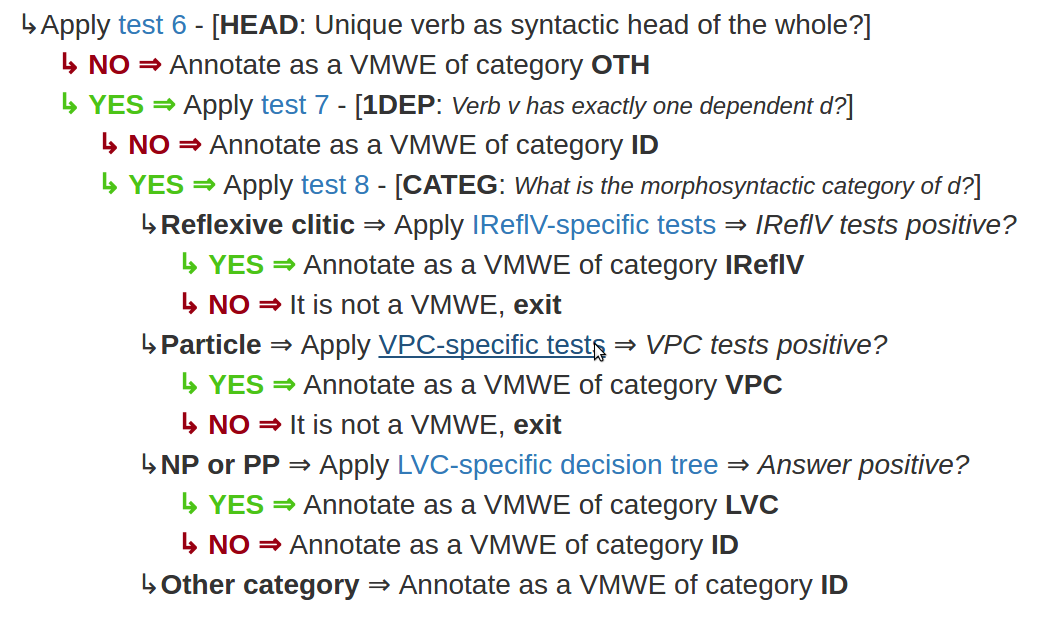
\includegraphics[width=0.8\textwidth]{figures/decision-tree.png}
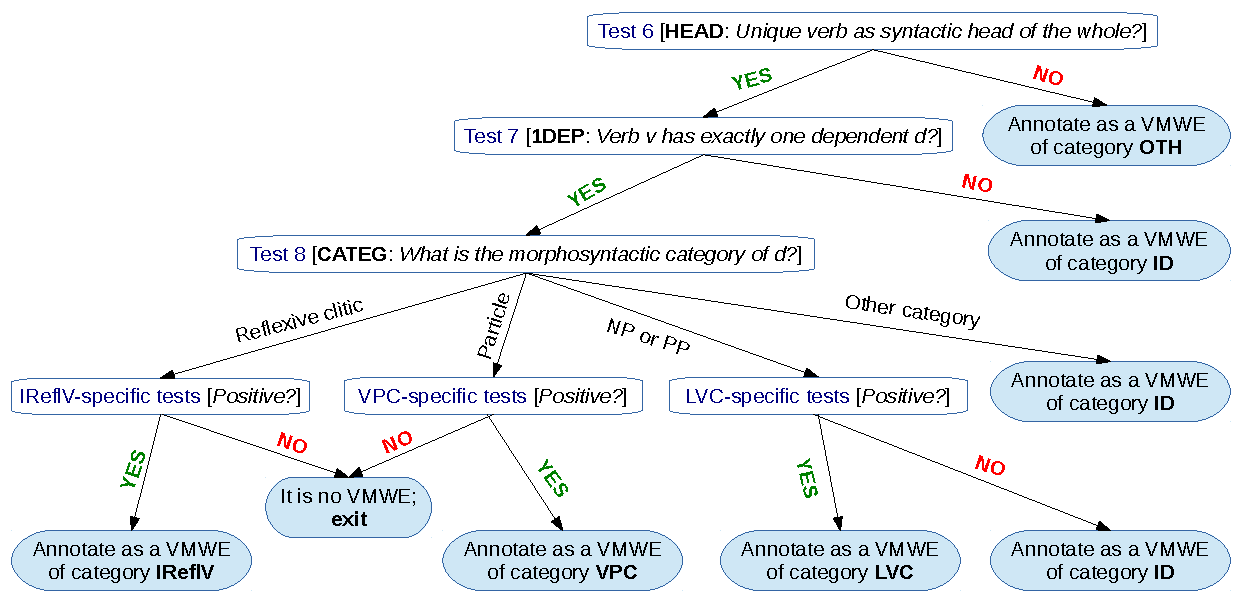
\includegraphics[width=1\textwidth]{figures/decision-tree.pdf}
\caption{Decision tree for VMWE categorisation.}
\label{fig:decision-tree}
\end{figure}

%%%%%%%%%%%%%%%%%%%%%%%%%%%%%%%%%%%%%%%%%%%%%%%%%%%%%%
\subsubsection{Structural tests}
\label{sec:structure}
%\input{chapters/15.structure}
Categorisation of a VMWE %candidate 
depends on the syntactic structure of its canonical form determined by the following three tests\is{verbal multiword expression!structural test}:
\begin{itemize}
\item[]\textbf{Test 6} [HEAD]: Presence of a unique verb functioning as the syntactic head of the whole expression, like in (\ref{fr:laisser-tomber}) 
%FR) \exlitidio{\lex{laisse tomber}}{let fall}{let go} 
and unlike in (\ref{de:leben-und-leben-lassen-2}).
%DE) \exlitidio{wo man \lex{lebt und leben lässt}}{where one lives and lets live}{where one is tolerant}
%(EN) \ile{to \lex{drink and drive}}.%, since there is no universally accepted syntactic representation of coordination. 

\ea \label{fr:laisser-tomber}
\settowidth \jamwidth{(FR)} 
\gll Je \lex{laisse} \lex{tomber}.\\
I let fall \\ \jambox{(FR)}
\glt I let fall. \idio{I let go, I abandon.}
\z

\ea \label{de:leben-und-leben-lassen-2}
\settowidth \jamwidth{(FR)} 
\gll wo man \lex{lebt} und \lex{leben} \lex{lässt} (DE)\\
where one lives and live lets \\
\glt where one lives and lets live \idio{where one is tolerant}
\z

\item[]\textbf{Test 7} [1DEP]: 
%Presence of a unique phrase formed by the lexicalized components and dependent on the head verb, 
Among the phrases dependent on the head verb exactly one contains lexicalised components, 
as in (EN) \ile{\lex{made} it \lex{up}}, and unlike in (EN) \ile{\lex{made up} her \lex{mind}}. 

\item[]\textbf{Test 8} [CATEG]: Morphosyntactic category of the verb's dependent. 
%\cara{changed ``nominal dependent'' to ``verb's dependent'', ok?} 
Contrary to most other tests, the result of this test is not binary but taken from a closed list of values: (i) reflexive clitic (\textsc{refl}), as in (\ref{bg:self-fear}), 
%e.g. (BG) \exlitidio{\lex{страхувам \underline{ce}}}{I fear self}{I am afraid}; 
(ii) particle (\textsc{part}), as in (\ref{de:anfangen});
%e.g.  (DE) \exlitidio{\lex{fängt \underline{an}}}{catches on}{starts};
(iii) nominal or prepositional phrase, as in (\ref{pl:bujac-w-oblokach}); 
%e.g. (PL) \exlitidio{\lex{bujać \underline{w obłokach}}}{to swing in the clouds}{to fantasise}; 
(iv) other (including a verb, an adverb, a non-reflexive pronoun, etc.), as in (\ref{pt:cai-bem}).
%e.g. (PT) \exlitidio{\lex{cai \underline{bem}}}{falls well}{fits}.

\ea \label{bg:self-fear}
\settowidth \jamwidth{(BG)} 
\glll Той \underline{\lex{ce}} \lex{страхува}.\\
toy \underline{\lex{se}} \lex{strahuva} \\
he \textsc{refl} fears \\ \jambox{(BG)}
\glt He fears \textsc{refl}. \idio{He is afraid.}
\z

\ea \label{de:anfangen}
\settowidth \jamwidth{(DE)} 
\gll Der Film \lex{fängt} \underline{\lex{an}}.\\
the film catches \textsc{part} \\ \jambox{(DE)}
\glt The film catches \textsc{part}. \idio{The film begins.}
\z

\ea \label{pl:bujac-w-oblokach}
\settowidth \jamwidth{(PL)} 
\gll Mój bratanek \lex{buja} \underline{\lex{w}} \underline{\lex{obłokach}}.\\
my nephew swings in clouds \\ \jambox{(PL)}
\glt My nephew swings in the clouds. \idio{My nephew fantasizes.}
\z

\ea \label{pt:cai-bem}
\settowidth \jamwidth{(PT)} 
\gll Uma ajudinha \lex{cai} muito \underline{\lex{bem}}. \\
a help.\textsc{dim} falls very well \\ \jambox{(PT)}
\glt A little help falls very well. \idio{A little help  comes at the right moment.}
\z

\end{itemize}

When a VMWE fails Test 6 or 7, it is automatically classified as OTH and ID, respectively. This means that we do not allow cumulative categories. For instance, in (\ref{de:sich-vorstellen})
%(DE) \exlitidio{er \lex{stell dir vor}}{put yourself ahead}{imagine} 
the reflexive clitic considerably changes the meaning of the base VPC from (\ref{de:vorstellen}), 
%\exlitidio{\lex{stell vor}}{put ahead}{present}, 
which might qualify the whole as an IReflV. However, due to the presence of two lexicalised syntactic arguments of the verb, such cases are necessarily classified as IDs (here: with a nested VPC). 

\ea \label{de:vorstellen}
\settowidth \jamwidth{(DE)} 
\gll Er \lex{stellte} mir seine Freundin \lex{vor}.\\
he put me his friend \textsc{part} \\ \jambox{(DE)}
\glt He put his friend \textsc{part} to me. \idio{He presented his friend to me.}
\z

\ea \label{de:sich-vorstellen}
\settowidth \jamwidth{(DE)} 
\gll Er \lex{stellte} \lex{sich} die Reise \lex{vor}. \\
he put \textsc{refl.3.sg} the travel \textsc{part} \\ \jambox{(DE)}
\glt He put the travel \textsc{part} to \textsc{refl}. \idio{He imagined the travel.}
\z

%(DE) \exlitidio{\lex{sich Fragen stellen}}{self questions ask}{to doubt} the reflexive clitic considerably changes the meaning of the base construction \exidio{Fragen stellen}{ask questions}, which might qualify the whole as an IReflV \fc{Not sure this is a good example. I personally do not know this expression, at least not in its plural form. What I can say is "Ich habe mir die Frage gestellt ob das so ist" but it means not "doubt" but rather "wondering".}. 


Test 8, with return values (i)-(iii), triggers the category-specific tests for IReflVs, VPCs and LVCs, respectively. For other categories the candidate automatically qualifies as an ID.

%%%%%%%%%%%%%%%%%%%%%%%%%%%%%%%%%%%%%%%%%%%%%%%%%%%%%%
\subsubsection{Light-verb constructions}
\label{sec:lvcs}
%\input{chapters/15.lvcs}
Light-verb constructions (LVCs)\is{light-verb construction} gave rise to a vast literature since first introduced by \citet{jespersen:65}, possibly because there is no consensus on their exact definition and scope. 
%
We consider a candidate sequence an LVC if it consists of a verb $V$ and a nominal complement $N$, possibly introduced by a preposition, provided that it passes all of the following tests:

\begin{itemize}
\item[] \textbf{Test 9} [N-EVENT]: $N$ denotes an event or a state, as in (\ref{el:have-ability}); %\\e.g. (EL) \ealitidio{\lex{έχουν} τη \lex{δυνατότητα}}{have the ability}{are able}.

\ea \label{el:have-ability}
\settowidth \jamwidth{(EL)}
\glll Οι συσκευές \lex{έχουν} τη \underline{\lex{δυνατότητα}} σύνδεσης.\\
I siskieves eχun ti δinatotita sinδesis \\
the devices have the ability connection.\textsc{sg.ge}.\\ \jambox{(EL)}
\glt The devices have the ability to connect. \idio{The devices can connect.}
\z

\item[] \textbf{Test 10} [N-SEM]: $N$ has one of its original senses, as in (\ref{fr:rendre-visite}) and unlike in (\ref{fr:jetter-eponge});
%like in (FR) \ealitidio{\lex{rend visite}}{returns a visit}{pays a visit} and unlike in (FR) \exlitidio{\lex{jette l'éponge}}{throws the sponge}{gives up}.

\ea \label{fr:rendre-visite}
\settowidth \jamwidth{(FR)}
\gll Steffi \lex{rend} \lex{visite} à Monica. \\
Steffi returns visit to Monica\\ \jambox{(FR)}
\glt Steffi returns a visit to Monica. \idio{Steffi pays a visit to Monica.}
\z

\ea \label{fr:jetter-eponge}
\settowidth \jamwidth{(FR)}
\gll Je \lex{jette} l'\lex{éponge}. \\
I throw the'sponge\\  \jambox{(FR)}
\glt I throw the sponge. \idio{I give up.}
\z

\item[] \textbf{Test 11} [V-LIGHT]: $V$ only contributes morphological features (tense, mo\-od, person, number, etc.) but 
adds no semantics that is not already present in $N$, other than the semantic role of $V$'s subject with respect to $N$, as in (\ref{lt:make-conclusion});
%(PL) \ealitidio{\lex{odniosła sukces}}{carried back a success}{was successful}.

%\ea \label{lt:make-conclusion}
%\settowidth \jamwidth{(LT)}
%\gll Gydytojai \lex{padarė} \lex{išvadą}. \\
%Doctors made conclusion\\ \jambox{(LT)}
%\glt The doctors made a conclusion. \idio{The doctors came to the conclusion.}
%\z

\ea \label{lt:make-conclusion}
\settowidth \jamwidth{(LT)}
\gll Gydytojai \lex{padarė} \lex{išvadą}, kad gijimo procesas vyksta sėkmingai. \\
Doctors made conclusion, that recovery process happens successfully.\\ \jambox{(LT)}
\glt The doctors made the conclusion that the recovery process is successful. \idio{The doctors came to the conclusion that the recovery process is successful.}
\z


\item[] \textbf{Test 12} [V-REDUC]: An NP headed by $N$ can be formed containing all of $V$'s syntactic arguments, and denoting the same event or state as the LVC, e.g. (EN) \ile{Paul \lex{had} a nice \lex{walk}} denotes the same event as (EN) \ile{the nice walk of Paul}. 

\item[] \textbf{Test 13} [N-PROHIBIT-ARG]: A semantic argument of the same type cannot be syntactically realised twice -- both for $N$ and for $V$, e.g. (EN) \ile{*Paul \lex{made} the \lex{decision} \underline{of the committee}} is meaningless, while (EN) \ile{Paul leads the discussion of the committee} is acceptable. Therefore, \ile{to lead a discussion} is not an LVC. %Thus, (EN) \ile{\lex{make} a \lex{decision}} is and \ile{lead a discussion} is not an LVC.
%\cara{Tests 12 and 13 were inverted, but the names were not. Correct now}
    
\end{itemize}

Tests 12 and 13 are syntactic tests approximating the property that one of $V$'s syntactic arguments (generally its subject) is $N$'s semantic argument.

Note that our definition of an LVC does not fully overlap with the state of the art. On the one hand, we are more restrictive than some approaches in that we do not include cases in which the verb does add some (even bleached) semantics to the noun. For instance, inchoative verbs combined with non-inchoative nouns such as (PL) \exlitidio{objąć patronat}{to embrace patronage}{to take on patronage} fail Test 11 and are therefore not classified as LVCs, although their fully bleached counterparts are, as (PL) \exlitidio{\lex{sprawować patronat}}{to perform patronage}{to dispense patronage}. On the other hand, we include in LVCs those combinations in which a semantically void verb selects a large class of action/state nouns so that its lexical non-com\-po\-si\-tio\-na\-li\-ty is hard to establish, e.g. (FR) \ile{\lex{commettre} un \lex{crime}/\lex{délit}/\lex{meurtre}/\ldots} \idio{to commit a crime/offence/murder/\ldots}.

The latter reason makes LVCs belong to the grey area of (non-)com\-po\-si\-tio\-na\-li\-ty. 
%The gray-area cases which we do include in our annotation scope are light-verb constructions. 
They are mostly morphologically and syntactically regular. They can also be seen as semantically %trivially 
compositional in the sense that the semantically void light verb is simply omitted in the semantic calculus. However, this omission %triviality 
may itself be seen as an irregular property. This confirms the observation of \citet{Kracht07} that \isi{compositionality} is a property of linguistic analyses rather than of language items.

%%%%%%%%%%%%%%%%%%%%%%%%%%%%%%%%%%%%%%%%%%%%%%%%%%%%%%
\subsubsection{Idioms}
\label{sec:ids}
%\input{chapters/15.ids}
A verbal idiomatic expression (ID)\is{idiom!verbal} comprises a head verb $V$ (possibly phrasal) and at least one of its arguments. Following the decision tree from \figref{fig:decision-tree}, a VMWE is classified as an ID in one of the 3 cases:
\begin{enumerate}
\item\label{many-lex-arg} $V$ has more than one lexicalised argument, as in (\ref{sl:heart-in-pants}) and (\ref{fa:life-arrived-at-lips})
%\as{Please, check the gloss and provide the transcription};
%e.g. (SL) \exlitidio{\lex{\underline{srce}} mu je \lex{padlo} \lex{\underline{v hlače}}}{his heart fell into his pants}{he lost courage}, 
%(FA) \exlitidio{\PRL{گل بود به سبزه هم آراسته شد}}{there was a flower and now it is also adorned with some green}{a bad situation becomes worse}


\ea \label{sl:heart-in-pants}
\settowidth \jamwidth{(SL)}
\gll \lex{\underline{Srce}} mu je \lex{padlo} \lex{\underline{v}} \lex{\underline{hlače}}. \\
heart him is fallen in pants\\ \jambox{(SL)}
\glt His heart fell into his pants. \idio{He lost courage.}
\z

\ea \label{fa:life-arrived-at-lips}
\settowidth \jamwidth{(FE)}
\glll .\PRL{رسید} \PRL{ـم}\underline{\PRL{لبـ}}  \underline{\PRL{به}}  \PRL{ـم}\underline{\PRL{جانـ}} \\
%\settowidth \jamwidth{()}
%\glll \PRL{رسید} \underline{\PRL{ـم}\PRL{لبـ}} \underline{\PRL{به}} \underline{\PRL{ـم}\PRL{جانـ}}\\
%dʒɒ:næm be læbæm resi:d \\
%soul-my to lips-my arrived\\
%resi:d læbæm be dʒɒ:næm\\
\lex{resid} \lex{lab}am \lex{be} \lex{jan}am\\
arrived lips-my to soul-my\\ \jambox{(FA)}
%\glt my life (being/soul) arrived at my lips (implying `frustration/annoyance’)
\glt My soul arrived at my lips. \idio{I am frustrated.}
\z

%\settowidth \jamwidth{()}
%\glll \lex{\underline{\PRL{شد}}} \underline{\PRL{آراسته}} \underline{\PRL{هم}} \underline{\PRL{سبزه}} \underline{\PRL{به}} \PRL{بود} \underline{\PRL{گل}} (FA)\\
%please, provide the transcription \\
%became adorned and all green was flower\\
%\glt there was a flower and now it is also adorned with some green `a bad situation becomes worse’


%(EN) \ile{\lex{\underline{fortune} favours \underline{the bold}}}.
\item $V$'s single lexicalised argument is of any category other than a reflexive clitic, a particle or a nominal phrase (possibly introduced by a preposition), as in (\ref{pl:dopiac-swego}), (\ref{de:es-gibt}) and (\ref{pt:saber-onde-pisar});
%e.g. (PL) \exlitidio{\lex{dopięła \underbar{swego}}}{buttoned up her own}{fulfilled her plans}, (DE) \exlitidio{\lex{\underline{es} gibt}}{it gives}{there is}, (PT) \exlitidio{\lex{sabe \underbar{onde pisar}}}{knows where to step}{knows how to succeed}.


\ea \label{pl:dopiac-swego}
\settowidth \jamwidth{(PL)}
\gll Platforma \lex{dopięła} \lex{\underline{swego}}. \\
Platform \textsc{part}-buttoned own\\ \jambox{(PL)}
\glt The Platform buttoned \textsc{part} her own. \idio{The Platform fulfilled its plans.}
\z

\ea \label{de:es-gibt}
\settowidth \jamwidth{(DE)}
\gll  \lex{\underline{Es}} \lex{gibt}  kein Zurück.\\
it gives no back\\ \jambox{(DE)}
\glt It gives no retreat. \idio{There is no retreat.}
\z

\ea \label{pt:saber-onde-pisar}
\settowidth \jamwidth{(PT)}
\gll Ele \lex{sabe} \underline{\lex{onde}} \underline{\lex{pisar}}. \\
he knows where step\\ \jambox{(PT)}
\glt He knows where to step. \idio{He knows how to succeed.}
\z

\item\label{id-vs-lvc} $V$'s single lexicalised argument is a nominal phrase (possibly introduced by a preposition), at least one of the  LVC-specific Tests 9--13 fails but at least one of the identification Tests 1--5 applies, as in (\ref{tr:come-to-mind}).
%\as{Please, review the example and provide the idiomatic translation.}

\ea \label{tr:come-to-mind}
\settowidth \jamwidth{(TR)}
\gll Artık kimsenin \lex{aklına} \lex{gelmeyecek}.\\
anymore of-anyone to-his-mind it-will-not-come\\ \jambox{(TR)}
\glt It will not come to the mind of anyone anymore. \idio{No one will remember it anymore.}
\z

\end{enumerate}

Distinguishing an ID from an LVC in case~\ref{id-vs-lvc} is one of the hardest and most frequent annotation challenges.  In case~\ref{many-lex-arg}, care must be taken to identify and also annotate nested VMWEs (if any), e.g. the VMWE in (\ref{ro:reveal-intentions}) 
%(RO) \exlitidio{\lex{dă cărțile pe față}}{gives the cards on face}{reveals one's intentions} 
contains a nested ID (RO) \exlitidio{\lex{dă pe față}}{gives on face}{reveals}. 

\ea \label{ro:reveal-intentions}
\settowidth \jamwidth{(RO)}
\gll El \lex{dă} \lex{cărțile} \lex{pe} \lex{față}. \\
he gives cards on face\\ \jambox{(RO)}
\glt He gives the cards on the face. \idio{He reveals his intentions.}
\z


Idioms whose head verb is the copula (\ile{to be}) pose special challenges because their complements may be (nominal, adjectival, etc.) MWEs themselves. In this task, we consider constructions with a copula to be VMWEs only if the complement does not retain the idiomatic meaning when used without the verb. For instance, (PL) \exlitidio{on \lex{jest jedną nogą na tamtym świecie}}{he is with one leg in the other world}{he is close to death} is an ID because (PL) \exidio{jedna noga na tamtym świecie}{one leg in the other world} loses the idiomatic meaning, while (PL) to stwierdzenie \exlitidio{jest do rzeczy}{this statement is to the thing}{this statement is relevant} is not a VMWE since (PL) \exlitidio{do rzeczy}{to the thing}{relevant} keeps the idiomatic reading.

%%%%%%%%%%%%%%%%%%%%%%%%%%%%%%%%%%%%%%%%%%%%%%%%%%%%%%
\subsubsection{Inherently reflexive verbs}
\label{sec:ireflvs}
%\input{chapters/15.ireflvs}
Pronominal verbs, sometimes also called reflexive verbs, are formed by a verb combined with a reflexive clitic (\textsc{refl}). %For instance, in French the verb \ile{s'apercevoir}{to realize} is formed by the combination of \ile{apercevoir}{see} with reflexive clitic \ile{se}{oneself}. 
They are very common in Romance and Slavic languages, and occur in some Germanic languages such as German and Swedish. Clitics can be highly polysemous and sometimes have an idiomatic rather than a reflexive meaning, in which case we call them inherently reflexive verbs (IReflVs)\is{inherently reflexive verb}. To distinguish regular from idiomatic uses of reflexive clitics, we rely on an IReflV-specific decision tree\footnote{\url{http://parsemefr.lif.univ-mrs.fr/parseme-st-guidelines/1.0/?page=ireflv}} containing 8 tests, which are meant to capture an idiosyncratic relation between a verb with a reflexive clitic and the same verb alone. The first 3 of these tests are sufficient to identify most of the actual IReflVs:

\begin{itemize}
\item[] \textbf{Test 14} [INHERENT]: $V$ never occurs without $C$, as in (\ref{sv:oversleep-self});
%(SV) \exlitidio{\lex{försover sig}}{oversleeps self}{oversleeps};
%(CZ) \exlitidio{\lex{stydí se}}{shames self}{feels ashamed}. 

\ea \label{sv:oversleep-self}
\settowidth \jamwidth{(SV)}
\gll Jonas har \lex{försovit} \lex{sig} idag. \\
Jonas has overslept \textsc{refl.3.sg} today\\ \jambox{(SV)}
\glt Jonas overslept \textsc{refl} today. \idio{Jonas overslept today.}
\z

\item[] \textbf{Test 15} [DIFF-SENSE]: $C$ markedly changes the meaning of $V$, as in (\ref{sl:tice-se});
%(SL) \exlitidio{\lex{tíče se}}{refers self}{concerns}


\ea \label{sl:tice-se}
\settowidth \jamwidth{(SL)}
\gll kar \lex{se} \lex{tiče} Kosova \\
what \textsc{refl} touches Kosovo\\ \jambox{(SL)}
\glt what \textsc{refl} touches Kosovo \idio{as far as Kosovo is concerned}
\z

%(SV) \exlitidio{\lex{känner sig} ledsen}{touches self sad}{feels sad}.% vs. \exidio{apercevoir}{perceive}. 
\item[] \textbf{Test 16} [DIFF-SUBCAT]: $C$ changes the subcategorisation frame of $V$, as in (\ref{pt:self-forget}) vs.
%(PT) \exlit{X \lex{se esqueceu} de Y}{X self forgot of Y} 
(PT) \exlit{você me esqueceu}{you forgot me}.


\ea \label{pt:self-forget}
\settowidth \jamwidth{(PT)}
\gll Você \lex{se} \lex{esqueceu} de mim. \\
you \textsc{refl.3.sg} forgot of me\\ \jambox{(PT)}
\glt You forgot \textsc{refl} about me. \idio{You forgot about me.}
\z

\end{itemize}

IReflVs are hard to annotate because pronominal clitics have several different uses. %, and annotators must distinguish IPronVs from other uses. 
For example, %the REFL clitic 
(IT) \exidio{si}{\textsc{refl}} can occur not only in IReflVs such as (IT) \exlitidio{\lex{riferir}\lex{si}}{to report.\textsc{refl}}{to refer}, but also 
in the following non-idiomatic cases: reflexive (IT) \exidio{lavarsi}{to wash.\textsc{refl}}, possessive reflexive (IT) \ile{grattarsi la testa} \litidio{to scratch.\textsc{refl} head}{to scratch one's head}, reciprocal (IT) \exlit{baciarsi}{to kiss.\textsc{refl}} $\Rightarrow$\idio{to kiss each other}, impersonal (IT) \exlitidio{si dorme molto}{\textsc{refl} sleeps much}{people sleep a lot},  middle alternation (IT) \exlitidio{si affittano case}{\textsc{refl} rent houses}{houses are rented} or inchoative (IT) \exlitidio{la porta si apre}{the door \textsc{refl} opens}{the door opens}. 
%A dedicated decision tree,\footnote{\url{http://parsemefr.lif.univ-mrs.fr/parseme-st-guidelines/1.0/?page=ireflv}} with the above Tests 14--16 and Tests 17--21 (not cited here) and multilingual examples, allows us to distinguish IReflVs from other uses. 
%Nevertheless, this
The IReflV category was reported as the most challenging to annotate by some teams, notably the Spanish and the Romanian ones.

%%%%%%%%%%%%%%%%%%%%%%%%%%%%%%%%%%%%%%%%%%%%%%%%%%%%%%
\subsubsection{Verb-particle constructions}
\label{sec:vpcs}
%\input{chapters/15.vpcs}
Verb-particle constructions (VPCs)\is{verb-particle construction} are pervasive notably in Germanic languages and Hungarian, but virtually non-existent in Romance or Slavic languages. They are formed by a lexicalised head verb $V$ and a lexicalised particle $P$ dependent on $V$, whose joint meaning is non-compositional. The latter property is approximated by a unique syntactic test:

%\capa{Not sure, but I seem to recall that Italian was also including them in the annotation guidelines. If that is the case maybe non-existent for all Romance languages is wrong?}
%\as{In Italian VPCs are actually mainly understood as prepositional verbs.}

\begin{itemize}
\item[] \textbf{Test 22} [V+PART-DIFF-SENSE] A sentence without $P$ does not refer to the same event/state as the sentence with $P$.  For example, the sentence in (\ref{hu:bump-on})
%(HU) \exlitidio{\lex{be}|\lex{jött} ez a koktél nekem}{this coctail bumped on into me}{I like this coctail} 
does not imply (HU) \exidio{nekem jött ez a koktél}{this cocktail bumped into me}, while (DE) \exidio{er legt das Buch auf dem Tisch ab}{he puts the book on the table \textsc{part}} implies (DE) \exidio{er legt das Buch auf dem Tisch}{he puts the book on the table}. 


\ea \label{hu:bump-on}
\settowidth \jamwidth{(HU)}
\gll  \lex{Be}-\lex{jött} ez a koktél nekem. \\
\textsc{part}-bumped this the cocktail for.me\\ \jambox{(HU)}
\glt This cocktail bumped \textsc{part} into me. \idio{I like this cocktail.}
\z

\end{itemize}

The first challenge in identifying a VPC is to distinguish a particle, as in (EN) \ile{to \lex{get \underbar{up}} a party},  from a homographic preposition, as in (EN) \ile{to get \underbar{up} the hill}. Language-specific tests were designed for German and English to this aim.

In some Germanic languages and also in Hungarian, verb-particle constructions can be spelled either as one (multiword) token, as in (\ref{hu:kick-in-1}), 
%e.g.  (HU) \exlitidio{\lex{be}|\lex{rúgott}}{in-kicked}{got drunk}, 
or separated, as in (\ref{hu:kick-in-2}). %\as{Please, check the glosses.}
%e.g. (HU) \exlitidio{nem \lex{rúgott be}}{did not kick in}{did not get drunk}. 
Both types of occurrences are to be annotated.


\ea \label{hu:kick-in-1}
\settowidth \jamwidth{(HU)}
\gll  ő \lex{be}-\lex{rúgott}. \\
he \textsc{part}-kicked\\ \jambox{(HU)}
\glt He kicked \textsc{part}. \idio{He got drunk.}
\z

\ea \label{hu:kick-in-2}
\settowidth \jamwidth{(HU)}
\gll Nem ő \lex{rúgott} \lex{be}. \\
not he kicked \textsc{part}\\ \jambox{(HU)}
\glt He did not kick \textsc{part}. \idio{He did not get drunk.}
\z

Special care must be taken with polysemous constructions having both a compositional and a non-compositional reading, as in (DE) \exidio{ein Schild aufstellen}{to put up a sign}  vs. (DE) \exlitidio{einen Plan \lex{auf}\lex{stellen}}{to put up a plan}{to draw up a plan}.

%%%%%%%%%%%%%%%%%%%%%%%%%%%%%%%%%%%%%%%%%%%%%%%%%%%%%%
\subsubsection{Other VMWEs}
\label{sec:oth}
%\input{chapters/15.oth}
This category gathers the VMWEs which do not have a single verbal head (cf. Test 6 in \figref{fig:decision-tree} and \sectref{sec:structure}). Those include:
\begin{itemize}
\item Coordinations like in example (\ref{de:leben-und-leben-lassen-2}) p.~\pageref{de:leben-und-leben-lassen-2}, or (\ref{he:carry-and-give})
%\as{Please, check the gloss and provide the transcription};
%(DE) \exlitidio{wo man \lex{lebt und leben lässt}}{where one lives and lets live}{where one is tolerant} and 
%(HE) \exlitidio{\lex{יעבור} \lex{ואל} \lex{יהרג}}{will be killed and will not pass}{something is allowed under no circumstances}

%\ea \label{he:kill-not-pass}
%\settowidth \jamwidth{(HE)}
%\glll .\lex{יעבור} \lex{ואל} \lex{יהרג} \lex{הוא} \lex{הנושא} \\
%\lex{ya'vor} \lex{veal} \lex{yehareg} \lex{hu} hanose \\ 
%will.pass and.not will.be.killed is the.subject\\ \jambox{(HE)}
%\glt The subject is to be killed and not to pass. \idio{The subject is allowed under no circumstances.}
%\z

\ea \label{he:carry-and-give}
\settowidth \jamwidth{(HE)}
\glll .\textup{מצרים} \textup{עם} \lex{ונתנה} \lex{נשאה} \textup{בריטניה} \\
%\glll .עם מצרים \\%\lex{ונתנה} \lex{נשאה {בריטניה \\ 
micrayim 'im \lex{ve-natna} \lex{nas'a} britanya \\ 
Egypt with and-gave carried Britain\\ \jambox{(HE)}
\glt Britain carried and gave with Egypt. \idio{Britain negotiated with Egypt.}
\z

%(PL) \exlitidio{coś kogoś \lex{ani ziębi, ani grzeje}}{sth neither cools nor warms someone}{someone is indifferent to sth};
\item Compound verbs, resulting usually from conversion of nominal com\-po\-unds, and therefore having no regular verbal structure, as in (\ref{fr:court-circuiter}) or in 
%(FR) \exidio{\lex{court-circuitera}}{will short-circuit}, 
(EN) \ile{to \lex{pretty-print}}. 


\ea \label{fr:court-circuiter}
\settowidth \jamwidth{(FR)}
\gll On \lex{court-circuite} le réseau terrestre. \\
one short-circuits the network terrestrial \\ \jambox{(FR)}
\glt One short-circuits the terrestrial network. \idio{One bypasses the terrestrial network.}
\z

\end{itemize}

%%%%%%%%%%%%%%%%%%%%%%%%%%%%%%%%%%%%%%%%%%%%%%%%%%%%%%
\subsection{Language-specific interpretation of the guidelines}
\label{sec:lang-spec-guide}
%\input{chapters/15.lang-spec-guide}
Despite huge efforts put into setting up generic terminologies and methodologies, as well as into the pilot annotations and the project coordination, language-specific interpretation of the final guidelines could not be avoided. This was mainly due to different linguistic sensitivities and traditions, language-specific challenges and incompleteness or imprecision of the guidelines.

The most notable deviation occurred in Farsi\il{Farsi}, where no categorisation was performed, and the OTH label was used for all identified VMWEs instead. The main reason is the particularly challenging nature of the VMWE phenomenon in this language. There are less than 200 actively used simple (single-word) verbs, and a large majority of events and processes are expressed by multiword combinations, many of which are potential VMWEs. 
The implications on our annotation process are at least threefold. Firstly, verbs are extremely polysemous, so Test 11 (\sectref{sec:lvcs}) is very difficult to apply. In particular, 
the highly frequent light verb \nlile{\PRL{کردن}}
\exidio{/kardan/}{to do/make} is ambiguous in its passive form  \nlile{\PRL{شدن}}\exidio{/šodan/}{done/made} with the semi-copula equivalent roughly to \idio{become}. Only the former interpretation should yield a VMWE annotation but the difference is hard to capture.  
Secondly, rephrasing an LVC by a single verb, often used to approximate Test 9 in other languages (\ile{to \lex{make} a \lex{decision}} = \ile{to decide}), is rarely feasible in Farsi. Thirdly, VMWEs are extremely pervasive, which is easily visible in \tabref{tab:corpora-overview}: the number of annotated VMWEs is roughly the same as the number of sentences, i.e.\ almost every main verb is the head of a VMWE. As a result, the VMWE phenomenon is particularly hard to capture in Farsi since it can rarely be contrasted  with verbal constructions deemed compositional.

Another notable deviation occurred in Slovene\il{Slovene}, where the VPC category, as defined by the generic guidelines, hardly or never occurs, however it was used instead to annotate idiomatic verb-preposition combinations, such as  (SL) \exlitidio{\lex{prišlo} je \lex{do} nesreče}{it came to an accident}{an accident occurred}. 

%(HE) \exidio{\lex{לאזורי} \lex{הודות}}{thanks to-the-areas-of}, 
%the free complement \exidio{אזורי}{areas-of} had to be annotated as lexicalised together with its governing preposition \exidio{ל}{to}.

%instead of the more plausible one: (HE) \ile{אזורי}\lex{ל} \lex{הודות}}, where only the preposition would but not the free complement \exidio{אזורי}{areas} would considered lexicalized in the last (left-most) token.

The status of VPCs in Italian\il{Italian} is interesting. As a Romance language, Italian was expected not to exhibit VPCs, but several dozens of VPC annotations do occur in the Italian corpus, e.g.\ (IT) \exlitidio{\lex{volata via}}{flew \textsc{part}}{slipped away}, %\jm{I would rather prefer the meaning of 'slipped away'for volata via}.,
\exlitidio{\lex{tira fuori}}{pulls \textsc{part}}{shows}, 
%\jm{I would rather prefer the meaning of 'shows'}, 
or \exlitidio{\lex{va avanti}}{goes \textsc{part}}{goes on}. This shows the possibly ambiguous status of \exidio{via}{by/away}, \exidio{avanti}{on/forward}, \exidio{fuori}{out/out\-side}, etc.\ as either adverbs or particles, triggering the ID or the VPC category, respectively. The semantic compositionality of some of these constructions might also be examined more closely.

In Bulgarian\il{Bulgarian} and Czech\il{Czech}, the auxiliaries accompanying the head verbs were annotated as VMWE components, e.g.\ in (CS) \exlitidio{on \lex{se} \underline{bude} \lex{bavit}}{he \textsc{refl} \underline{will} play}{he will play}, in (BG) %\exlit{те не \lex{\underline{са} дали} \lex{съгласие}}
\exlit{te ne \underline{sa} \lex{dali saglasie}}{they not \underline{are} given consent} $\Rightarrow$\idio{they have not given consent}. This is in contrast with the guidelines, which stipulate that only the lexicalised components should be annotated. % (although the case of auxiliaries is not explicitly mentioned). 
The motivation for this deviation was to always include a finite verb in the annotated expression, so as to e.g.\ easily study the tense and mood restrictions in VMWEs. Since such studies are enabled by the accompanying morpho-syntactic data (currently existent in Czech and to be provided in Bulgarian in the future), these divergences should be eliminated in new editions of the corpus. 

%\as{I'm not sure of this paragraph. Fabienne, please, check.} 
In German\il{German}, a deviation was observed with respect to VMWEs containing both a reflexive clitic and a particle such as  (DE) \exlitidio{sie \lex{bringen sich ein}}{they bring \textsc{refl} \textsc{part}}{they contribute}. Such cases were annotated as IReflVs with nested VPCs, which does not conform to Test 7 (\sectref{sec:structure}) stipulating that, whenever the VMWE has more than one lexicalised dependent of the head verb, it should be classified as an ID (here: with a nested VPC).  Good reasons exist for each of these strategies and more discussion is needed to arbitrate for future releases of the guidelines.

Lithuanian\il{Lithuanian} seems to have a surprisingly low number of LVCs, despite the large size of the annotated corpus. It would be worthwhile to study in more detail if this phenomenon is inherent to the language or results from a more restrictive understanding of the LVC scope.

In Hebrew\il{Hebrew}, a relatively large number of VMWEs of type OTH was observed (cf. \tabref{tab:corpora-overview}), and a necessity of defining a new category (specific to non-Indo-European languages) was hypothesised. A more detailed study revealed that most OTH annotations were spurious: they concerned statistical collocations or VMWEs of the ID or LVC types. Some idiomatic verb-preposition combinations were also annotated in Hebrew\il{Hebrew}, despite the fact that we had abandoned the IPrepV category in the earlier stages of the project (\sectref{sec:typology}). There, the annotators faced a particular challenge from prepositions which often attach to the governed noun and annotating them as separate lexicalised tokens was mostly impossible. Thus, in the following sequence: 
(HE) %\nlexidio{אבטלה \lex{מאחוז} \lex{סובל}}
\exidio{sovel me.achuz avtala}{suffers from.a.percentage of.unemployment} the free complement %\nlexidio{אחוז}
\exidio{achuz}{percentage} had to be annotated as lexicalised together with its governing preposition %\nlexidio{מ}
\exidio{me}{from}. This problem will be dealt with in the future, when inherently adpositional verbs will be addressed (\sectref{sec:conclusions}).

In Turkish\il{Turkish}, the LVC and OTH types also had their language-specific interpretation. Namely, the Turkish PARSEME corpus resulted from adapting a pre-existing MWE typology and dataset \citep{ciclingkubra}. There, the definition of a light verb, based on Turkish linguistic works \citep{siemieniec2010some}, was context-independent, i.e.\ restricted to a closed list of 6 verbs: \exidio{olmak}{to be}, \exidio{etmek}{to do}, \exidio{yapmak}{to make}, \exidio{kılmak}{to render}, \exidio{eylemek}{to make} and \exidio{buyurmak}{to order}. Verb-noun combinations with other operator verbs, such as \exlitidio{\lex{söz vermek}}{promise to give}{to promise}, were then classified as OTH. A closer look at the existing OTH annotations reveals, indeed, that most of them can be re-classified as LVC in future releases of the corpus.

Czech\il{Czech} is another language in which a pre-existing MWE-annotated corpus \citep{pdt2017} was adapted to the needs of the PARSEME initiative. There, complex identification and conversion procedures had to be designed \citep{biblio:BeHaExtractingVerbal2017}. 
%\eb{\sout{, notably for IReflVs \citep{DBLP:conf/mwe/UresovaBH16}} No need to cite the second publication; IReflVs were not the main thing, just one we described in detail for this workshop.}. 
The resulting mapping procedure could be fully automatic, which suggests that the understanding of the VMWE phenomenon is similar in both annotation projects. It would still be interesting to compare both annotation guidelines more thoroughly and look for possible divergences.

%%%%%%%%%%%%%%%%%%%%%%%%%%%%%%%%%%%%%%%%%%%%%%%%%%%%%%%%%%%%%%%%%%%%%%%%%%%%%%%%%%%%%%%%%%%%%%%%%%%%%%%%%%%%%%%%%%%%%%%%%%%%%%%%%%%%%%%%%%%%%%%%%%%%%%%%%%%%%%%%%%%%%%%%%%%%%%%%%%%%%%%%%%%%%%%%%%%%%%%%%%%%
%%%%%%%%%%%%%%%%%%%%%%%%%%%%%%%%%%%%%%%%%%%%%%%%%%%%%%%%%%%%%%%%%%%%%%%%%%%%%%%%%%%%%%%%%%%%%%%%%%%%%%%%%%%%%%%%%%%%%%%%%%%%%%%%%%%%%%%%%%%%%%%%%%%%%%%%%%%%%%%%%%%%%%%%%%%%%%%%%%%%%%%%%%%%%%%%%%%%%%%%%%%
\section{Annotation methodology and tools}
\label{sec:methodology}

%\subsection{Annotation challenges}
%\label{sec:challenges}
%\input{chapters/15.challenges}
%Among the challenging features of linguistic annotation, as defined by \citet{DBLP:journals/coling/MathetWM15}, the VMWE annotation task  is concerned by:
\citet{DBLP:journals/coling/MathetWM15} mention several challenging features of linguistic annotation, some of which are relevant to the VMWE annotation task:
%The VMWE annotation process if twofold: 
%In particular, a VWE annotation may contain:
\begin{sitem}
\item \emph{Unitising}, i.e.\ identifying the boundaries of a VMWE in the text;
\item \emph{Categorisation}, i.e.\ assigning each identified VMWE to one of the pre-de\-fined categories (\sectref{sec:typology});%\eb{was Section~\ref{sec:annotation}, please, check.}).
\item \emph{Sporadicity}, i.e.\ the fact that not all text tokens are subject to annotation (unlike in part-of-speech annotation, for instance);
%\end{sitem}
%These are challenging notably because a VMWE can exhibit:
%\begin{sitem}
\item \emph{Free overlap}, e.g.\ in (CS) \exidio{\lex{ukládal} různé \lex{sankce} a \lex{penále}}{put various sanctions and penalties}, where two LVCs share a light verb;

%(EN) \ile{\underline{\lex{take}} a \lex{walk} and then a long \lex{shower}}: 2 LVCs with a shared light verb;
%\item \as{\sout{Embeddings (to avoid confusion with word embeddings)}
\item \emph{Nesting}, 
    \begin{sitem}
    \item at the syntactic level, as in (\ref{pl:skarzyc-sie}), where an IReflV (PL) \exlitidio{\lex{skarżyć się}}{to complain \textsc{refl}}{to complain} occurs in a relative clause modifying the predicative noun of the LVC (PL) \exidio{\lex{popełnić oszustwo}}{to commit a fraud}.
%    e.g. (PL) \exlitidio{\lex{oszustwa}, na jakie \lex{\underline{skarżą się}} Cyganie, \lex{popełniły} grupy zorganizowane}{frauds about which the Gypsies \ul{self complain} committed organised groups}{frauds which Gipsies complain about were committed by organised groups}

\ea \label{pl:skarzyc-sie}
\settowidth \jamwidth{(PL)}
\gll \lex{Oszustwa}, na jakie \lex{\underline{skarżą}} \lex{\underline{się}} Cyganie, \lex{popełniły} grupy zorganizowane. \\
frauds, on which complain \textsc{refl} Gypsies, committed groups organised\\ \jambox{(PL)}
\glt Organised groups committed frauds about which the Gypsies \textsc{refl} complain. \idio{Frauds which Gipsies complain about were committed by organised groups.}
\z

%\ile{\lex{take} the fact that I didn't \underline{\lex{give up}} \lex{into account}}) 
	\item at the level of lexicalised components, as in (\ref{pt:take-into-hands}), where the ID (PT) \exlitidio{\lex{fazer justiça}}{to make justice}{to do justice} is nested within a larger ID.
    %e.g.\ (PT) \exlitidio{\lex{eles \ul{fizeram justiça} com as próprias mãos}}{\ul{ justice} with their own hands}{take the law into their own hands}.%\ile{\lex{\underline{let} the cat \underline{out} of the bag}}).
    

\ea \label{pt:take-into-hands}
\settowidth \jamwidth{(PT)}
\gll Ales \lex{fizeram} \lex{justiça} \lex{com} \lex{as} \lex{próprias} \lex{mãos}. \\
they made justice with their own hands\\ \jambox{(PT)}
\glt They made justice with their own hands. \idio{They took the law into their own hands.}
\z

    \end{sitem}
\end{sitem}
Two other specific challenges are:
\begin{sitem}
\item \emph{Discontinuities}, e.g.\ (CS) \exidio{on \lex{ukládal} \underline{různé} \lex{sankce}}{he put various sanctions};
%(e.g.\ \ile{\lex{take} this \lex{into account}});
\item \emph{Multiword token} VMWEs, e.g.\ separable IReflVs or VPCs:\footnote{Note that annotating separate syntactic words within such tokens would be linguistically more appropriate, and would avoid bias in inter-annotator agreement and evaluation measures -- cf. \sectref{sec:iaa} and \citep{MWEWorkshop}. However, we preferred to avoid token-to-word homogenising mainly for the reasons of compatibility. Namely, for many languages, pre-existing corpora were used, and we would like VMWE annotations to rely on the same tokenisation as the other annotation layers.}\\ (ES) \exlitidio{\lex{abstener}.\lex{se}}{to abstain.\textsc{refl}}{to abstain},\\ (HU) \exlitidio{\lex{át}.\lex{ruház}}{to \textsc{part}.dress}{to transfer}.%
%(DE) \exlitidio{\lex{auf}|\lex{machen}}{out|make}{open}.

%\fc{changed the second reference in footnote to analysis chapter it pointed to "measures" but this label was not defined, someone please check.}
\end{sitem}

\noindent
This complexity is largely increased by the multilingual nature of the task, and calls for efficient project management and powerful annotation tools. 

%%%%%%%%%%%%%%%%%%%%%%%%%%%%%%%%%%%%%%%%%%%%%%%%%%%%%%
\subsection{Project management}
\label{sec:management}
%\input{chapters/15.management}
The list of language teams having initially expressed their interest in this initiative included those mentioned in p.~\pageref{language-groups}, as well as English, Croatian and Yiddish, for which no corpus release could be achieved due to the lack of sufficiently available native annotators. All languages were divided into four language groups (LGs) - Balto-Slavic, Germanic, Romance and others - as also described in p.~\pageref{language-groups}. 
%
The coordination of this large project included the definition of roles -- project leaders, technical experts, language group leaders (LGLs), language leaders (LLs) and annotators -- and their tasks.

The biggest challenge in the initial phase of the project was the development of the annotation guidelines\footnote{Their final version, with examples in many participating languages, is available under the CC BY 4.0 license at %{\scriptsize
\url{http://parsemefr.lif.univ-mrs.fr/parseme-st-guidelines/1.0/}.} which would be as unified as possible but which would still allow for language-specific categories and tests. To this end, a two-phase pilot annotation in most of the participating languages was carried out. Some corpora were annotated at this stage not only by native but also by near-native speakers, so as to promote cross-language convergences. Each pilot annotation phase provided feedback from annotators, triggered discussions among language (group) leaders and organisers, and led to enhancements of the guidelines, corpus format and tools. 

We also defined strategies for selecting the final corpora. They should: (i) be written in the original, 
%\eb{missing `language'?}\as{"in the original" is correct according to \url{http://www.oxfordlearnersdictionaries.com/definition/english/original_2}}
 in order to avoid  MWE-related translationese issues; (ii) correspond to the same genre: newspaper texts or Wikipedia articles;\footnote{Deviations from this rule occurred in some languages due to the choice of pre-existing corpora, e.g. in Hungarian legal texts were used.} (iii) consist of longer text fragments (rather than isolated sentences), so as to enable disambiguation and coreference resolution; (iv) not be automatically pre-selected in view of a higher density of VMWEs (so as to provide both positive and negative examples); (v) be free from copyright issues, i.e.\ compatible with open licenses. 

%%%%%%%%%%%%%%%%%%%%%%%%%%%%%%%%%%%%%%%%%%%%%%%%%%%%%%
\subsection{Annotation platform}
\label{sec:flat}
%\input{chapters/15.flat}
For this large-scale corpus construction, we needed a centralised web-based annotation tool. Its choice was based on the
following criteria: (i) handling different alphabets; (ii) accounting for right-to-left scripts; and (iii) allowing for
discontinuous, nested and overlapping annotations. We chose
FLAT\is{FLAT},\footnote{\scriptsize\url{https://github.com/proycon/flat}} a web platform which, in addition to the required criteria, enables token-based selection of text spans,
including cases in which adjacent tokens are not separated by spaces. It is possible to authenticate and manage
annotators, define roles and fine-grained access rights, as well as customise specific settings for different languages.

FLAT is implemented as a web-based frontend with support for multiple users, user groups, and with configurable access rights. The frontend communicates with the FoLiA document server
backend,\footnote{\scriptsize{\url{https://github.com/foliadocserve}}} which loads and holds documents in memory as they are being edited, writes them to disk again at convenient times, and unloads them when they are not used anymore. The document server has Git version control support,\footnote{\scriptsize{\url{https://git-scm.com/}}} allowing changes to be tracked. In addition, for each individual FoLiA annotation, % in a document
e.g.\ each VMWE, %associated 
information  such as who made the annotation, and when, is automatically registered.
%. FLAT fills this annotator information automatically based on the logged in user.
%\as{By MAARTEN: describe the general features of the tool, show a screenshot, list the features added for PARSEME}

%FLAT is a document-centric annotation tool %that 
%aims to provide the ability to annotate using the 
FLAT is document-centric, i.e.\ it supports annotation of full documents together with their structure  (headers, bulleted lists, figures, etc.). 
%typically allows annotators to work on full documents, and supports visualization of full document structure (e.g. headers, figures, bulleted lists, even figures). 
This %can be contrasted to 
contrasts with tools which take a more corpus-based approach with keyword-in-context visualisation. FLAT does allow for various other \emph{perspectives} on 
%Stella's remarks: perspectives of, but see: https://www.oxfordlearnersdictionaries.com/definition/english/perspective?q=perspective
the document; for the PARSEME annotation task a sentence-based perspective was chosen, presenting users with one or more pages of clearly delimited sentences to annotate. An example is shown in \figref{fig:flat1}.

\begin{figure}
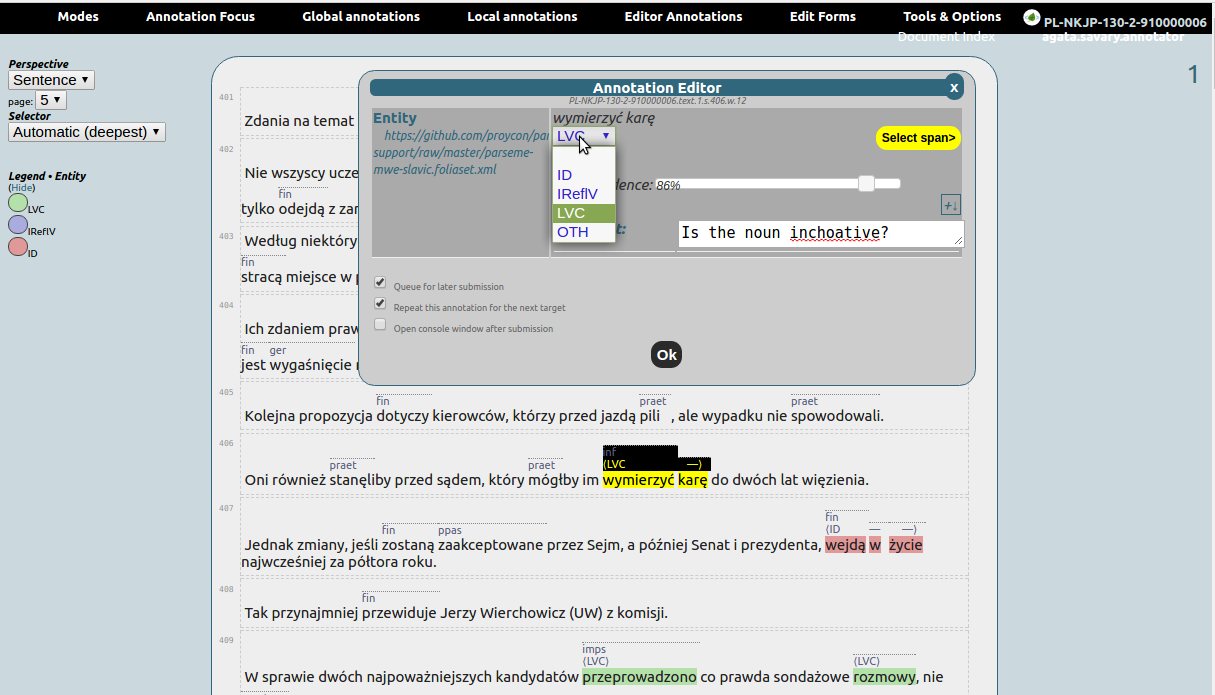
\includegraphics[width=0.98\textwidth]{figures/flat-pl.png}
\caption{FLAT annotation interface with a Polish text. The VMWEs are coloured according to their categories. POS tags (\textit{fin}, \textit{ger}, \textit{imps}, \textit{ppas}, and \textit{praet}) are displayed above all verbal tokens. Some attributes (VMWE category, confidence level and a comment) of the highlighted VMWE (PL) \exlitidio{\lex{wymierzyć karę}}{to \textsc{part}.measure a punishment}{to mete out a punishment} are edited in the annotation editor.}
\label{fig:flat1}
\end{figure}

FLAT is based on FoLiA\is{FoLiA},\footnote{\scriptsize\url{https://proycon.github.io/folia}} a rich XML-based format for linguistic annotation
\citep{GompelReynaert13}, and is compatible with a wide variety of linguistic annotation types. 
VMWEs, or entities as they are called more generically in FoLiA, constitute the most important
annotation type for PARSEME. Still, certain language teams worked on documents enriched with more linguistic
annotations, such as part-of-speech tags, to aid the annotation process, as shown in \figref{fig:flat1}. The underlying aspiration of both FoLiA and
FLAT is to provide a single unified solution for multiple annotation needs, with respect to the encoding format and the 
annotation environment, respectively.



%A characteristic of the FoLiA format is that it 
While the FoLiA format %strictly 
specifies possible linguistic annotation types and structural types, 
it does not commit to any particular tagset/vocabulary nor language. %In fact
Instead, tagsets are
defined externally in \emph{FoLiA set definitions}, which can be published anywhere online by
anyone and are deliberately separate from the annotation format itself. A dozen of set definitions for PARSEME, based on the VMWE categories relevant to different languages or language groups (\sectref{sec:typology}) are likewise published in a public repository.\footnote{\scriptsize{\url{https://github.com/proycon/parseme-support}}} All FoLiA documents declare which particular set definitions to use for which annotation
types. FLAT uses these set definitions to populate various selection boxes,  %with all the tag options the user may select, 
as shown in \figref{fig:flat1}.

%\mvg{MAYBE TODO: screenshot of a MWE selection pull-down list?}\as{Do you mean what is already in Fig.~\ref{fig:flat1}?}\mvg{Exactly, I think the one there is perfect and conserves space, so need need for another one, I referenced it above}

All software discussed here %in this section 
is %freely 
available under an open-source license.\footnote{\scriptsize{GNU Public License v3}} It is %can be considered 
part of a wider and growing infrastructure of FoLiA-capable NLP tools \citep{Gompel_etal:17}, developed and funded in the scope of the %larger
CLARIAH\footnote{\scriptsize{\url{https://www.clariah.nl}}} project and its predecessor CLARIN-NL.

Although FLAT has been in use for various other annotation projects, the PARSEME initiative, currently with over 80 active FLAT users, % in 16 languages
is the biggest use case to
date, and as such has had a very positive influence in terms of the maturity of the software, fixing bugs, attaining improved
performance and scalability, and compiling appropriate documentation. 
%\mvg{NOTE TO EDITOR: if the section gets too long, you may want to omit the following part on features implemented specifically for PARSEME, as it may be too detailed}
Various features were added to accommodate PARSEME specifically: (i) uploading documents in non-FoLiA formats, needed for the parseme-tsv format (\ref{sec:format}); (ii) right-to-left support necessary for Farsi and Hebrew; (iii) a metadata editor; (iv) enhanced file and user management; (v) confidence level and free-text comments as part of the editable attributes (\figref{fig:flat1}).

Out of 18 language teams which achieved a corpus release, 13 used FLAT as their main annotation environment. The 5 remaining teams either used other (generic or in-house) annotation tools, or converted existing VMWE-annotated corpora. 

%%%%%%%%%%%%%%%%%%%%%%%%%%%%%%%%%%%%%%%%%%%%%%%%%%%%%%
\subsection{Automatic VMWE pre-annotation}
\label{sec:pre-annot}
%\input{chapters/15.pre-annot}
Automatic pre-annotation\is{pre-annotation} of corpora is a current practice in many annotation tasks. In the PARSEME corpus project, it was applied by the Bulgarian and Hungarian teams, on the basis of manually compiled lists of VMWEs. All texts were then manually checked and corrected.

More precisely, pre-annotation in Bulgarian included automatic annotation of: (a) verb forms (triggers for VMWEs), (b) IReflV candidates consisting of a verb and a reflexive particle, and (c) VMWEs from a large dictionary of Bulgarian MWEs \citep{Koeva2016}. Cases of false positives included: (i) literal uses of existing VMWEs, (ii) false IReflVs which are true reflexive or passive constructions instead (\sectref{sec:ireflvs}), or (iii) coincidental co-occurrence of VMWE components. All annotations were manually verified and such cases were eliminated. False negatives could also be efficiently tracked thanks to the highlighted verb forms.
%\as{Did you also manually check the false negatives? IS: Annotators were advised to check all verbs (they all were tagged after the POS tagging) for their possible inclusion in VMWEs, so yes, many new MWEs were annotated that were not in the dictionary. Also, they read the whole text in order to discover any derivatives - nouns, adjectives, etc. (e.g., heart broken) - these were also a very small number.}

Automatic pre-annotation is known to introduce a task-dependent bias \citep{Marcus:1993:BLA:972470.972475,Fort:2010:IPP:1868720.1868727} which may be both positive (simple repetitive tasks are handled uniformly and speeded up) and negative (annotators may tend to rely too much on the automatic pre-annotation and fail to detect false negatives). We are not aware of any studies about biases related to VMWE annotation. We expect a minor risk of bias to stem from a possibly unbalanced VMWE dictionary: if one category (e.g.\ LVCs) is better represented than others, annotators may become more attentive to it. A bias might also be introduced by relatively productive constructions, when a large majority, but not all, of their occurrences belong to a unique category. For instance, the verb (BG)
% \nlexidio{давам}
\exidio{davam}{to give} occurs often and in many different LVCs, e.g.\ with %\nlexidio{съгласие}
\exidio{saglasie}{consent}, %\nlexidio{разрешение}{permission},
\exidio{razreshenie}{permission} %\nlexidio{обяснение}{explanation}
\exidio{obyasnenie}{explanation}, etc. The annotators could, therefore, tend to wrongly assign the LVC category to other expressions containing the same verb, such as  
%\nlexidio{\lex{давам дума}}
\exidio{\lex{davam duma}}{to give word} (ID), or %\nlexidio{давам призовка}
\exidio{davam prizovka}{to give subpoena} (non-VMWE or borderline case). 

%%%%%%%%%%%%%%%%%%%%%%%%%%%%%%%%%%%%%%%%%%%%%%%%%%%%%%
\subsection{Consistency checks and homogenisation}
\label{sec:consistency}
%\input{chapters/15.consistency}

Even though the guidelines heavily evolved during the two-stage pilot annotation, there were still questions from annotators at the beginning of the final annotation phase. We used an issue tracker (on Gitlab)\footnote{\url{https://gitlab.com/parseme/sharedtask-guidelines/issues}} in which language leaders and annotators could discuss issues with other language teams.\is{annotation!consistency}
%they felt could benefit to other languages too.

%\textcolor{red}{Add details on shared VMWEs lists and adjudication. Describe the consistency tool.}
 
%{\bf ADDED MC 5 Feb} 

%({\bf MC: I am not sure of this???}). 
High-quality annotation standards require independent double annotation of a corpus followed by adjudication, which we could not systematically apply due to time and resource constraints. For most languages, each text was handled by one annotator only (except for a small corpus subset used to compute inter-annotator agreement, see \sectref{sec:iaa}). 
%Due to time and resource constraints, we could not systematically perform independent double annotation followed by adjudication. 
%\as{This was actually done for Turkish and Portuguese}. \as{\sout{So} 
%For most languages, except for a small corpus subset used to compute inter-annotator agreement (\ref{sec:iaa}), each text was handled by one annotator only. 
This practice is known %to produce annotations with 
to yield inattention errors and inconsistencies between annotators, and since the number of annotators per language varies from 1 to 10, we used consistency support tools.

%Although less sound than a double-annotation plus adjudication methodology, tools to enforce homogeneity were used.  
%{\bf (END MC)}

Firstly, some language teams (Bulgarian, French, Hungarian, Italian, Polish, and Portuguese) kept a list of VMWEs and their classification, agreed upon by all annotators and updated collaboratively over time.\footnote{Like automatic pre-annotation, this practice increases the consistency and speed of the annotator's work, but it also introduces a risk of bias, since collective decisions may override linguistic intuition. Therefore, such instruments should always be used with special care.}
%, as annotators discussed the annotation of new expressions.
Secondly, for some languages (German, French, Hebrew, Italian, Polish, Portuguese, Romanian and Spanish) the annotation was followed by homogenisation. 
%An in-house script read the annotated corpus and generated an HTML page where all positive and negative examples of a given VMWE were grouped. \mc{I propose instead: 
An in-house tool extracted the annotated VMWEs from a given  corpus and rescanned the corpus to find all potential occurrences of the same VMWEs, whether already annotated or not. It then generated an HTML page where all positive and negative examples of a given VMWE were grouped, and could be accepted or rejected manually.
%every annotated VMWE can be seen in its context, \replaced{grouping all sentences in which it was annotated}{along with its surrounding sentence}.
%The tool also looks for possibly missed occurrences of every annotated MWE.
%\footnote{It prioritises recall over precision. Potential missed occurrences are subsequently manually validated.}
Entries were sorted so that similar VMWEs, such as (EN) \ile{\lex{payed} a \lex{visit}} and \ile{\lex{received} a \lex{visit}}, appeared next to each other.  % similar = sharing a verb, such as "made it" / "make a deal"; and also sharing a common noun, such as "payed/received a visit"
%VMWE annotations could then be manually modified so as to be consistent with each other. 
In this way, noise and silence errors could easily be spotted and manually corrected. The tool was mostly used by language leaders and/or highly committed annotators. The resulting gain in precision and recall was substantial. For instance, in Spanish the number of the annotated MWEs increased by 40\% (from 742 to 1248), most notably in the IReflV category. \figref{fig:validationES} shows the interface used to correct consistency problems.\is{annotation!consistency}

\begin{figure}[ht]
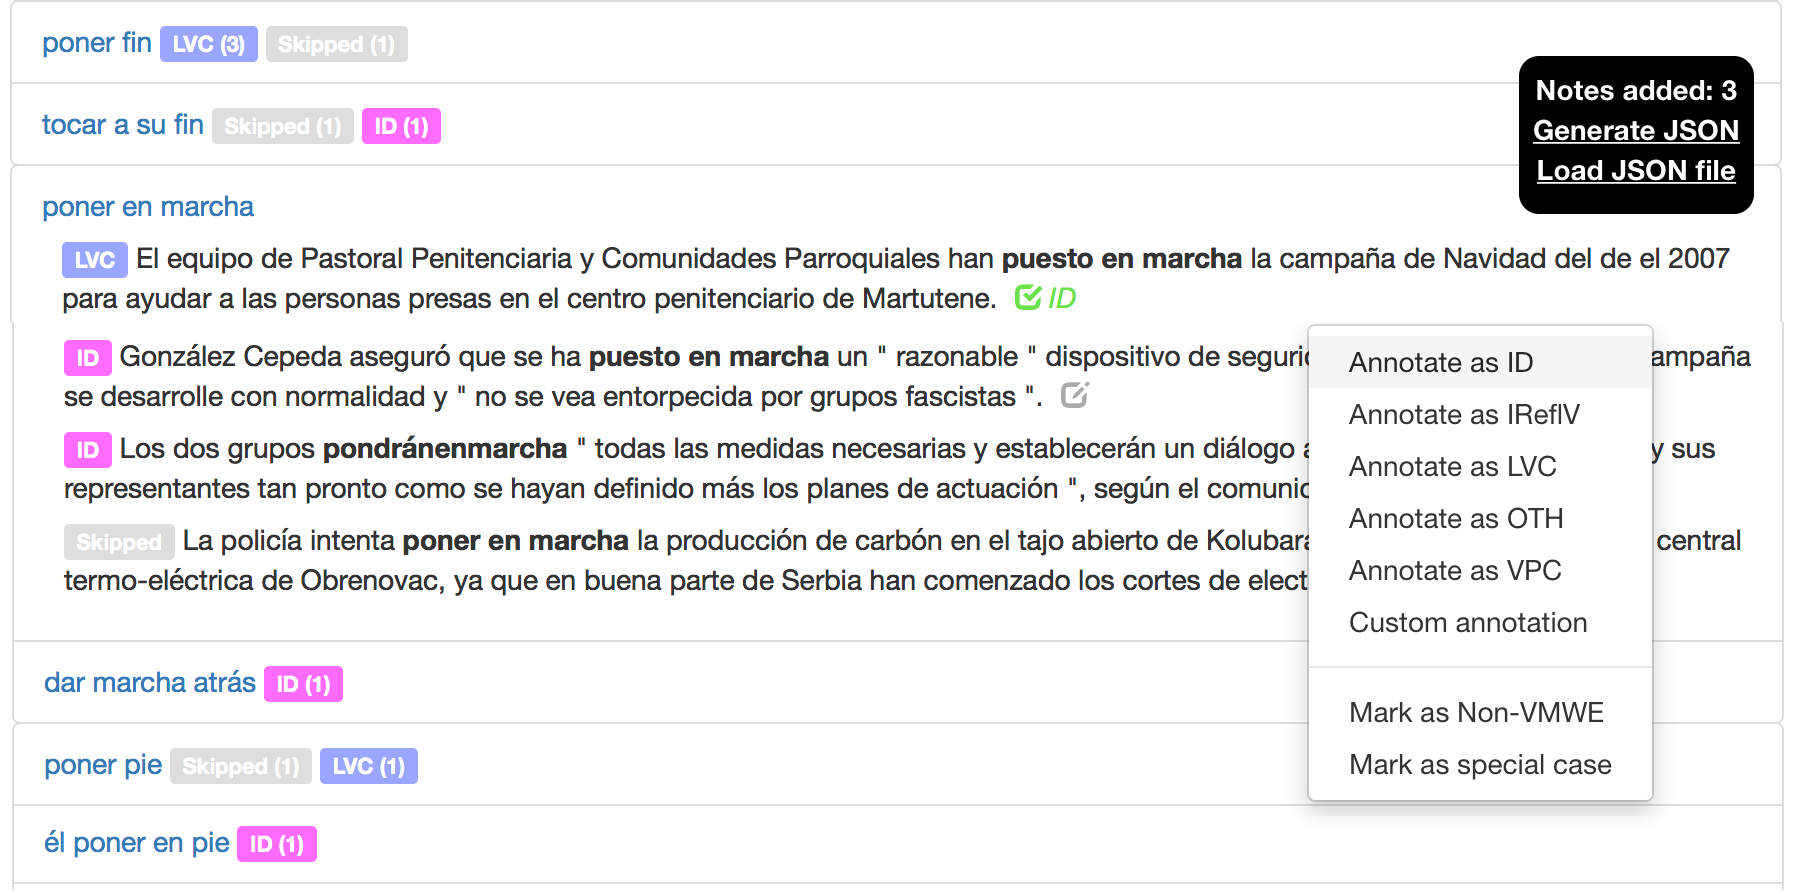
\includegraphics[width=0.95\textwidth]{figures/Validation_ES_bis.png}%{Validation_ES_small.png}
\caption{
Consistency-check tool at work. Here, (ES) \exlitidio{\lex{poner en marcha}}{to put in march}{to start} was annotated once as LVC, twice as ID and once skipped. The clickable icon next to each example allows the user to add, correct or delete an annotation. VMWEs with the same noun, e.g. (ES) \exlitidio{\lex{poner fin}}{to put end}{to terminate} and \exlitidio{\lex{tocar a su fin}}{to touch to its end}{to come to its end} on the top of the screen, are gathered so as to enhance annotation consistency, especially for LVCs.
%(here: \exidio{fin}{end}, \exidio{marcha}{march} and \exidio{pie}{foot}) are gathered so as to enhance annotation consistency, especially in LVCs.
%Validation tool at work. Here, the LVC (ES) \textit{celebrar reunión} 'to hold a meeting' was annotated by one annotator and wrongly skipped by two others. The clickable icon next to each example allows the user to add, correct or delete an annotation.
% in 3 other occasions. 
%Thanks to the validation tool, cases like this one were spotted and annotations were added, deleted or corrected as needed be.
}
\label{fig:validationES}
\end{figure}

%%%%%%%%%%%%%%%%%%%%%%%%%%%%%%%%%%%%%%%%%%%%%%%%%%%%%%%%%%%%%%%%%%%%%%%%%%%%%%%%%%%%%%%%%%%%%%%%%%%%%%%%%%%%%%%%%%%%%%%%%%%%%%%%%%%%%%%%%%%%%%%%%%%%%%%%%%%%%%%%%%%%%%%%%%%%%%%%%%%%%%%%%%%%%%%%%%%%%%%%%%%%
%%%%%%%%%%%%%%%%%%%%%%%%%%%%%%%%%%%%%%%%%%%%%%%%%%%%%%%%%%%%%%%%%%%%%%%%%%%%%%%%%%%%%%%%%%%%%%%%%%%%%%%%%%%%%%%%%%%%%%%%%%%%%%%%%%%%%%%%%%%%%%%%%%%%%%%%%%%%%%%%%%%%%%%%%%%%%%%%%%%%%%%%%%%%%%%%%%%%%%%%%%%%
\section{Properties of the annotated corpus}
\label{sec:corpora}
%\input{chapters/15.corpora}
\tabref{tab:corpora-overview} provides overall statistics of the corpus annotated for the shared task.\footnote{
The split into training and test corpora is indicated in \citet{MWEWorkshop}.} In total, it contains almost 5,5 million tokens, 274 thousand sentences and 62 thousand VMWE annotations. 
%In total, the corpora contain 230,062 sentences for training and 44,314 sentences for testing. These correspond to 4,5M and 900K tokens, with 52,724 and 9,494 annotated VMWEs, respectively. 
The amount and distribution of VMWEs over categories varies considerably across languages.

\begin{table}[t]
\centering
\setlength{\tabcolsep}{0.9mm}

\begin{tabularx}{.95\textwidth}{lrrrrrrrr}
\lsptoprule
\multirow{2}{*}{Language} & \multirow{2}{*}{Sentences} & \multirow{2}{*}{Tokens} & \multicolumn{6}{c}{VMWE occurrences} \\\cmidrule{4-9}
& & & All & IDs & IReflVs & LVCs & OTHs & VPCs \\
\midrule
BG & 8,860 & 200,128 & 2,406 & 517 & 1,376 & 511 & 2 & 0 \\
CS & 49,431 & 833,193 & 14,536 & 1,611 & 10,000 & 2,923 & 2 & 0 \\
DE & 7,500 & 144,856 & 2,947 & 1,219 & 131 & 218 & 10 & 1,369 \\
EL & 8,811 & 226,265 & 2,018 & 642 & 0 & 1,291 & 37 & 48 \\
ES & 4,634 & 159,807 & 1,248 & 362 & 556 & 320 & 10 & 0 \\
FA & 3,226 & 55,207 & 3,207 & 0 & 0 & 0 & 3,207 & 0 \\
FR & 19,547 & 486,005 & 4,962 & 1,905 & 1,418 & 1,633 & 6 & 0 \\
HE & 7,000 & 147,361 & 1,782 & 116 & 0 & 380 & 693 & 593 \\
HU & 4,311 & 108,175 & 3,499 & 0 & 0 & 730 & 0 & 2,769 \\
IT & 17,000 & 427,848 & 2,454 & 1,163 & 730 & 482  & 6 & 73 \\
LT & 14,863 & 256,235 & 502 & 287 & 0 & 215 & 0 & 0 \\
MT & 10,600 & 152,285 & 1,272 & 446 & 0 & 693 & 133 & 0 \\
PL & 13,606 & 220,934 & 3,649 & 383 & 1,813 & 1,453 & 0 & 0 \\
PT & 22,240 & 414,020 & 3,947 & 910 & 596 & 2,439  & 2 & 0 \\
RO & 51,500 & 879,427 & 4,540 & 599 & 2,786 & 1,154 & 1 & 0 \\
SL & 11,411 & 235,864 & 2,287 & 375 & 1,198 & 231 & 4 & 479 \\
SV & 1,800 & 29,517 & 292 & 60 & 17 & 27 & 2 & 186 \\
TR & 18,036 & 362,077 & 6,670 & 3,160 & 0 & 2,823 & 687 & 0 \\
\midrule
Total & 274,376 & 5,439,204 & 62,218 & 13,755 & 20,621 & 17,523 & 4,802 & 5,517 \\
\lspbottomrule       
\end{tabularx}
\caption{Overview of the annotated corpora in terms of the number of sentences, of tokens (whether belonging to the annotated VMWEs or not), and of the annotated VMWEs occurrences (overall and per category).}\label{tab:corpora-overview}
\end{table}
%\eb{question: Should be really table captions above and figure captions below?}\as{I think this is the LangSci style.}

No category was used in all languages, but the two universal categories, ID and LVC, were used in almost all languages. In Hungarian, no ID was annotated due to the genre of the corpus, mainly composed of legal texts. In Farsi, no categorisation was performed (\sectref{sec:lang-spec-guide}), and all annotated VMWEs are marked as OTH instead.
%therefore, the OTH category has special semantics there: it does not mean that a VMWE cannot be categorized because of its linguistic characteristics, but rather that the categorization tests were not applied. 

The most frequent category is IReflV, in spite of it being quasi-universal, mainly due to its prevalence in Czech. IReflVs were annotated in all Romance and Slavic languages, and in German and Swedish\il{Swedish}. VPCs were annotated in German, Swe\-dish, Greek, Hungarian, Hebrew, Italian, and Slovene. In the three last languages this category had a language-specific interpretation, as was the case of OTH in Hebrew and Turkish  (\sectref{sec:lang-spec-guide}). No language-specific categories have been defined. 
%However, the high frequency of OTH in some languages is a hint that they might be necessary, especially for
%non-Indo-European languages like HE, MT and TR.%Interestingly, these languages are also morphologically rich.
%{\bf ADDED MC 5 feb}: 

All the corpora are freely available on the LINDAT/CLARIN platform.\footnote{\url{http://hdl.handle.net/11372/LRT-2282}} The VMWE annotations are released under Creative Commons licenses, with constraints on commercial use and sharing for some languages. Some languages use data from other corpora (notably from the UD project), including additional annotations. These are released under the terms of the original licenses.

%%%%%%%%%%%%%%%%%%%%%%%%%%%%%%%%%%%%%%%%%%%%%%%%%%%%%%
\subsection{Format}
\label{sec:format}
%\input{chapters/15.format}

The official format of the annotated data is the parseme-tsv format\is{parseme-tsv},\footnote{\url{http://typo.uni-konstanz.de/parseme/index.php/2-general/184-parseme-shared-task-format-of-the-final-annotation}} exemplified in \figref{fig:format}. It is adapted from the CoNLL format, with one token per line and an empty line indicating the end of a sentence. Each token is represented by 4 tab-separated columns featuring (i) the position of the token in the sentence, or a range of positions (e.g.\ \texttt{1--2}) in case of MWTs such as contractions; (ii) the token surface form; (iii) an optional \texttt{nsp} (no space) flag indicating that the current token is adjacent to the next one; %(without any space character), 
and (iv) an optional VMWE code composed of the VMWE's consecutive number in the sentence and -- for the initial token in a VMWE -- its category, for example, \texttt{2:ID} if a token is the first one in  an idiom which is the second VMWE in the current sentence. In case of nested, coordinated or overlapping VMWEs, multiple codes are separated with a semicolon.

%This format has been used by the language leaders (prior to the annotation stage) to compile the corpus specific to their language. This step 
Formatting of the final corpus required a language-specific tokenisation procedure, which can be particularly tedious in languages presenting contractions. For instance, %where there are multiple tokens within the same word, 
%e.g., (FR) 
(FR) \exlit{du}{of-the} is a contraction of the preposition (FR) \exlit{de}{of} and the article (FR) \exlit{le}{the.\textsc{masc}}. 

%Moreover, (for most languages?) the parseme-tsv files were also accompanied with other layers of linguistic analysis, namely POS and dependecy tags . These were either already existing or newly acquired for the purposes of the current task and were also made available to the participating systems.
Some language teams resorted to previously annotated corpora %in CoNLL-U format
which have been converted to the parseme-tsv format automatically (or semi-automatically if some tokenisation rules were revisited). 
%On the contrary, other languages used already existing tools for tokenisation, POS and dependency parsing on corpora that were compiled especially for the specific task.
%Finally, with the help of the FLAT developing team, we have set up a script to convert the parseme-tsv format into the FoLIA format (used by the FLAT web-application), and a reversed script to do the opposite conversion after all the annotations have been collected.
Finally, scripts for converting the parseme-tsv format into the FoLiA format and back were developed to ensure corpus compatibility with FLAT (\ref{sec:flat}).

%\capa{This can be linked to the FLAT section where Martin explains how a converter was added to the platform?}

%MOVED TO THE ST CHAPTER
%Note that tokenisation is closely related to MWE identification, and it has been shown that performing both tasks jointly may enhance the quality of their results \citep{nasr:acl:2015}. However, the data we provided consist of pre-tokenised sentences. This implies that we expect typical systems to perform tokenisation prior to VMWE identification, and that we do not allow the tokenisation output to be modified with respect to the ground truth. The latter is necessary since the evaluation measures are token-based (cf. Chap.~SVARAY-ET-ALL-ST, Sec.~MEASURES). This approach may disadvantage systems which expect untokenised raw text on input, and apply their own tokenisation methods, whether jointly with VMWE identification or not. We are aware of this bias, and we did encourage such systems to participate in the shared task, provided that they define re-tokenisation methods so as to adapt their outputs to the tokenisation imposed by us.


%\begin{figure}[ht]
%\centering
%\begin{small}
%\setlength{\tabcolsep}{1mm}
%\begin{tabular}{rlll|rlll}
%1-2 & Wouldn't & & & 
%~~~1 & They & & \\

%1   & Would & & & 
%~~~2   & were & & \\

%2   & not & & &
%~~~3   & \textbf{letting} & & 1:VPC;2:VPC \\

%3   & questioning & & &
%~~~4   & him & & \\     

%4   & colonial & & &
%~~~5   & \textbf{in}  & & 1 \\

%5   & boundaries & & & 
%~~~6   & and & &  \\ 

%6   & \textbf{open} & & 1:ID~~~ &  
%~~~7   & \textbf{out} & & 2 \\

%7   & a & & & 
%~~~8 & .  & nsp &  \\

%8   & dangerous & &  \\
%9   & \textbf{Pandora}  & nsp & 1 & & \\
%10  & \textbf{'}        & nsp & 1 & & \\
%11  & \textbf{s}        &     & 1 & & \\
%12  & \textbf{box}      & nsp & 1 & & \\
%13  & ? & & 

%\end{tabular}
%\end{small}
%\caption{Annotation of two sample sentences containing a contraction %(\textit{wouldn't}), a verbal idiom, and two overlapping VPCs.}
%A verbal idiom \textit{open a pandora's box} annotated in a sample sentence containing a MWT (\textit{wouldn't}) and a MTW (\textit{Pandora's}).} 
%\label{fig:format}
%\end{figure}

%\begin{wrapfigure}{L}{0.45\textwidth}
\begin{figure}[ht]
\centering
\begin{small}
\setlength{\tabcolsep}{5.5mm}
\begin{tabular}{rlll}
1-2 & Wouldn't & & \\
1   & Would & & \\
2   & not & & \\
3   & questioning & & \\     
4   & colonial & & \\
5   & boundaries & & \\ 
6   & open & & 1:ID \\
7   & a & & \\
8   & dangerous & &  \\
9   & Pandora  & nsp & 1 \\
10  & '        & nsp & 1 \\
11  & s        &     & 1 \\
12  & box      & nsp & 1  \\
13  & ? & &  \\
&&& \\
1 & They & & \\
2 & were & & \\
3   & letting & & 1:VPC;2:VPC \\
4   & him & & \\
5   & in  & & 1 \\
6   & and & &  \\
7   & out & & 2 \\
8   & .  & nsp &  \\
\end{tabular}
\end{small}
\caption{Annotation of two sample sentences containing a contraction (\textit{wouldn't}), a verbal idiom, and two overlapping VPCs.}
\label{fig:format}
%\end{wrapfigure}
\end{figure}

%%%%%%%%%%%%%%%%%%%%%%%%%%%%%%%%%%%%%%%%%%%%%%%%%%%%%%
\subsection{Inter-annotator agreement}
\label{sec:iaa}
%\input{chapters/15.iaa}

Inter-annotator agreement (IAA)\is{inter-annotator agreement} measures are meant to assess the hardness of the annotation task, as well as the quality of the annotation guidelines, of the annotation methodology, and of the resulting annotations. Defining such measures is not always straightforward due to the challenges listed in \sectref{sec:methodology}.

\largerpage
%In this respect, our annotation task is challenging since it enhances \citep{DBLP:journals/coling/MathetWM15}: (a) unitising (identifying boundaries of VMWEs in text), (b) categorization (assigning the identified VMWEs to one of the VMWE categories), (c) nesting, (d) free-overlap and (d) sporadicity (not all text tokens are subject to annotation). 
%Two processes are to be assessed: (a) unitising, i.e. identifying boundaries of VMWEs in text, and (b) categorization, i.e. assigning the identified VMWEs to one of the VMWE categories ($\S$~\ref{sec:methodology}).  To this aim, for some languages, a number of sentences were annotated by two annotators.  
%\cara{I added some details, OK?}
To assess unitising, two annotators double-annotated an extract of the corpus in each language. We then calculated the MWE-based F-score ($F1_{unit}$) of one annotator with respect to the other.\footnote{That is, we suppose that one annotator represents the system, and the other one represents the gold standard. Note that F-score is symmetrical (depending on the order, recall and precision are inverted), so none of the two annotators is prioritised.} MWE-based F-score is defined in \citet{MWEWorkshop} and was used to evaluate the systems submitted to the shared task.  %\as{It's the per-VME F-score. Shouldn't it be teh per-token F-score?} 

We also report an estimated Cohen's $\kappa$ ($\kappa_{unit}$).  %\as{A reference?}.  
Measuring IAA, particularly $\kappa$, for unitising is not straightforward due to the absence of negative examples, that is, spans for which both annotators agreed that they are not VMWEs. From an extreme perspective, any combination of a verb with other tokens (of any length) in a sentence is a potential VMWE.\footnote{Also note that annotated segments can  overlap.} Consequently, as the density of VMWEs in most languages is rather low, one can argue that the probability of chance agreement approaches 0, %(i.e., $p_e \to 0$) 
and IAA can be measured simply using the observed agreement $F1_{unit}$. However, in order to provide 
%a lower bound 
a possibly less biased measure to the reported F-scores, we assume that the total number of stimuli in the annotated corpora is 
approximately equivalent to the number of %\as{\sout{words of part-of-speech category}} 
verbs, which %\sout{and that can be conservatively} 
%can roughly be estimated by 
is slightly higher than the number of sentences. We roughly estimate this quantity as the number of sentences plus the number of VMWEs annotated by at least one annotator.\footnote{In other words, the number of items on which both annotators agree as being no VMWEs is estimated as the number of sentences. 
This assumption ignores the fact that some verbs may be part of more than one VMWE, since this is rare.} 
%Thus, to obtain $\kappa_{unit}$, we assume that the total number of items annotated equals the number of verbs, which in turn is estimated as the number of sentences plus the number of VMWEs annotated by at least one annotator.%\as{$\kappa_{\textit{cat}}$
%Isn't it rather  $\kappa_{seg}$?}
%$\kappa_{unit}$ is the IAA for unitising based on this assumption.
%
%sentences decreased by the number of VMWEs annotated by any of the two annotators.}
%To obtain $\kappa_{unit}$, we assume that the total number of items annotated equals the number of verbs, which in turn is estimated as the number of sentences plus the number of VMWEs annotated by at least one annotator.\footnote{In other words, we assume that the total number of items for which both annotators agree that they are not VMWEs equals the number of sentences. This assumption ignores the fact that some verbs may be part of more than one VMWE, since this is rare.}
%\cara{I find this explanation of $\kappa_{unit}$ insufficient to reproduce the results. We should give a more precise formula. I cannot find the equation or the program that calculates this in the ST repositories and archives.}
%\as{The way I understand it is that if we use notations from \url{https://en.wikipedia.org/wiki/Cohen's_kappa} then we have a problem with knowing cell $d$ of the matrix. The above estimation simply assumes that $d$ is equal to the number of sentences minus $a+b+c$. Is that right?}
%\as{I do not understand this: which can be interpreted as a more conservative performance measure for (a)}. 
Finally, to assess categorisation, we apply the standard $\kappa$ ($\kappa_{cat}$) to the VMWEs for which annotators agree on the span. 

Due to time and resource constraints, the majority of the corpus for most languages was annotated by a single annotator. % (and possibly homogenised, as explained in Sec.~\ref{sec:consistency}). 
Only small fractions were double-annotated for the purpose of the IAA calculation. 
All available IAA results are presented in \tabref{iaa-table}.
For some languages the IAA in unitising is rather low. We believe that this results from particular annotation conditions. In Spanish, the annotated corpus is small (\tabref{tab:corpora-overview}), %\eb{\ref{tab:corpora-overview}})
so the annotators did not become sufficiently accustomed to the task. A similar effect occurs in Polish and Farsi, where the first annotator performed the whole annotation of the train and test corpora, while the second annotator only worked on the IAA-dedicated corpus. The cases of Hebrew, and especially of Italian, should be studied more thoroughly in the future. Note also that in some languages the numbers from \tabref{iaa-table} are a lower bound for the quality of the final corpus, due to post-annotation homogenisation  (\sectref{sec:consistency}). 


\begin{table}
\centering
\begin{tabularx}{0.79\textwidth}{c@{\qquad}rrrrrll}
\lsptoprule
& \#S&\#T& \#A$_1$&\#A$_2$& F1$_{\textit{unit}}$ &$\kappa_{\textit{unit}}$&  $\kappa_{\textit{cat}}$\\\midrule
\textbf{BG}	&	608	&	27491	&	298	&	261	&	81.6	&	0.738	&	0.925	\\
\textbf{EL}	&	1383	&	33964	&	217	&	299	&	68.6	&	0.632	&	0.745	\\
\textbf{ES}	&	524	&	10059	&	54	&	61	&	38.3	&	0.319	&	0.672	\\
\textbf{FA}	&	200	&	5076	&	302	&	251	&	73.9	&	0.479	&	n/a	\\
\textbf{FR}	&	1000	&	24666	&	220	&	205	&	81.9	&	0.782	&	0.93	\\
\textbf{HE}	&	1000	&	20938	&	196	&	206	&	52.2	&	0.435	&	0.587	\\
\textbf{HU}	&	308	&	8359	&	229	&	248	&	89.9	&	0.827	&	1.0	\\
\textbf{IT}	&	2000	&	52639	&	336	&	316	&	41.7	&	0.331	&	0.78	\\
\textbf{PL}	&	1175	&	19533	&	336	&	220	&	52.9	&	0.434	&	0.939	\\
\textbf{PT}	&	2000	&	41636	&	411	&	448	&	77.1	&	0.724	&	0.964	\\
\textbf{RO}	&	2500	&	43728	&	183	&	243	&	70.9	&	0.685	&	0.592	\\
\textbf{TR}	&	6000	&	107734	&	3093	&	3241	&	71.1	&	0.578	&	0.871	\\
\lspbottomrule
\end{tabularx}
\caption{IAA scores: \#S, and \#T show the the number of sentences and tokens in the double-annotated sample used to measure IAA, respectively. \#A$_1$ and \#A$_2$ refer to the number of VMWE instances annotated by each of the annotators.  
%F$_{\textit{seg}}$  and $\kappa_{\textit{seg}}$ indicate IAAs by reporting F-score and Kappa only considering the span of VMWEs. For those VMWEs that are annotated by both annotators, $\kappa_{\textit{cat}}$ reports Kappa as a measure of agreement when assigning VMWEs to their respective categories.
}
\label{iaa-table}
\end{table}

%\todo{CR: I suggest removing \#A1 and \#A2, increase font and reduce caption, which is currently bigger than the table itself.}
%\as{I think that \#A_1 and \#A_2 are important to give an idea of the size of the sample (it is not very big).}

A novel proposal of the holistic $\gamma$ measure \citep{DBLP:journals/coling/MathetWM15}  combines unitising and categorisation agreement in one IAA score, because both annotation subtasks are interdependent. In our case, however, separate IAA measures seem preferable both due to the nature of VMWEs and to our annotation methodology. Firstly, VMWEs are known for their variable degree of non-compositionality. In other words, their idiomaticity is a matter of scale. But this fact is not accounted for in current corpus annotation standards and identification tools, which usually rely on binary decisions, i.e. a candidate is seen as a VMWE or a non-VMWE, with no gradation of this status. Such a binary model is largely sub-optimal for a large number of grey-zone VMWE candidates. 
% require the MWE-hood, conversely, to be a binary property, which sub-optimally models a large number of grey-zone VMWE candidates. 
However, once a VMWE has been considered valid,  its categorisation appears to be significantly simpler, as shown in the last 2 columns of \tabref{iaa-table} (except for Romanian and Hebrew). Secondly, as described in~\sectref{sec:identify}~\textendash~\sectref{sec:decision-tree}, our annotation guidelines are structured in two main decision trees~\textendash~an identification and a categorisation tree~\textendash~to be applied mostly sequentially. %\footnote{Identification hypotheses may be questioned in the categorization process in case of LVCs or IReflVs though.} 
Therefore, separate evaluation of these two stages may be helpful in enhancing the guidelines.


%%%%%%%%%%%%%%%%%%%%%%%%%%%%%%%%%%%%%%%%%%%%%%%%%%%%%%
\subsection{Cross-language analysis}
\label{sec:analysis}
%\input{chapters/15.analysis}

The common terminology and annotation methodology achieved in this endeavour enable cross-language observations. In this section we offer a comparative quantitative analysis of several phenomena relevant to the challenges   VMWEs pose in NLP, as discussed in \sectref{sec:sav:intro}. Namely, we analyse the lengths, discontinuities, coverage, overlapping and nesting of VMWEs across languages and VMWE types.

\begin{table}
\centering
\begin{footnotesize}
\setlength{\tabcolsep}{0.8mm}

\begin{tabularx}{0.99\textwidth}%{XXX}
%\begin{tabular}
{l@{\qquad}rrr@{\qquad}rr@{\qquad}rr@{\qquad}rrr@{\quad}rr}
%\begin{tabular}{l@{\qquad}rrr@{\qquad}rr@{\qquad}rr@{\qquad}rrr@{\qquad}rr}
\lsptoprule
 & \multicolumn{3}{c@{\qquad}}{Length of VMWE} & \multicolumn{9}{c}{Length of discontinuities (excl. VMWEs of length 1)} \\
% \midrule
%& & Mean & & & Mean & & & & & & & \\
% & & Abs &  & & Abs &  & \% &  &  &  & & \% \\
Lang. & Avg & MAD & =1 & Avg & MAD & 0 & \%0 & 1 & 2 & 3 & >3 & \%>3 \\
\midrule
BG & 2.45 & 0.63 & 1 & 0.64 & 1.05 & 1586 & 82.1 & 206 & 33 & 25 & 82 & (4.2\%) \\
CS & 2.30 & 0.46 & 0 & 1.35 & 1.53 & 6625 & 51.5 & 2357 & 1465 & 944 & 1461 & (11.4\%) \\
% MC debug of script 24/8/2017 ...
%DE & 2.85 & 1.44 & 715 & 2.96 & 2.94 & 619 & 35.7 & 283 & 159 & 142 & 529 & (30.5\%) \\
DE & 2.02 & 0.61 & 715 & 2.96 & 2.94 & 619 & 35.7 & 283 & 159 & 142 & 529 & (30.5\%) \\
EL & 2.45 & 0.61 & 3 & 0.94 & 1.08 & 870 & 57.4 & 389 & 124 & 50 & 82 & (5.4\%) \\
ES & 2.24 & 0.39 & 0 & 0.47 & 0.66 & 523 & 69.9 & 162 & 33 & 14 & 16 & (2.1\%) \\
FA & 2.16 & 0.27 & 0 & 0.42 & 0.70 & 2243 & 82.9 & 202 & 103 & 60 & 99 & (3.7\%) \\
FR & 2.29 & 0.44 & 1 & 0.65 & 0.80 & 2761 & 61.9 & 1116 & 336 & 125 & 123 & (2.8\%) \\
HE & 2.71 & 0.75 & 0 & 0.47 & 0.74 & 1011 & 78.9 & 129 & 54 & 43 & 45 & (3.5\%) \\
% MC debug of script 24/8/2017 ...
%HU & 4.78 & 13.27 & 2205 & 1.01 & 1.29 & 506 & 63.7 & 178 & 34 & 15 & 61 & (7.7\%) \\
HU & 1.27 & 0.39 & 2205 & 1.01 & 1.29 & 506 & 63.7 & 178 & 34 & 15 & 61 & (7.7\%) \\
IT & 2.58 & 0.64 & 2 & 0.28 & 0.46 & 1580 & 80.9 & 278 & 56 & 22 & 16 & (0.8\%) \\
LT & 2.35 & 0.53 & 0 & 0.72 & 0.94 & 261 & 64.9 & 79 & 36 & 9 & 17 & (4.2\%) \\
MT & 2.64 & 0.68 & 7 & 0.34 & 0.53 & 589 & 77.0 & 123 & 33 & 12 & 8 & (1.0\%) \\
PL & 2.11 & 0.20 & 0 & 0.53 & 0.77 & 2307 & 73.3 & 470 & 195 & 90 & 87 & (2.8\%) \\
PT & 2.19 & 0.37 & 76 & 0.67 & 0.78 & 1964 & 58.3 & 1016 & 223 & 82 & 86 & (2.6\%) \\
RO & 2.15 & 0.25 & 1 & 0.55 & 0.72 & 2612 & 64.7 & 689 & 693 & 32 & 13 & (0.3\%) \\
SL & 2.27 & 0.43 & 14 & 1.47 & 1.54 & 787 & 44.4 & 445 & 221 & 118 & 202 & (11.4\%) \\
SV & 2.14 & 0.25 & 0 & 0.38 & 0.59 & 44 & 78.6 & 7 & 3 & 1 & 1 & (1.8\%) \\
TR & 2.06 & 0.11 & 3 & 0.57 & 0.57 & 3043 & 49.4 & 2900 & 162 & 33 & 28 & (0.5\%) \\
\lspbottomrule
\end{tabularx}
\end{footnotesize}
\caption{Length and discontinuities of VMWE occurrences in number of tokens in the training corpora. %VMWEs are counted in %tokens not types. 
%All occurrences rather than unique VMWEs are accounted for. 
Col.\ 2--3: average and mean absolute deviation (MAD) for length. Col.\ 4: number of single-token VMWEs. Col.\ 5--6: average and MAD for the length of discontinuities. Col.\ 7--8: number and percentage of continuous VMWEs. Col.\ 9--11: number of VMWEs with discontinuities of length 1, 2 and 3. Col.\ 12--13: number and percentage of VMWEs discontinuities of length $>3$.}\label{tab:corpora-train-characteristics}
\end{table}


\tabref{tab:corpora-train-characteristics} provides statistics about the length and discontinuities of annotated VMWEs in terms of the number of tokens.\footnote{Since the version published in \citet{MWEWorkshop}, we corrected a bug in the length average and MAD calculation, which impacted the results for languages containing VMWEs with one token only (especially DE and HU).} % appearing within the VMWE but not belonging to it). 
The average lengths range between 
%$2.1$ (in Polish) and $2.58$ (in Italian) tokens, 
$1.27$ (in Hungarian) and $2.71$ (in Hebrew) tokens, 
%\cara{Was outdated, please check -- old version said: ``$2.1$ (in Polish) and $2.58$ (in Italian) tokens''}
but the dispersion varies across languages: the mean absolute deviation (MAD) is $0.75$ for Hebrew, while it is $0.11$ for Turkish. Single-token VMWEs (length=1) are frequent in Hungarian and German ($63\%$ and $24\%$ %\cara{I get 715/2947=24\%, not 10\% as it was saying before} 
of all VMWEs, respectively) but rare or non-existent in other languages. %\as{Namely, $715$ ($10\%$) and $2205$ ($63\%$) VMWEs in DE and HU, respectively, are one-token occurrences, mainly separable VPCs, e.g. (DE) \exlitidio{\lex{auf}|\lex{machen}}{out|make}{open}, (HU) \exlitidio{\lex{át}|\lex{ruház}}{through dress}{to transfer}.} %\mc{TODO add example of why so many MWT in Hungarian}
%($715$ for DE more than $10\%$ of the occurrences, mainly  separable VPCs, e.g. \exlitidio{\lex{auf}|\lex{machen}}{out|make}{open}, and $2205$ for HU represent $63\%$ of the occurrences
The right part of \tabref{tab:corpora-train-characteristics} shows the lengths of discontinuities\is{verbal multiword expression!discontinuity} (gaps). This factor is measured in terms of the total number of tokens not belonging to a VMWE but appearing between its left- and  right-most lexicalised components. For instance, a gap of length 3 is counted in (DE) \exlitidio{jetzt \lex{bin} ich bestimmt \lex{aus} dem \lex{Alter heraus}}{now am I certainly out-of the age \textsc{part}}{now I am too old}. 
%(DE) \exlitidio{da \lex{fallen} wir immer \lex{durch} den \lex{Rost}}{then we always fall through the grate}{then we are always disadvantaged}. 
The discontinuities vary greatly across languages. While for Bulgarian, Farsi and Italian more than $80\%$ of VMWEs are continuous, only $35.7\%$ of German VMWEs do not have any gaps, and $30.5\%$ of them contain discontinuities of 4 or more tokens.

%%%%%%%%%%%%%%% Lengths broken down by category %%%%%%%%%%%%%
\begin{figure}
\centering
%\vspace{-10pt}
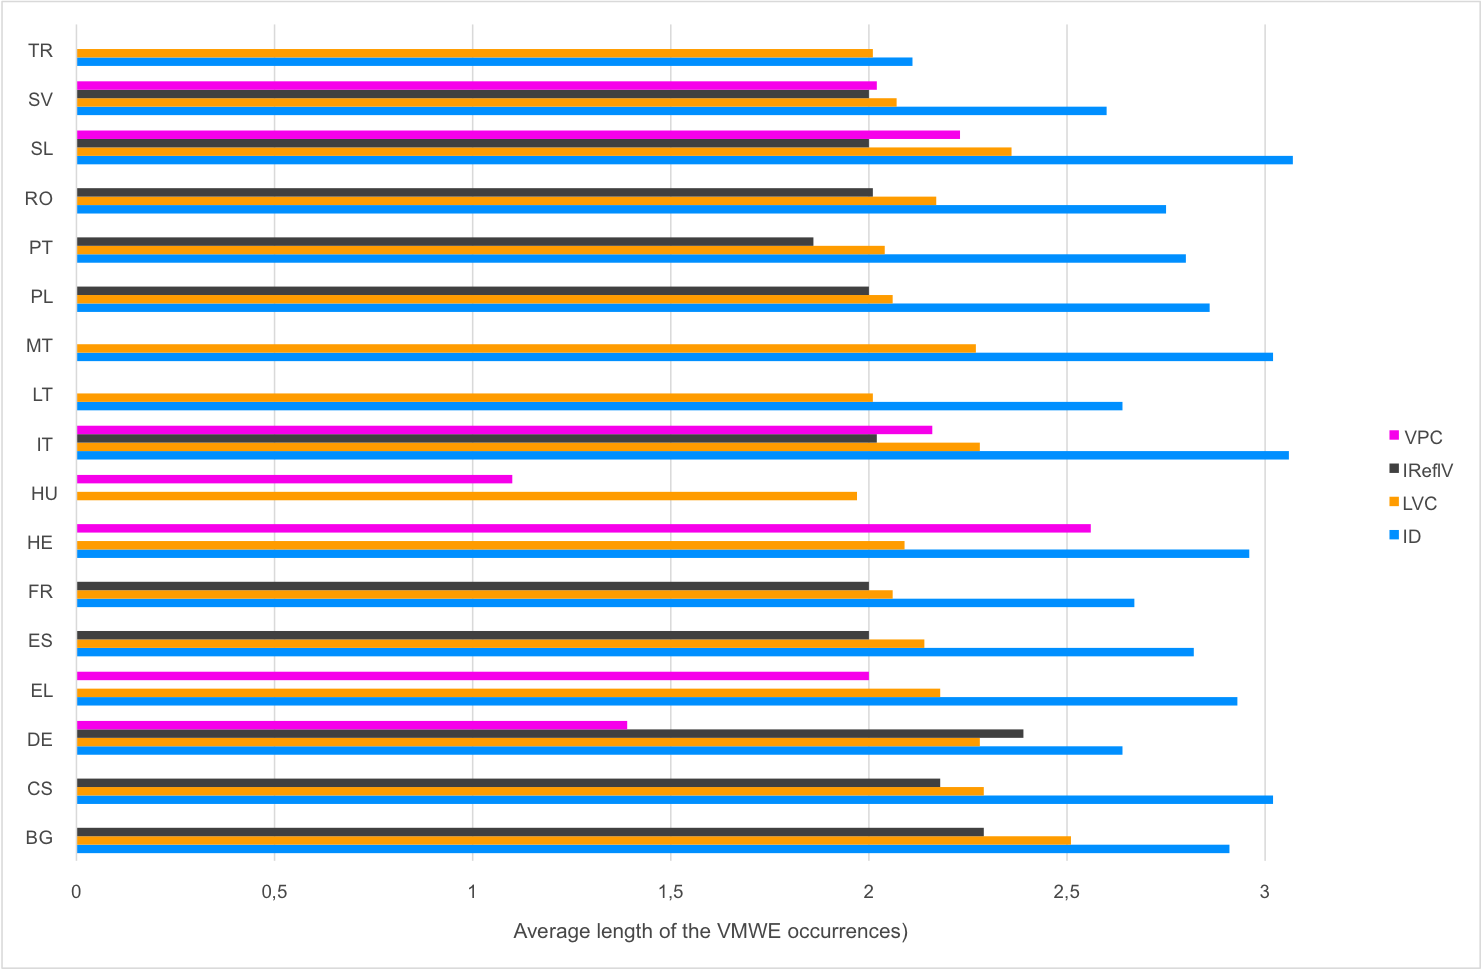
\includegraphics[width=1.0\textwidth]{figures/parseme-st-2017-BOOK-CORPUS-chart-length.png}
\caption{Average lengths of VMWE occurrences %broken down by VMWE 
per category, %counted 
in number of %token 
components. 
%VMWEs are counted in tokens not types, 
%The statistics are token-based 
%All occurrences rather than unique VMWEs are accounted for. 
Single-token VMWEs (frequent for Hungarian and German) are included.} %in the count .}
\label{fig:lengths-per-category}
\end{figure}
%%%%%%%%%%%%%%%%%%%%%%%%%%%%%%%%%%%%%%%%%%%%%%%%%%%%%%%%%%%%%
%The figures provided in Table~\ref{tab:corpora-train-characteristics} mask great differences between VMWE categories. We provide the lengths and discontinuity sizes broken down by category in 

\figref{fig:lengths-per-category} and \figref{fig:gaps-per-category} show a breakdown of the length and discontinuity scores per VMWE category (Farsi, where categorisation was not performed, is not included). Not surprisingly, %it can be seen that 
IDs are longer on average than all other categories (OTHs are omitted due to their rarity), and the average ID length ranges roughly between $2.5$ and $3$ components. The average lengths for the other categories are closer to $2$, which is expected given their definitions. Note though that VPCs are more contrasted across languages, with a low average length for German and Hungarian, due to the massive presence of single-token VMWEs. As far as IReflVs are concerned, a similar effect can be observed for some languages depending on morphological and tokenisation rules, due to the presence of IReflVs of length 1, for instance (ES) \exlitidio{\lex{referir}.\lex{se}}{to refer.\textsc{refl}}{to refer}. IReflVs of length greater than 2 in Czech, Bulgarian and German result from language-specific interpretations of the guidelines (\sectref{sec:lang-spec-guide}).

%\as{Looking at Fig.~\ref{fig:lengths-per-category} I wonder how an IReflV can have length greater than 2 in DE, CS and BG. Any idea?}

%%%%%%%%%%%%%%% Discontinuities broken down by category %%%%%
\begin{figure}
\centering
%\vspace{-10pt}
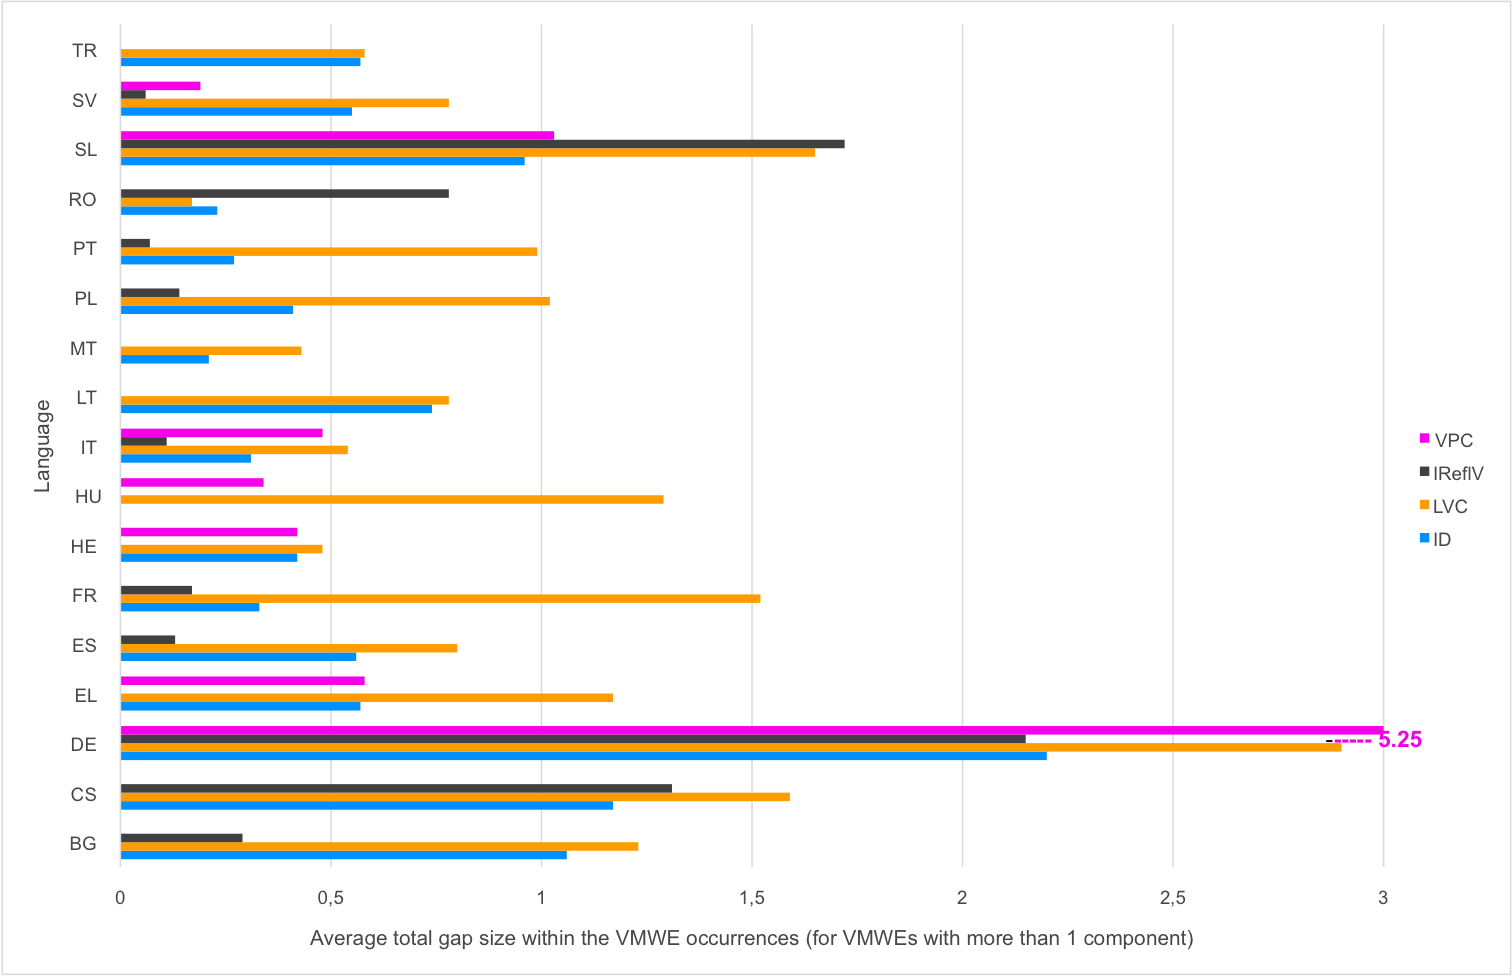
\includegraphics[width=1.0\textwidth]{figures/parseme-st-2017-BOOK-CORPUS-chart-discont.png}
\caption{Size of discontinuities in VMWEs. The gap size is the total number of tokens not belonging to a VMWE but appearing between its left- and  right-most lexicalised components.
%for a VMWE is the total number of tokens not belonging to it but appearing between two components of the VMWE. 
VMWEs of length 1 are not considered. For German the VPC average gap size is $5.25$.}
\label{fig:gaps-per-category}
\end{figure}
%%%%%%%%%%%%%%%%%%%%%%%%%%%%%%%%%%%%%%%%%%%%%%%%%%%%%%%%%%%%%
When comparing the lengths of discontinuities across languages (\figref{fig:gaps-per-category}), German stands clearly out %as having the high sizes for 
in all categories %, for obvious word order characteristics, 
and so does Slovene to a smaller extent (probably due to the language-specific interpretation of the VPC category, \sectref{sec:lang-spec-guide}), whereas Italian, Hebrew or Maltese show very few discontinuities. Note the difference for LVCs within Romance languages, which should be studied in more detail. %, to check consistence across languages. 
%When comparing categories, it can be seen that 
LVCs are clearly the category showing the longest discontinuities overall, mainly due to the presence of non-lexicalised determiners and pre-modifiers of the predicative nouns, although extraction of the nouns also comes into play.

%\capa{For part of this analysis we may want to cite another paper I know is being submitted to the special issue that precisely analyses the new/unseen VMWEs etc. instead of doing the same here.}\as{Yes, I'm also aware of this chapter. I'm sure we'll make cross-references at the end, when the volume is close to publication.}

While regularities do exist in the formation of MWEs, it essentially remains an idiosyncratic and lexical phenomenon. Hence, it is very likely that the annotated datasets cover only a small fraction of all the VMWEs %lexicons%, whether intra- or inter-domain, 
existing in each of the 18 languages. 
%, whether intra-domain or inter-domain, i.e. whether considering texts from the same domain as that annotated, or from different domains. 
In order to evaluate this coverage, we propose to measure the ratio of unknown VMWEs considering a corpus split into training and test sets, similar to the split used in the shared task \citep{MWEWorkshop}. In other words, we arbitrarily split the corpus into a training and a test set, and study 
%Stella's comment: studied (but we mean resent tense since we repeat this study with several splits)
 the proportion of VMWEs present in the test but absent in the training set.\footnote{See also \citetv{Maldonadotv} and \citetv{Taslimipoortv} for in-depth considerations on how the training vs. test corpus split influences the results of automatic VMWE identification.}
%\cara{Was: present in the train but absent in the test set - I inverted it, OK?} 

Ideally, we should perform this estimation on an intra- and inter-domain basis. 
%An ideal situation would be to evaluate on a set corresponding to a new text, whether of the same domain or of a different domain. 
Unfortunately, we do not know the domain of the source text for each annotated sentence.\footnote{For instance the French dataset contains the UD corpus, whose sentences come from various untraced sources and are mixed.} To circumvent this limitation, we can still provide a lower bound of the unknown VMWE ratios by considering different splits that use continuous portions of the corpus, as shown in \figref{fig:unknown-ratios}. For each language for which the morphological companion files were provided,
%with accompanying morphological information, 
we show the average rate of unknown % (multi-word tokens).} 
VMWEs\footnote{Matching of VMWEs in train and test sets is performed on lemmatised forms, and with limited normalisation of the order of components (in particular verb-noun for LVCs, and clitic-verb for IReflVs). Note that better normalisation should be performed in order to match multitoken VMWEs against their single-token variants.} computed over 5 cross-validation splits, plotted against the total number of VMWE occurrences. For instance for Italian we get an average unknown rate of $66.2\%$, with roughly $2{,}000$ annotated VMWE tokens, which means that, on average, in a fraction of $400$ VMWEs, two thirds are not present in the remaining $1{,}600$ VMWEs. %It can be seen that 
The ratios are rather high, except for Hungarian and Romanian. Although we would expect these scores to have negative correlation with the size of the annotated data, the plot shows great differences even among languages with comparable numbers of annotated VMWEs. We can hypothesise that other factors come into play, such as cross-language variability of domains, text genres and annotation quality.  
%besides the data size, other factors impact the ratios of unknown VMWEs, like 
%variable homogeneity within each corpus in terms of domain and genre, or differences in annotation quality.

%\begin{wrapfigure}{R}{0.5\textwidth}
\begin{figure}
\centering
%\vspace{-10pt}
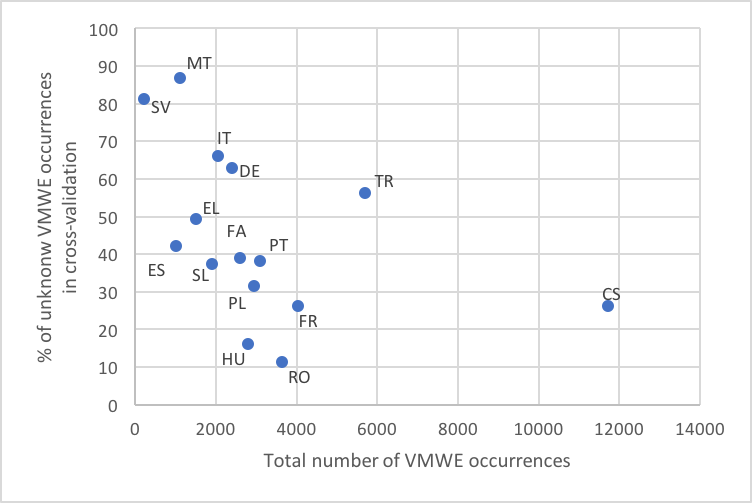
\includegraphics[width=0.8\textwidth]{figures/parseme-st-2017-BOOK-CORPUS-chart-ratio-unk-all.png}
\caption{Ratios of unknown VMWEs in the different language datasets. X-axis: the total number of VMWEs tokens in the train+test corpus. Y-axis: average proportion of unknown VMWEs (present in the test but not in the train set) when performing %5-fold 
cross-validation with 5 different train/test splits.}
\label{fig:unknown-ratios}
\end{figure}
%\end{wrapfigure} 

%We also investigated the frequency of overlapping and nested VMWEs  in the data.
%In the case of overlapping MWEs, one or more tokens of an MWE also form part of another MWE in the sentence. 
%For instance, the Portuguese sentence \textit{Ela est\'a com febre, dores no corpo e coriza} ``She has fever, her body aches and her nose is running'' contains three VMWEs (\textit{est\'a com febre}, \textit{est\'a com dores} and \textit{est\'a com coriza}). 
We also investigated two other challenging phenomena: overlapping\is{verbal multiword expression!overlapping} and nesting\is{verbal multiword expression!nesting} of VMWEs. The former was measured in terms of the frequency of tokens belonging to at least 2 VMWEs. It occurs -- most often due to ellipsis in coordinated VMWEs -- in most of the languages but rarely concerns more than two VMWEs at a time, as shown in \tabref{overlap}. 
%and they are most common in elliptic constructions: e.g.~in the Portuguese example, the verb and the preposition are ellipted from the second and third VMWEs. 
%Tokens that belong to more than two VMWEs at the same time can rarely be found in the corpora. 
The highest number of overlapping VMWEs was five, as seen in (\ref{pl:wykonywac-manewry}), where the light verb (PL) \exlit{wykonywać}{perform} is shared by five LVCs.
%: (PL) \exidio{Piloci \lex{wykonywali} podstawowe \lex{manewry} i serie \lex{wznosze\'n}, \lex{nurkowa\'n}, \lex{p\c{e}tli} i \lex{zwrot\'ow}}{The pilots performed basic maneuvers and series of climbs, dives, rolls and turns}. 

\ea \label{pl:wykonywac-manewry}
\settowidth \jamwidth{(PL)} 
\gll Piloci \lex{wykonywali} podstawowe \lex{manewry} i serie \lex{wznosze\'n}, \lex{nurkowa\'n}, \lex{p\c{e}tli} i \lex{zwrot\'ow}. \\
pilots performed basic maneuvers and series climbs.\textsc{gen}, dives.\textsc{gen}, rolls.\textsc{gen} and turns.\textsc{gen}\\ \jambox{(PL)}
\glt \idio{The pilots performed basic maneuvers and series of climbs, dives, rolls and turns.}
\z

%VMWEs a single token belongs to is five and can be found in the Polish data (\textit{Piloci wykonywali podstawowe manewry i serie wznosze\'n, nurkowa\'n, p\c{e}tli i zwrot\'ow} ``Pilots made basic maneuvers and series of ascents, dives, loops and turns''). \vv{Agata, can you please check this sentence?}
As far as nesting is concerned, measuring this phenomenon precisely, as defined in \sectref{sec:methodology}, would require the availability of syntactic annotations for all languages. Since this is not the case, we approximated nesting at the syntactic level by pairs of VMWEs $E_1$ and $E_2$ such that all lexicalised components of $E_2$ are placed between the left- and right-most lexicalised components of $E_1$. Single-token VMWEs were disregarded.
%only considered VMWEs with at least two tokens. %, thus single-token MWEs are not considered here. 
As the last line of \tabref{overlap} shows, such configurations occur very rarely in the data. 
%that the Czech data, which is the largest dataset, has the largest number of nested VMWEs, however, the general tendency shows that 
%nesting occurs very rarely in the data. 
%When they occur, they are usually due to relative clauses as in the French example \textit{Les trois arriv\'ees du Tour de France cycliste, qui se sont d\'eroul\'ees \ \`{a} Mende, se sont effectu\'ees sur l'a\'erodrome} ``The three arrivals of the Tour de France cyclist, which took place in Mende, happened in the aerodrome'' -- the two VMWEs here are \textit{arriv\'ees effectu\'ees} and \textit{se d\'eroul\'ees}. 
This might be due to the fact that large gaps introduced within the outer-most VMWEs by the nested structure are harder to process for the human mind.
 
\begin{table}[htp]
\setlength{\tabcolsep}{1pt}
%\begin{tabular}{l @{\qquad} l @{\qquad} l @{\qquad} ccccc @{\qquad} cc @{\qquad} ccccc @{\qquad} cccccc}
\begin{small}
\begin{tabularx}{\textwidth}{lcccccccccccccccccc}
%\begin{tabular}{lcccccccccccccccccc}
%\begin{tabular}{|l|l|ccccc|cc|ccccc|cccccc|}
\lsptoprule
  &  BG & CS & DE & EL & ES & FA & FR & HE & HU & IT & LT & MT & PL & PT & RO & SL & SV & TR \\\midrule
Overlap >= 2 & 0 & 520 & 122 & 5 & 22 & 1 & 60 & 235 & 30 & 73 & 0 & 1 & 44 & 65 & 53 & 0 & 1 & 19 \\
  & & {\scriptsize (1.6\%)} & {\scriptsize (2\%)} & &  & &  & {\scriptsize (5\%)} & & {\scriptsize (1.2\%)} &  &  & {\scriptsize (0.6\%)} & {\scriptsize (0.5\%)} & {\scriptsize (0.5\%)} &  &  &  \\
Overlap > 2 & 0 & 11 & 0 & 1 & 0 & 0 & 5 & 9 & 0 & 0 & 0 & 0 & 1 & 6 & 0 & 0 & 0 & 0 \\
Nested VMWEs & 4 & 29 & 1 & 0 & 0 & 0 & 1 & 0 & 1 & 3 & 0 & 0 & 4 & 1 & 0 & 2 & 0 & 0 \\
\lspbottomrule
\end{tabularx}
\end{small}
\caption{Overlapping and nested VMWEs. Overlap >=2 and >2: the token belongs to at least 2 or more than 2 VMWEs, respectively. Only percentages above 0.49\% are indicated. They are counted wrt. all tokens belonging to VMWEs.}
\label{overlap}
\end{table} 


%%%%%%%%%%%%%%%%%%%%%%%%%%%%%%%%%%%%%%%%%%%%%%%%%%%%%%%%%%%%%%%%%%%%%%%%%%%%%%%%%%%%%%%%%%%%%%%%%%%%%%%%%%%%%%%%%%%%%%%%%%%%%%%%%%%%%%%%%%%%%%%%%%%%%%%%%%%%%%%%%%%%%%%%%%%%%%%%%%%%%%%%%%%%%%%%%%%%%%%%%%%%
%%%%%%%%%%%%%%%%%%%%%%%%%%%%%%%%%%%%%%%%%%%%%%%%%%%%%%%%%%%%%%%%%%%%%%%%%%%%%%%%%%%%%%%%%%%%%%%%%%%%%%%%%%%%%%%%%%%%%%%%%%%%%%%%%%%%%%%%%%%%%%%%%%%%%%%%%%%%%%%%%%%%%%%%%%%%%%%%%%%%%%%%%%%%%%%%%%%%%%%%%%%%
\section{Language-specific studies based on the corpus}
\label{sec:corpus-studies}
%\input{chapters/15.corpus-studies}
Since its publication in January 2017, the PARSEME VMWE-annotated corpus has enabled studies in corpus linguistics in several languages. 

The French\il{French} corpus was addressed by \citet{Pasquer17}, who focuses on the variability\is{idiomatic variation} of the most frequent VMWEs. Three aspects are studied: (i) morphological variability of VMWE components, (ii) length and nature of discontinuities between the VMWE components, (iii) syntactic dependencies between the VMWE components and their dependents/governors. The results show a distinctly higher variability in LVCs than in IDs. Namely, nouns inflect and govern external modifiers, respectively, 8 and 1.7 times more often in LVCs (\exidio{il \lex{rend} les derniers \lex{hommages}}{he pays the last tributes}) than in IDs. IDs include a lexicalised determiner (\exidio{elle \lex{tourne la page}}{she turns the page} vs. \exidio{elle \lex{joue} un \lex{role}}{she plays a role}) and a compulsory negation (\exlitidio{ça \lex{ne paye pas de mine}}{it does not pay a face}{it is not much to look at}), 20 and 10 times more often than LVC, respectively.
LVCs exhibit discontinuities and passivise 1.5 and 29 times more often than IDs, respectively. 
Additionally, types of syntactic variants are listed and quantified for the 3 most variable VMWEs.  Interesting types of morphological variants, such as prefixations (\exlitidio{\lex{redonner raison}}{to re-give reason}{to admit again that someone is right}), are also revealed.

In Maltese\il{Maltese}, investigations on LVCs\is{light-verb construction} were also carried out in the PARSEME corpus extended with the Maltese UD corpus. The annotated LVCs were extracted and proofread, and the 20 most frequent light verbs (LVs) were listed. Those were used to find other candidate LVCs in a  larger raw corpus (not annotated for VMWEs). For each LV the number of unique predicative nouns they combine with could be established. The results show that some LVs are inherently light (e.g. \exidio{ta}{to give}, \exidio{ħa}{to take} and \exidio{għamel}{to make/do}) and combine with large numbers of nouns (here: 60, 48, and 46, respectively), while others are light only when combined with a few nouns (e.g. \exidio{ġarr}{to carry}, \exidio{laħaq}{to reach/achieve}, \exidio{talab}{to request/ask}). An analogous experiment, performed for nouns, shows that most of them occur with two LVs (\exidio{ta}{to give} and \exidio{ħa}{to take}), while only few (\exidio{appoġġ}{support}, \exidio{kura}{care/treatment} and \exidio{kenn}{shelter}) combine with many LVs. Other interesting findings are of etymological nature. Maltese is a language with influences from Semitic and Romance languages, as well as English. The inspected LVCs were mostly of Romance origin (70\%), some of Semitic (25\%) and some of English (5\%). Interestingly, some LVCs accommodate borrowings and Semitic elements that are no longer productive, for example, \exidio{\lex{ħa nifs}}{to take a breath} is ten times more frequent than the Semitic \exidio{niffes}{to breathe}. 

LVC-specific analyses were also performed in Lithuanian\il{Lithuanian}. Two groups of verbs were identified based on their frequencies in LVCs: 
(i) 4 high-connectivity verbs i.e. those that combine with large numbers of nouns:  \exlit{vykdyti}{to carry out} connects with 19 nouns, \exlit{atlikti}{to perform} -- 14, \exlit{turėti}{to have} -- 12, \exlit{daryti}{to do/to make} -- 10; 
(ii) 17 low-connectivity verbs i.e. those combining with less than 10 nouns, e.g. \exlit{teikti}{to deliver} -- 6, \exlit{surengti}{to arrange} -- 4, \exlit{imtis}{to undertake} -- 3, \exlit{priimti}{to accept} -- 3, \exlit{patirti}{to experience} -- 3,  \exlit{duoti}{to give} -- 3, \exlit{sudaryti}{to make} -- 3, etc. 
The numbers of the LVCs containing the verbs from (i) and (ii) are comparable -- 55 and 38, respectively -- but the diversity of the verbs is significantly higher in (ii) than in (i). 
The LVCs containing the verbs from group (i) seem to be the most prototypical ones, e.g. \exlit{\lex{vykdyti patikrinimus}}{to carry out inspections}, \exlit{\lex{atlikti analizę}}{to perform an analysis}, \exlit{\lex{daryti spaudimą}}{to put pressure}, etc. These findings pave the way towards developing a comprehensive list of light verbs for Lithuanian.

%%%%%%%%%%%%%%%%%%%%%%%%%%%%%%%%%%%%%%%%%%%%%%%%%%%%%%%%%%%%%%%%%%%%%%%%%%%%%%%%%%%%%%%%%%%%%%%%%%%%%%%%%%%%%%%%%%%%%%%%%%%%%%%%%%%%%%%%%%%%%%%%%%%%%%%%%%%%%%%%%%%%%%%%%%%%%%%%%%%%%%%%%%%%%%%%%%%%%%%%%%%%
%%%%%%%%%%%%%%%%%%%%%%%%%%%%%%%%%%%%%%%%%%%%%%%%%%%%%%%%%%%%%%%%%%%%%%%%%%%%%%%%%%%%%%%%%%%%%%%%%%%%%%%%%%%%%%%%%%%%%%%%%%%%%%%%%%%%%%%%%%%%%%%%%%%%%%%%%%%%%%%%%%%%%%%%%%%%%%%%%%%%%%%%%%%%%%%%%%%%%%%%%%%%
%\section{Findings}
\section{Interesting problems}
\label{sec:findings}
%\input{chapters/15.findings}
The considerable collective PARSEME corpus effort led us to confront various phenomena across different language families, various linguistic traditions, and annotation practices. As a result, some interesting findings allow us to view the VMWE phenomenon more globally, which should enable further cross-language generalisations. 

Since semantic non-compositionality is the most pervasive property of MWEs, it should possibly be captured by generic definitions and tests in a multilingual endeavour like ours. However, semantic properties show up in different languages via different morphological, syntactic and semantic means. As a result, some semantic non-compositionality phenomena cross word boundaries in some languages, and are therefore relevant to MWEs, and others do not. This distinction can also vary from language to language for the same phenomenon.

For instance, particles in Germanic and Finno-Ugric VPCs, like (EN) \ile{to \lex{turn off}}, have similar roles as prefixes in Slavic verbs, like (PL) \exlit{wy.łączyć}{to \textsc{part}.connect} $\Rightarrow$\idio{to turn off}. The former are traditionally considered separate lexemes, and can therefore form VMWEs with their governing verbs. The latter, conversely, are considered inherent components of verbs, and therefore cannot trigger MWE-related considerations.

Similarly, aspect\is{grammatical aspect} can be realised by various lexical, morphological and syntactic means, and can therefore be seen as either a semantic or a morphological feature (or both). For instance, perfective or continuous aspect can be introduced by inflection and analytical tenses: (EN) \ile{is doing}, \ile{has done}. Starting, continuation, completion and perfective aspect can also be expressed by specific verbs modifying other verbs: (EN) \ile{to start/continue/stop/complete the action}. Finally, in Slavic languages each verbal lexeme (i.e. independently of its inflected form), has inherent aspect, either perfective or imperfective, and is marked as a morphological feature (recognisable either by a prefix or by an ending): (PL) 
\exlit{robić}{to do.\textsc{imperf}}  vs. \exlit{z.robić}{to \textsc{part}.do.\textsc{perf}};
\exlitidio{wy.łączać}{to \textsc{part}.connect.\textsc{imperf}}{to turn off} vs. \exlitidio{wy.łączyć}{to \textsc{part}.connect.\textsc{perf}}{to turn off}. 
Therefore, in Slavic languages the verb in an LVC necessarily adds aspect to the predicate, so its status in Test 11 (\sectref{sec:lvcs}) should be examined along slightly different lines than in Romance and Germanic languages. Additionally, if adding any aspectual semantics to the predicate should necessarily block the LVC classification in Test 11, then (EN) \ile{to \lex{take} a \lex{decision}} should be annotated as an LVC, while (EN) \ile{\lex{taking} a \lex{decision}} might not. These observations led us to revise the LVC tests for future editions of the guidelines.

Another finding concerns productivity. Some verbs admit arguments from large semantic classes, and, conversely, some nouns select various verbal operators. More precisely, we observed 
the hardness of delimiting productive from non-productive\is{productivity} cases in VMWE categories: (i) whose semantic non-com\-po\-si\-tio\-na\-li\-ty is weak, or (ii) whose components are not content words. The former mainly concerns LVCs. We found no effective and reproducible way to distinguish lexical selection from selection of large semantic classes. For instance, (EN) \ile{to deliver} is often used with the class of nouns expressing formal speech acts such as \ile{speech}, \ile{lecture}, \ile{verdict}, etc. However, we can also use the verb \ile{to give} instead of \ile{to deliver} with the same class of nouns, which likely shows a productive rather than a strict lexical selection. Problem (ii) concerns VPCs, IReflVs and prepositional verbs. Namely, as the semantics of particles is hard to establish, we could come up with only one VPC-related test (\sectref{sec:vpcs}), which should clearly evolve in future work. Also, the ambiguity of various uses of the reflexive clitic, and the resulting hardness of the IReflV annotation, was stressed by many language teams. Finally, the non-compositionality of prepositional verbs was so hard to establish in the pilot annotation that we abandoned them in the final annotation.

\largerpage
We also underestimated the importance of modelling not only the semantic non-compositionality of idioms but their conventionalisation as well. As a result, we currently have no efficient way to distinguish MWEs from metaphors\is{metaphor}. The resemblance is strong since many idioms are metaphors, e.g. (PT) \exlitidio{ele \lex{abre mão}}{he opens hand}{he gives up}, but non-idiomatic metaphors, created for the need of a particular text, do occur, e.g. (PL) \exidio{podpisanie tej umowy to stryczek założony na szyję Polski}{signing this treaty is  a noose put around Poland's neck}. The difference is hard to tackle, and especially to test, since it seems to lie precisely in the fact that MWEs are conventionalised while metaphors are not necessarily so. A partial solution to this problem may probably stem from statistical estimations, although the ``long tail'' of conventionalised and still infrequent MWEs may largely resemble non-conventionalised metaphors. We put forward the MWE vs. metaphor distinction as a future research issue.

%%%%%%%%%%%%%%%%%%%%%%%%%%%%%%%%%%%%%%%%%%%%%%%%%%%%%%%%%%%%%%%%%%%%%%%%%%%%%%%%%%%%%%%%%%%%%%%%%%%%%%%%%%%%%%%%%%%%%%%%%%%%%%%%%%%%%%%%%%%%%%%%%%%%%%%%%%%%%%%%%%%%%%%%%%%%%%%%%%%%%%%%%%%%%%%%%%%%%%%%%%%%
%%%%%%%%%%%%%%%%%%%%%%%%%%%%%%%%%%%%%%%%%%%%%%%%%%%%%%%%%%%%%%%%%%%%%%%%%%%%%%%%%%%%%%%%%%%%%%%%%%%%%%%%%%%%%%%%%%%%%%%%%%%%%%%%%%%%%%%%%%%%%%%%%%%%%%%%%%%%%%%%%%%%%%%%%%%%%%%%%%%%%%%%%%%%%%%%%%%%%%%%%%%%
\section{Related work}
\label{sec:related-work}
%\input{chapters/15.related-work}
In this section we contextualise our work with respect to existing MWE typologies, annotation methodologies and annotated corpora.
%\cara{I added an introduction sentence to avoid an empty section header}

\subsection{MWE typologies}
\label{sec:related-typologies}

\begin{sidewaystable}
\begin{scriptsize}
\setlength{\tabcolsep}{1mm}

\begin{tabularx}{\textwidth}{p{2cm}p{1.5cm}p{1.0cm}p{8.5cm}>{\raggedright}p{1.7cm}>{\raggedright\arraybackslash}p{2.5cm}}
\lsptoprule
\textbf{Reference} & \textbf{Language} &\textbf{Scope} & \textbf{Classes} & \textbf{\# classified expressions} & \textbf{Defining criteria} \\\midrule

\citet{Sag2002a} & EN & MWEs and collocations & I. Lexicalised: 1. Fixed (\ile{by and large}); 2. Semi-fixed: non-decomposable idioms (\exidio{shoot the breeze}{chat}), compound nominals (\ile{part of speech}), proper names (\ile{San Francisco 49ers}); 3. Syntactically-flexible: VPCs (\ile{break up}), decomposable idioms (\ile{spill the beans}), LVCs (\ile{make a decision}); II. Institutionalised (\ile{traffic lights}) & unknown & lexicalisation, morphological and syntactic flexibility, semantic decomposability \\\midrule

\citet{baldwin2010multiword} & EN & MWEs and collocations & I. Nominal (\ile{golf club}, \ile{connecting flight}); II. Verbal: 1. VPCs (\ile{take off}, \ile{cut short}, \ile{let go}); 2. Prepositional verbs (\ile{come accross}); 3. LVCs (\ile{take a walk}); 4. Verb-noun idioms (\ile{shoot the breeze}); III. Prepositional: 1. Determinerless prepositional phrases (\ile{on top}, \ile{by car}); 2. Complex prepositions (\ile{on top of}, \ile{in addition to}) & unknown & syntactic structure \\\midrule

\citet{Melcuk10} & FR & MWEs and collocations & I. Pragmatic (\ile{emphasis mine}); II. Semantic: 1. Semantically compositional: clichés (\ile{in other words}), collocations (\ile{busy as a bee}, \ile{award a prize}); 2. Semantically non-compositional: quasi-locutions ((FR) \exlitidio{donner le sein}{give the breast}{breastfeed}), 2. Semi-locutions ((FR) \exlitidio{fruits de mer}{sea fruit}{seafood}), 3. Complete locutions ((FR) \exlitidio{en tenue d’Adam et Eve}{in Adam’s and Eve’s dress}{naked}) & 
%thousands of compositional and hundreds of non-compositional MWEs 
4,400 collocations, 3,200 locutions \citep{Pause17}
& selection constraints, semantic non-compositionality  \\\midrule

\citet{schneider2014} & EN & all MWEs & I. Strong (\ile{close call}); II. Weak (\ile{narrow escape})  & 3,500 occurrences & strength of association between words\\\midrule

\citet{Sheinfux17} & HE & verbal idioms &  I. Transparent figurative (\exidio{saw logs}{snore}); II. Opaque figurative (\exidio{shoot the breeze}{chat}); III. Opaque non-figurative (\exidio{take
umbrage}{feel offended}) & 15 VMWEs, 400 occurrences & transparency, figuration\\\midrule

%\citep{Parra:forth} & ES & all MWEs & I. Morphosyntactic types: 1. Adjectival, 2. Adverbial, 3. Conjunctional, 4. Nominal, 5. Prepositional, 6. Verbal: LVCs (\ile{make a decision}), periphrastic constr. (\exidio{pudo comprar}{could have bought}), verbal phrases (\ile{take the bull by the horns}), verbs with governed PP (\exidio{referirse a}{to refer to}), sentential (\exidio{cuando el río
%suena, agua lleva}{when there is smoke, there is fire}); II. Flexibility types: 1. Fixed, 2. Semi-fixed, 3. Flexible & 338 types & morphosyntactic structure, morphological and syntactic flexibility\\\hline 

%\citep{Sailetetal} & EN,DE,EL,HE, MK,NO,PL,RO, SK (HR,CS, ES,FR,SL,LA, RU,SR) & MWEs and collocations & I. By syntactic structure: 1. Nominal; 2. Verbal: LVCs, PVCs, V NP PP, V and V, V like V etc.; 3. Prepositional; 4. Adjectival; 5. Clausal; 6. Other; II. By fixedness/flexibility of MWE parts; III. By idiomaticity (lexical, syntactic, semantic, pragmatic, statistical)

\citet{Laporte:forth} & FR & MWEs and collocations & I. Lexicalised: 1. MWEs without support verbs: verbal (\ile{take stock}), nominal (\ile{traffic lights}), adverbial (\ile{for instance}); 2. Support-verb constr.: a. Vsup is not copula (\ile{have an aim}, \ile{get loose}), b. Vsup in copula (\ile{be a genius}, \ile{be angry}, \ile{be on time}); II. Non-lexicalised (\ile{salt and pepper}) & dozens of thousands of (lexicalised) MWEs & lexicalisation, presence of a support verb\\\midrule

This chapter & BG,CS,DE,EL, ES,FA,FR,HE, HU,IT,LT,MT, PL,PT,RO,SL, SV,TR & verbal MWEs & I. Universal: LVCs (\ile{make a decision}), IDs (\ile{spill the beans}); II. Quasi-universal: IReflVs ((FR) \exlitidio{s'avérer}{\textsc{refl}'reveal}{prove (to be)}), VPCs (\ile{take off}); III. OTH (\ile{drink and drive}, \ile{to voice act}) & 62,000 occurrences & universalism, syntactic structure, lexical, syntactic and semantic idiosyncrasy\\\lspbottomrule
\end{tabularx}
\caption{Various MWE classifications compared.}
\label{tab:mwe-classifications}
\end{scriptsize}
\end{sidewaystable}
%\eb{table~\ref{tab:mwe-classifications} overflows into the page margins... but I would ignore that...}

In previous approaches to modelling MWEs, various classifications of MWEs\is{multiword expression!typology} were put forward. 
Here, we focus on several proposals, summarised in \tabref{tab:mwe-classifications}, which seem relevant to our work in that they: 
(i) have been particularly influential in the NLP community \citep{Sag2002a,baldwin2010multiword,Melcuk10}
(ii) were tested against a representative data set \citep{Melcuk10}, notably in corpus annotation \citep{schneider2014}, %(ii) were tested against a large number of languages (\citep{Saileretal}), 
(iii) use MWE flexibility, which is a pervasive feature of verbal MWEs, as a major classification criterion \citep{Sag2002a}, 
(iv) focus exclusively on verbal MWEs \citep{Sheinfux17}, 
(v) put a verbal component in the heart of the classification criterion \citep{Laporte:forth}.

%Tab.~\ref{tab:mwe-classifications} shows a comparative study of those proposals. 

\citet{Sag2002a} is a highly influential seminal work whose MWE classification implements the hypothesis put forward by \citet{nunberg-94} about the correlation between the semantic decomposability\is{verbal multiword expression!decomposability} of an idiom and its syntactic flexibility\is{idiomatic variation}. According to this theory, it is because \ile{pull} can be rephrased as \ile{use} and \ile{strings} as \ile{one's influence} that the idiom \ile{to \lex{pull strings}} admits variations like \ile{to \lex{pull} all the (political) \lex{strings}}, \ile{the \lex{strings} he \lex{pulled}}, etc. The hypothesis has been criticised, e.g. by \citet{Sheinfux17} and \citet{Laporte:forth}, notably by demonstrating non-decomposable MWEs which still exhibit flexibility. The \citet{Sag2002a} classification also calls for adjustments in inflectionally rich and free-word-order languages. Still, it remains widely used, notably due to its usefulness for NLP applications. Namely, MWE flexibility is a major obstacle in MWE identification since it prohibits seeing a MWE as a ``word with spaces'' and using sequence labelling approaches.

\citet{baldwin2010multiword} assume the flexibility-driven classification by \citet{Sag2002a} and they additionally introduce an orthogonal typology based on purely syntactic criteria, that is, on the syntactic structure of the MWE. There, verbal subcategories are both English-specific and non-exhaustive since verb-noun idioms are considered, but not, for example, verb-adjective ones.

The typology of \citet{Melcuk10} is based, conversely, on mainly semantic criteria. Different types of semantic compositionality are defined, and non-composi-tional\is{non-compositionality} subtypes are those where the semantic head is missing. The latter further subdivide into: (i) \emph{quasi-locutions} in which the meanings of the components are combined, as in (FR) \exlitidio{\lex{donner le sein}}{to give the breast}{to breastfeed}, (ii) \emph{semi-locutions} which include the meaning of only a part of their components, as in (FR) \exlitidio{fruits de mer}{sea fruit}{seafood}, (iii) \emph{complete locutions}, which include the meaning of none of their components, as in (FR) \exlitidio{en tenue d’Adam et Eve}{in Adam’s and Eve’s dress}{naked}.

\citet{schneider2014} propose a rather shallow typology with only two types based on the strength of association between component words. Strong MWEs are those whose meaning is not readily predictable from component words, as in (EN) \exidio{close call}{a situation in which something bad almost happened but could be avoided}. Weak MWEs are those with more transparent semantics and more flexibility, like (EN) \exidio{narrow escape}{a situation in which something bad almost happened but could be avoided}. This typology was applied to annotate a large publicly available corpus, underlying the DiMSUM\footnote{\url{https://dimsum16.github.io/}} shared task on identification of minimal semantic units and their supersenses.

In \citet{Sheinfux17} the  hypothesis of \citet{nunberg-94} is questioned on a sample of verbal Hebrew idioms, and a novel classification is put forward which relies on figuration\is{figuration} (the degree to which the idiom can be assigned a literal meaning) and transparency\is{transparency} (the relationship between the literal and idiomatic reading). In \emph{transparent figurative} idioms the relationship between the literal and the idiomatic reading is easy to recover (\exidio{to \lex{saw logs}}{snore}). In \emph{opaque figurative} idioms the literal picture is easy to imagine but its relationship to the idiomatic reading is unclear (\exidio{to \lex{shoot the breeze}}{chat}). Finally, in \emph{opaque non-figurative} idioms no comprehensible literal meaning is available, notably due to cranberry words which have no status as individual lexical units (\exidio{to \lex{take umbrage}}{to feel offended}). The study further tests VMWEs of the 3 categories against 4 types of lexical and syntactic flexibility, and stresses the fact that flexibility is a matter of scale rather than a binary property.

\citet{Laporte:forth} formalises a MWE classification emerging from the lexicon-grammar theory and encoding practice \citep{Gross:1986:LRC:991365.991367,gross:hal-00621380}. Its specificity is to put the notion of support verb (roughly equivalent to light verb) in the heart of the classification, and push the MWE frontier far beyond what is admitted in other approaches. Namely, with the copula support verb \ile{to be}, large classes of nouns, adjectives and PPs are seen as predicates of support-verb constructions, which should, thus, be lexically described.

Comparing our classification (\sectref{sec:typology}) to the above ones (\tabref{tab:mwe-classifications}), several facts are striking: (i) we restrict ourselves to verbal MWEs only, (ii) we perform a large-scale multilingual evaluation and enhancement of the classification via corpus annotation in 18 languages, (iii) we assess semantic non-compositionality via mostly syntactic tests, (iv) we define a novel VMWE category of IReflVs and linguistic tests delimiting its borders, we also display the quantitative importance of this category, mainly in Romance and Slavic languages, (v) we give access to detailed annotation guidelines organised as decision trees, with linguistic tests illustrated in many languages. As far as the scope of the MWE-related phenomena are concerned, recall that we exclude statistical collocations and retain only lexically, syntactically or semantically idiosyncratic expressions. This fact seemingly contrasts with other approaches shown in \tabref{tab:mwe-classifications}. Note, however, that some of these authors understand collocations\is{collocation} differently, as discussed in \sectref{sec:def-scope}. 
%For \citep{Sag2002a}, collocations are any statistically significant co-occurrences, i.e. they include all forms of MWEs. For \citep{baldwin2010multiword}, collocations form a proper subset of MWEs. According to \citep{Melcuk10}, collocations are binary semantically compositional combinations of words subject to lexical selection constraints, i.e. they intersect with what is here understood as MWEs.
%\capa{Shouldn't it be here the reference to the table comparing the different existing taxonomies that appears later on?}\as{According to the guidelines \textit{coser y cantar} does qualify as OTH - its a coordination of lexicalized verbs, so there is no unique head verb - see test 6.}
%\capa{See my chapter from the WG1 book.}

%\subsection{Heterogeneous practices in MWE annotation}
\subsection{MWE annotation practices}
\label{sec:related-practices}

Modelling the behaviour of MWEs in annotated corpora\is{multiword expression!annotation}, and prominently in treebanks, has been undertaken in various languages and linguistic frameworks. \citet{rosen:hal-01226001} offer a survey of MWE annotation in 17 treebanks for 15 languages, collaboratively documented according to common guidelines.\footnote{{\scriptsize \url{http://clarino.uib.no/iness/page?page-id=MWEs_in_Parseme}}}  
According to this survey, multiword named entities constitute by far the most frequently annotated category \citep{erjavec2010jos}, sometimes with elaborate annotation schemes accounting for nesting and coordination \citep{savaryetal10}. Continuous MWEs such as compound nouns, adverbs, prepositions and conjunctions are also covered in some corpora \citep{abeille:2003:ftb,Laporteetal08a,branco2010}. Verbal MWEs 
have been addressed for fewer languages. The survey also shows the heterogeneity of MWE annotation practices. For instance, VPCs %\cara{was LVCs but doesn't seem to make sense here} 
are represented in dependency treebanks by dedicated relations between head verbs and particles. In constituency treebanks, particles constitute separate daughter nodes of sentential or verbal phrases and are assigned categories explicitly indicating their status of selected particles. Additionally, in an LFG (Lexical Functional Grammar) treebank, verbs and their particles are merged into single predicates appearing in functional structures.

%\capa{LVCs has not been defined, maybe it would be better to write the full name before using its abbreviation.}

Similar conclusions about the heterogeneity of MWE annotation were drawn concerning UD \citep{mcdonald-EtAl:2013:Short}, an initiative towards developing syntactically full-fledged and cross-linguistically consistent treebank annotation for many languages. 
\citet{NivreVincze15} show that LVCs annotation in UD treebanks is threefold: (i) some treebanks lack or do not distinguish LVCs from regular verb-object pairs, (ii) some distinguish them by their structure (the direct object is dependent on the light verb rather than on the predicative noun), (iii) some account for them explicitly by the dependency labels between the noun and the verb. Furthermore, \citet{DeSmedtetal15} point out that 3 different dependency relations in UD\footnote{This analysis concerns UD v1 - these labels evolved in UD v2.} can be used to describe MWEs - \texttt{compound}, \texttt{mwe} and \texttt{name} (with possible sub-relations, e.g. \texttt{compound:prt} for verb-particle constructions) 
- and that these are used across different UD treebanks in a largely inconsistent way.  
More recent efforts \citep{ciclingkubra}, while addressing VMWEs in a comprehensive way, still suffer from missing annotation standards.

%These observations reinforce our motivation to develop cross-language guidelines and practices for VMWE annotation.
As compared to this state of the art, the PARSEME effort aims at developing annotation guidelines and practices which would be universal but would leave room for language-dependent specificities. Our scope covers all types of VMWEs.


%\capa{UD is used here but the abbreviation was not introduced in the previous section when they are first mentioned.}

%\subsubsection{Related work on MWE typologies}


\subsection{Corpora and datasets with VMWEs}
\label{sec:related-datasets}
\largerpage

As seen in the previous section, most efforts towards anotating MWEs were either language- or MWE category-specific. The same holds for verbal MWEs in particular. In this section we mention some outcomes of the previous VMWE annotation initiatives.

%Most previous initiatives towards VMWE annotation are either  language- or VMWE category-specific. 

The Wiki50 \citep{wiki50} corpus contains 50 English\il{English} Wi\-ki\-pe\-dia articles annotated for MWEs, including several VMWEs types.  The dataset of \citet{tu-roth:2011:MWE} consists of 2,162 sentences from the British National Corpus in which verb-object pairs formed with \textit{do}, \textit{get}, \textit{give}, \textit{have}, \textit{make}, and \textit{take} are marked as positive and negative examples of LVCs. \citet{Tu:2012} built a crowdsourced corpus in which VPCs are manually distinguished from compositional verb-preposition combinations, again for six selected verbs. \citet{baldwin08} presents another data\-set of English VPCs. Finally, SZPFX \citep{paralellfx} is an English-Hungarian\il{Hungarian} parallel corpus with LVC annotations in both languages. 
For German\il{German}, idiomatic combinations of verbs and prepositional phrases were described in a database by \citet{krenn} and annotated in the TIGER corpus by \citet{Brants2005}.

In Slavic languages, a notable effort was made with the Prague Dependency Treebank of Czech\il{Czech} %citep{boh:etal:03}\eb{Why not to cite something newer? 
\citep{pdt2017}, annotated at 3 layers: morphological, analytical (accounting for syntax) and tectogrammatical (accounting for functional relations). MWEs, including some VMWEs, are annotated by identifying monosemic subtrees in the 3rd layer and replacing them by single nodes \citep{BejcekStranak10}, which unifies different morphosyntactic variants of the same MWE \citep{BejcekStranakZeman11}. Each MWE occurrence is linked to its entry in an associated MWE lexicon.  It is also argued that elements elided in MWEs (e.g.\ due to coordination) should be restored in deep syntactic trees. The Czech PARSEME corpus results from a mostly automatic (although challenging) transformation of the PDT annotations into the parseme-tsv format \citep{biblio:BeHaExtractingVerbal2017}.

\citet{kaalep06,kaalep08} and \citet{Vincze:2010} present databases and corpora of VMWEs for Estonian\il{Estonian} particle verbs and Hungarian LVCs, respectively. 
VMWE annotations are available in several Turkish\il{Turkish} treebanks. In \citet{eryigit2015} various MWEs are labeled with a unique dependency label independently of their category, while in \citet{ciclingkubra} they are classified as either strong or weak, similarly to \citet{schneider2014}. 
%Identification of Arabic 
%\eb{Arabic -- no need for this abbreviation, see my comment in section Abbreviations} 
%verb-noun and verb-particle MWEs in running text is evaluated against a dataset described by \citep{Bar2014}. 
Finally, \citet{QasemiZadehR06} provide annotations for Farsi\il{Farsi} LVCs in %their proposed corpus; 
the framework of the MULTEXT-East initiative, 
and in the Uppsala Persian Dependency Treebank \citep{SERAJI14.378} the \emph{lvc} dependency relationship is used for annotating non-verbal component of Farsi\il{Farsi} LVCs that are not in any other type of syntactic relationship. 

The PARSEME corpus initiative builds upon these previous efforts by incorporating and extending some pre-existing datasets and annotation experiences. In some languages %such as EL, it is totally novel, since 
it is novel in that: (i) it constitutes the first attempt to annotate and analyse VMWEs in running text, e.g. in Greek and Maltese, %. In some others it
(ii) it pays special attention, for the first time, to certain VMWE categories, e.g. to VPCs in Greek, to LVCs in Lithuanian, to IReflVs in most Slavic and Romance languages, and to distinguishing VMWEs from semi-copula-based expressions in Farsi (\sectref{sec:lang-spec-guide}).  
%But is also clearly goes
But the most notable achievement going beyond the state of the art is to offer the first large highly multilingual VMWE corpus annotated according to unified guidelines and methodologies.

%%%%%%%%%%%%%%%%%%%%%%%%%%%%%%%%%%%%%%%%%%%%%%%%%%%%%%%%%%%%%%%%%%%%%%%%%%%%%%%%%%%%%%%%%%%%%%%%%%%%%%%%%%%%%%%%%%%%%%%%%%%%%%%%%%%%%%%%%%%%%%%%%%%%%%%%%%%%%%%%%%%%%%%%%%%%%%%%%%%%%%%%%%%%%%%%%%%%%%%%%%%%
%%%%%%%%%%%%%%%%%%%%%%%%%%%%%%%%%%%%%%%%%%%%%%%%%%%%%%%%%%%%%%%%%%%%%%%%%%%%%%%%%%%%%%%%%%%%%%%%%%%%%%%%%%%%%%%%%%%%%%%%%%%%%%%%%%%%%%%%%%%%%%%%%%%%%%%%%%%%%%%%%%%%%%%%%%%%%%%%%%%%%%%%%%%%%%%%%%%%%%%%%%%%
\section{Conclusions and future work}
\label{sec:conclusions}
%\input{chapters/15.conclusions}
We described the results of a considerable collective effort towards setting up a common framework for annotating VMWEs in 18 languages from 9 different language families. Unlike \citet{mcdonald-EtAl:2013:Short}, our methodology is not English-centred. We draft the guidelines and test them on many languages in parallel, without giving priority to any of them (except for communication purposes). 
We offer a classification of VMWEs where properties hypothesised as universal or quasi-universal are treated in a homogeneous way, while leaving room to language-specific categories and features at the same time. Additionally to its importance for language modelling, and contrastive linguistic studies, this typology may be useful for various language technology tasks, notably because different VMWE types show different degrees of semantic decomposability, which influences their interpretation and translation. For instance, in LVCs nouns may translate literally and verbs may be omitted in the semantic calculus,  but the same usually does not hold for IDs.
Our annotation guidelines are organised in decision trees, so as to maximise the replicability of the annotators' decisions. 

Our efforts also pave the way towards unified terminology and notation conventions. In particular, we stress the relations between words and tokens, which are crucial for defining the scope of the MWE phenomenon. We formalise the notion of a canonical form of a VMWE. Moreover, the notational conventions used in this volume for citing, glossing and translating multilingual examples of VMWEs largely result from our documentation work.

%\input{chapters/15.future-work}
The PARSEME VMWE corpus\footnote{\url{http://hdl.handle.net/11372/LRT-2282}} and its annotation guidelines,\footnote{\url{http://parsemefr.lif.univ-mrs.fr/parseme-st-guidelines/1.0/}} both available under open licenses, are meant as dynamic resources, subject to continuous enhancements and updates. 
The size of the corpus is still modest for many languages and should be progressively increased. Adopting higher annotation standards, including a double annotation and adjudication, would lead to more reliable guidelines, increase the quality of the data, and strengthen our claims and findings. Since the publication of version 1.0 of the corpus, rich feedback was gathered from language teams, several dozens of issues were formulated and were discussed in a dedicated Gitlab space\footnote{\url{https://gitlab.com/parseme/sharedtask-guidelines/issues} (restricted access, new users are welcome upon registration with the project leaders)} and version 1.1\footnote{\url{http://parsemefr.lif.univ-mrs.fr/parseme-st-guidelines/1.1/}} of the guidelines was elaborated. The most important evolutions include:
\begin{itemize}
\item Abandoning the category-neutral identification stage, since the annotation practice showed that VMWE identification is virtually always done in a category-specific way. The previous identification tests become ID-specific tests.
\item Abandoning the OTH category due to its very restricted use. VMWEs classified previously as OTH now enter the ID category (except when the interpretation of the OTH category was language-specific).
\item Introducing the multiverb construction (MVC) category to account for idiomatic serial verbs in Asian languages such as Hindi, Indonesian, Japanese and Chinese.
%HI, ID, JA and ZH
%\eb{Hindi, Indonesian, Japanese and Chinese -- see my comment in section Abbreviations}.
\item Redesigning the tests and the decision trees for the LVC and VPC category, so as to increase the determinism in the annotation of these two categories.
\item Introducing -- optionally and experimentally -- the category of inherently adpositional verbs (IAVs), roughly equivalent to the previously abandoned inherently prepositional verbs (IPrepVs).  The IAV should be addressed in the post-annotation step, i.e. once the VMWEs of all other categories have been identified.
\item Renaming the IReflV category by IRV, for an easier pronunciation.
\item Renaming the ID category to VID (verbal idiom), to explicitly account for the verbal-only scope.
\end{itemize}

Adjustments of the previously annotated corpus to the guidelines version 1.1 are ongoing. 
The corpus should also significantly grow, as new portions of data are being annotated and new language teams (Arabic, Basque, Croatian, English and Hindi) 
%(AR, EN, EU, HI and HR\eb{Arabic, English (or EN), Basque, Hindi and Croatian (or HR) -- see my comment in section Abbreviations}) 
are joining the project. Edition 1.1 of the PARSEME shared task (cf. \citealt{MWEWorkshop} for edition 1.0), based on the enhanced guidelines and corpus, is taking place as this volume is being edited. 

In the long run, we intend to include other categories of MWEs (nominal, adjectival, adverbial, prepositional, named entities, etc.) under the annotation scope, as well as pave the way towards consistent representation and processing of both MWEs and syntax. 

%%%%%%%%%%%%%%%%%%%%%%%%%%%%%%%%%%%%%%%%%%%%%%%%%%%%%%%%%%%%%%%%%%%%%%%%%%%%%%%%%%%%%%%%%%%%%%%%%%%%%%%%%%%%%%%%%%%%%%%%%%%%%%%%%%%%%%%%%%%%%%%%%%%%%%%%%%%%%%%%%%%%%%%%%%%%%%%%%%%%%%%%%%%%%%%%%%%%%%%%%%%%
%%%%%%%%%%%%%%%%%%%%%%%%%%%%%%%%%%%%%%%%%%%%%%%%%%%%%%%%%%%%%%%%%%%%%%%%%%%%%%%%%%%%%%%%%%%%%%%%%%%%%%%%%%%%%%%%%%%%%%%%%%%%%%%%%%%%%%%%%%%%%%%%%%%%%%%%%%%%%%%%%%%%%%%%%%%%%%%%%%%%%%%%%%%%%%%%%%%%%%%%%%%%
\section*{Acknowledgments}
%\input{chapters/15.acknowledgments}

The work described in this chapter was supported by: (i) the IC1207 PARSEME COST action,\footnote{\url{http://www.parseme.eu}}; 
(ii) national funded projects: LD-PARSEME\footnote{https://ufal.mff.cuni.cz/grants/ld-parseme} (LD14117) in the Czech Republic, PARSEME-FR\footnote{\url{http://parsemefr.lif.univ-mrs.fr/}} (ANR-14-CERA-0001) in France, and PAS\-TO\-VU\footnote{\url{http://mwe.lt/en_US/}} in Lithuania;
(iii) European Union’s Horizon 2020 research and innovation programme (Marie Skłodowska-Curie grant No 713567); (iv) Science Foundation Ireland in the ADAPT Centre\footnote{\url{www.adaptcentre.ie}} (Grant 13/RC/2106) at Dublin City University.

We are grateful to all language teams for their contributions to preparing the annotation guidelines and the annotated corpora. The full composition of the annotation team is the following.\vspace{0.3cm}
%\begin{sitem}
%\item

\noindent Balto-Slavic languages:
 \begin{sitem}
 \item (BG) Ivelina Stoyanova (LGL, LL), Tsvetana Dimitrova, Svetla Koeva, Svetlozara Leseva, Valentina Stefanova, Maria Todorova;
 \item (CS) Eduard Bejček (LL), Zdeňka Urešová, Milena Hnátková;
 \item (LT) Jolanta Kovalevskait\.e (LL), Loic Boizou, Erika Rimkut\.e, Ieva Bumbulien\.e;
 \item (SL) Simon Krek (LL), Polona Gantar, Taja Kuzman;
 \item (PL) Agata Savary (LL), Monika Czerepowicka.
 \end{sitem} 

\noindent Germanic languages:
 \begin{sitem}
 \item (DE) Fabienne Cap (LGL, LL), Glorianna Jagfeld, Agata Savary;
 \item (EN) Ismail El Maarouf (LL), Teresa Lynn, Michael Oakes, Jamie Findlay, John McCrae, Veronika Vincze;
 \item (SV) Fabienne Cap (LL), Joakim Nivre, Sara Stymne.
 \end{sitem} 

\noindent Romance languages:
 \begin{sitem}
 \item (ES) Carla Parra Escartín (LL), Cristina Aceta, Itziar Aduriz, Uxoa Iñurrieta, Carlos Herrero, Héctor Martínez Alonso, Belem Priego Sanchez;
 \item (FR) Marie Candito (LGL, LL), Matthieu Constant, Ismail El Maarouf, Carlos Ramisch (LGL), Caroline Pasquer, Yannick Parmentier, Jean-Yves Antoine;
 \item (IT) Johanna Monti (LL), Valeria Caruso, Manuela Cherchi, Anna De Santis, Maria Pia di Buono, Annalisa Raffone;
 \item (RO) Verginica Barbu Mititelu (LL), Monica-Mihaela Rizea, Mihaela Io\-nes\-cu, Mihaela Onofrei;
 \item (PT) Silvio Ricardo Cordeiro (LL), Aline Villavicencio, Carlos Ramisch, Le\-o\-nar\-do Zilio, Helena de Medeiros Caseli, Renata Ramisch;
 \end{sitem}

\noindent Other languages:
 \begin{sitem}
 \item (EL) Voula Giouli (LGL,LL), Vassiliki Foufi, Aggeliki Fotopoulou, Sevi Loui\-sou;
 \item (FA) Behrang QasemiZadeh (LL);
 \item (HE) Chaya Liebeskind (LL), Yaakov Ha-Cohen Kerner (LL), Hevi Elyovich, Ruth Malka;
 \item (HU) Veronika Vincze (LL), Katalin Simkó, Viktória Kovács;
 \item (MT) Lonneke van der Plas (LL), Luke Galea (LL), Greta Attard, Kirsty Azzopardi, Janice Bonnici, Jael Busuttil, Ray Fabri, Alison Farrugia, Sara Anne Galea, Albert Gatt, Anabelle Gatt, Amanda Muscat,  Michael Spagnol, Nicole Tabone, Marc Tanti;
 \item (TR) Kübra Adalı (LL), Gülşen Eryiğit (LL), Tutkum Dinç, Ayşenur Miral, Mert Boz, Umut Sulubacak.
 \end{sitem}
 
We also thank Mozhgan Neisani from University of Isfahan and Mojgan Seraji from the Uppsala Universitet for their contribution to the inter-annotator agreement calculation.

%%%%%%%%%%%%%%%%%%%%%%%%%%%%%%%%%%%%%%%%%%%%%%%%%%%%%%%%%%%%%%%%%%%%%%%%%%%%%%%%%%%%%%%%%%%%%%%%%%%%%%%%%%%%%%%%%%%%%%%%%%%%%%%%%%%%%%%%%%%%%%%%%%%%%%%%%%%%%%%%%%%%%%%%%%%%%%%%%%%%%%%%%%%%%%%%%%%%%%%%%%%%
%%%%%%%%%%%%%%%%%%%%%%%%%%%%%%%%%%%%%%%%%%%%%%%%%%%%%%%%%%%%%%%%%%%%%%%%%%%%%%%%%%%%%%%%%%%%%%%%%%%%%%%%%%%%%%%%%%%%%%%%%%%%%%%%%%%%%%%%%%%%%%%%%%%%%%%%%%%%%%%%%%%%%%%%%%%%%%%%%%%%%%%%%%%%%%%%%%%%%%%%%%%%

\section*{Abbreviations}
\label{sec:abbreviations}
%\input{chapters/15.abbreviations}
\begin{tabularx}{.5\textwidth}{lQ}
\textsc{fut} & future \\
\textsc{gen} & genitive \\
\textsc{iaa} & \mbox{inter-annotator-agreement} \\
%\textsc{iav} & inherently adpositional verb \\
\textsc{id} & idiom \\
\textsc{IReflV} & inherently reflexive verb \\
%\textsc{LFG} & Lexical Functional Grammar \\
\textsc{lgl} & language group leader \\
\textsc{ll} & language leader \\
\textsc{lv} & light verb \\
\textsc{lvc} & light-verb construction \\
\textsc{mad} & mean absolute deviation \\
\textsc{masc} & masculine \\
%\textsc{MVC} & multiverb construction \\
\textsc{mwe} & multiword expression \\
\end{tabularx}
\begin{tabularx}{.45\textwidth}{lp{4.5cm}}
\textsc{mtw} & multitoken word \\
\textsc{mwt} & multiword token \\
\textsc{nlp} & natural language processing \\
\textsc{oth} & other VMWEs \\
\textsc{part} & particle \\
%\textsc{PDT} & Prague Dependency Treebank \\
\textsc{refl} & reflexive clitic \\
\textsc{sg} & singular \\
\textsc{ud} & Universal Dependencies \\
\textsc{vid} & verbal idiom \\
\textsc{vmwe} & verbal multiword expression \\
\textsc{vpc} & verb-particle construction \\
\textsc{1, 2, 3} & first, second, third person \\ 
\end{tabularx}

%\as{Add also index entries.}


%We are grateful to Maarten van Gompel for his intensive and friendly help with adapting the FLAT annotation platform to the needs of our community.

{\sloppy
\printbibliography[heading=subbibliography,notkeyword=this]
}

%\appendix
%\input{appendix.tex}

\end{document}
